\documentclass{report}
\usepackage{graphicx}
\usepackage{subcaption}
\usepackage{enumitem}
\usepackage{verbatim}
\graphicspath{ {./Lands Primer Photos/} }
\begin{document}
\title{Legacy Lands Primer}
\author{Morgormir}
\maketitle
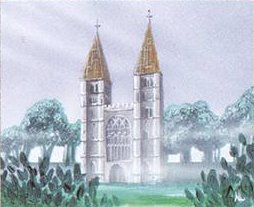
\includegraphics[width=\textwidth]{Tabernacle}
\pagenumbering{arabic}
\tableofcontents{}
%\chapter{Chapter 1: Overview and History}
%\chapter{Part 2: Core Cards - Pg 12\\}
%\chapter{Part 3: The Classic RG List - Pg 39\\}
%\chapter{Part 4: 2019 Metagame Changes Part One - Pg 53\\}
%\chapter{Part 4: New Lists Arising From 2019 Changes - "Dark Lands" - Pg 56\\}
%\chapter{Part 4: 2019 Metagame Changes Part Two - Pg 67\\}
%\chapter{Part 5: New Lists Arising From 2019 Changes - Pg 72\\}
%a) BUG List -  Pg 72\\
%b) RUG List - Pg\\
%\textbf{Part 6: New Lists Arising From 2020 Changes - Pg X\\}
%c) UG List - Pg\\
%\textbf{Appendix\\}
%A) Spice\\
%B) Probabilities and Loaming vs Drawing.
\chapter{History and Overview}
Lands is a unique toolbox prison-control based deck centered in green that seeks to eek out incremental value out of its, you guessed it, lands, and ultimately run down opponents on resources while presenting inevitability.\\ It employs powerful one mana tutors like \emph{Crop Rotation} and \emph{Gamble} to find the land necessary to answer any potential problem or the engine, \emph{Life from the Loam}, while seeking to abuse additional land drops/mana acceleration via \emph{Exploration}, \emph{Manabond} and \emph{Mox Diamond} to obtain an advantage over opponents. \\
In terms of its prison elements, while similar strategies (Red Prison, Eldrazi Stompy etc) mainly employ a \emph{lockpiece} (\textbf{Blood Moon, Chalice of the Void}) to disable large swathes of opposing decks, Lands instead opts for a similar strategy but employs different means and methods. Red Prison for example often sacrifices card quality (\textbf{Chrome Mox, Simian Spirit Guide}) to play a "bomb", while Lands uniquely cycles through its deck via Life from the Loam (akin to Ancestral Recall in the deck), its principal engine, and the various utility lands it pitches to the graveyard such as \textbf{Wasteland, The Tabernacle at the Pendrell Vale,} or \textbf{Rishadan Port}, which allow for a slow but inexorable stranglehold against many decks before closing the game out via one of several cards, \textbf{Dark Depths - Thespian's Stage}, lands that become creatures, aptly called \emph{Man-lands}, or the newly arrived \textbf{Field of the Dead}.\\
Its control element instead stems from its ability to gain card advantage via Life from the Loam, ignoring 1-1 trades and countermagic, coupled with gaining an advantage by making multiple land drops each turn while stalling opponents via cards like \textbf{Rishadan Port} or \textbf{Wasteland}. Given the "uncounterability" of making simple land drops and dredging Life from the Loam, effectively making countermagic a losing prospect, it quickly buries opponents in card advantage, while slowing down their ability to play Magic by attacking their mana.
\newpage
\paragraph{Origins and First Developments\\\\}
\begin{center}
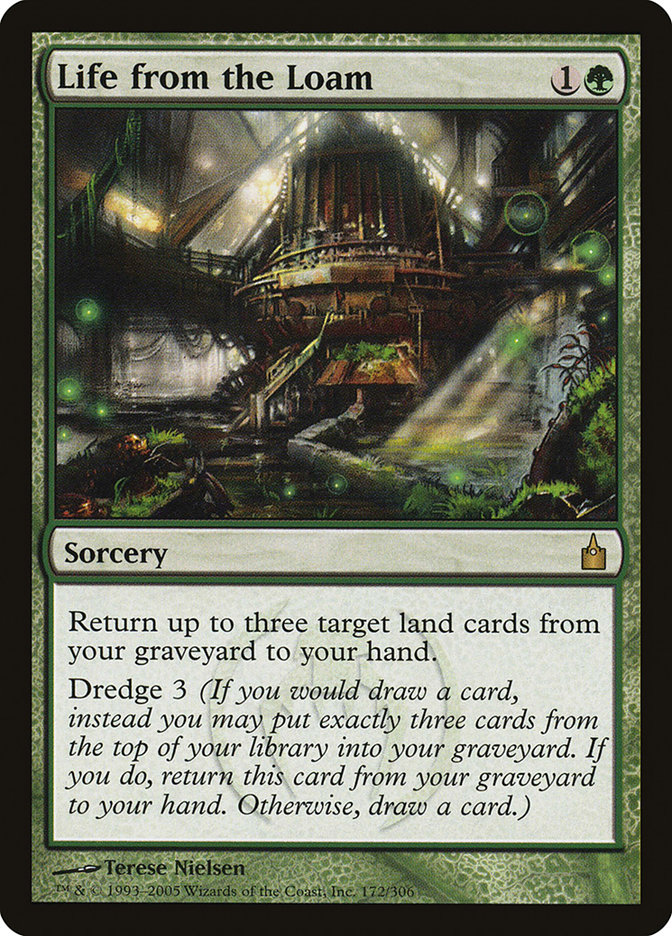
\includegraphics [width = 4cm, height = 6cm] {life-from-the-loam}\\
\end{center}
Lands has long been a staple of the legacy metagame/scene, tracing its roots back to the appearance of one of the most infamous mechanics ever, long been a point of contention: Dredge. \textbf{Life from the Loam}, appearing in the 36th expansion titled Ravnica: City of Guilds released on October 7th, 2005, birthed the Lands archetype as a whole, allowing for repeated usage and cycling of unique lands, (to name a few \textbf{Wasteland}, \textbf{The Tabernacle at Pendrell Vale}, \textbf{Rishadan Port}) and land drops to gain incremental advantage.\\\\
 In this period Lands was very much a control deck, using, among others, the aforementioned lands to gain an edge, while relying on artifacts such as Engineered Explosives as a general answer to troublesome permanents that could arise, recursion of artifacts via \textbf{Academy Ruins}, while cards like \textbf{Barbarian Ring}, \emph{Man-Lands} like \textbf{Mishra's Factory} or \textbf{Nantuko Monastery}, and even \textbf{Mindslaver} functioned as win conditions once a position of dominance had been established over the opponent.
\newpage
\begin{center}
\textbf{Old pre Depths Style List}
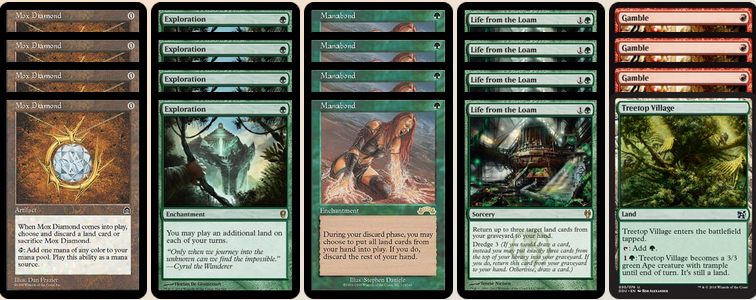
\includegraphics[width=\textwidth]{blast1}
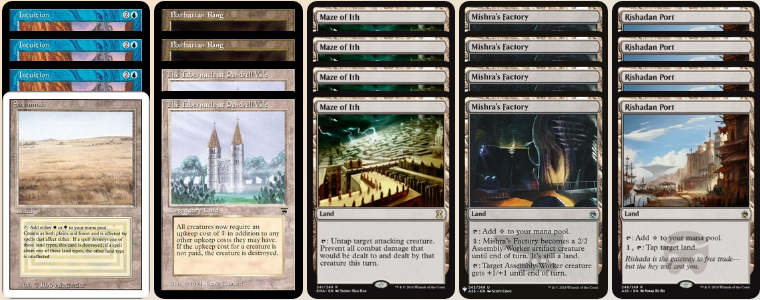
\includegraphics[width=\textwidth]{blast2}
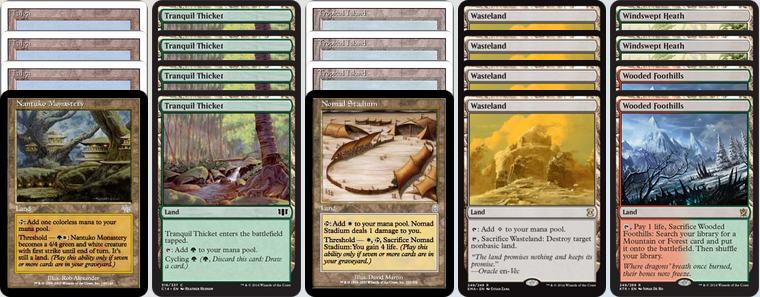
\includegraphics[width=\textwidth]{blast3}
\end{center}
However, the main pitfall of the deck was the length of time most games required, as a fast means of winning was simply non-existent. 
This would eventually change, thanks to a technicality.\\
\newpage
\paragraph{First Evolution: The transition to a more focused combo deck\\\\}
On July 19th 2013, the archetype would be forever changed, as an update to the game rules rules was enacted, in particular a revision of the so called "Legend Rule", which reads as follows:\\\\
\textbf {\emph{Rule 704.5j If a player controls two or more legendary permanents with the same name, that player chooses one of them,and the rest are put into their owners’ graveyards. This is called the “legend rule.”\\\\}}
This allowed, as part of a State Based Action, one to choose which legendary permanent would be kept in play should two appear on the battlefield at any given time. \\Thus, together with the printing of\textbf{Thespian's Stage} in the 2013 expansion titled "Gatecrash", it became possible to copy \textbf{Dark Depths}. This combo element, requiring only 2 mana along with Dark Depths and Thespian's Stage to be present on the battlefield, as then the controller of Thespian's Stage may copy Dark Depths, resulting in a Depths without any ice counters and thus triggering its "sacrifice" clause, resulting in the creation of the token.\\
Not to mention the inherent power of playing a potential 8 copies of any land, the printing of Thespian's Stage and the modification of the Legend rule previously mentioned gave a much needed burst of speed to the deck, permitting it to close out games far faster than before.\\\\
\textbf{The Combo:}\\
With 2 Mana and both lands on the battlefield, one may copy Dark Depths with Thespian's Stage to create the token.
\\\\
This works in the following way:\\
1) Designate Dark Depths as the target of the copy ability of Thespian's Stage.\\
2) Thespian's Stage copy ability resolves, and now two Dark Depths are present on the battlefield under our control, one with N > 0 ice counters and one with none.\\
3) As part of the "Legend Rule", we are required to choose which Dark Depths we want to keep, and naturally we choose the one with no counters on it.\\
4) Dark Depths' "sacrfice clause" triggers, and we sacrifice it to make a 20/20 indestructible Marit Lage Token.\\
This can be done as early as turn 1, with the following sample hand : \\Thespian's Stage, Dark Depths, Riftstone Portal, Mox Diamond, Mox Diamond, Exploration, any land.
The combo is often presented on turn 2 or later however, depending on the matchup.\\
Thus the archetype moved away from its older RUG version, relying on artifact recursion and man-lands to win, to a more combo focused one, eschewing some of the controlling elements to make the Depths-Stage interaction more consistent and easier to assemble.
\begin{center}
\textbf{Jody Keith's 1st Place List, SCG Atlanta 07/23/2017}\\ (Slight Variation)
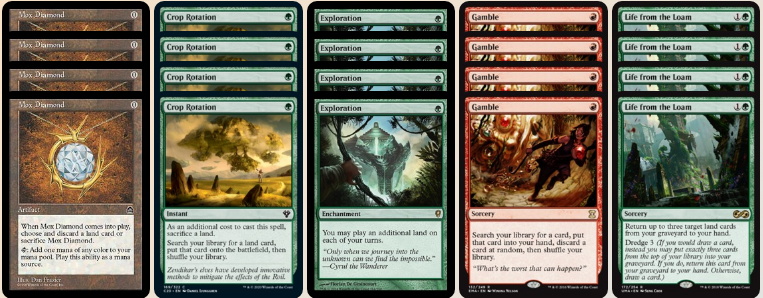
\includegraphics[width=\textwidth]{jodykeithlist1}
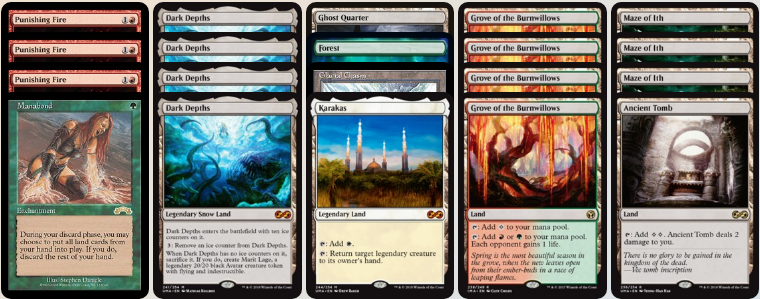
\includegraphics[width=\textwidth]{jodykeithlist2}
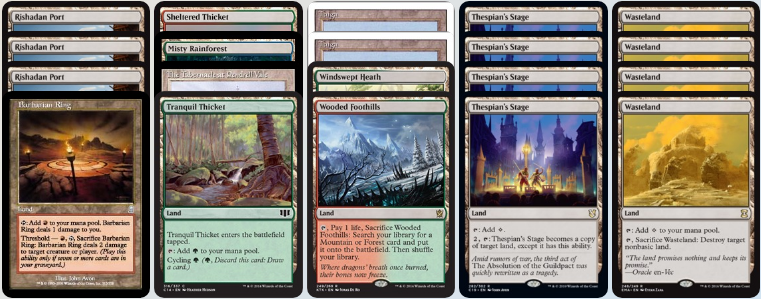
\includegraphics[width=\textwidth]{jodykeithlist3}
\newpage
\textbf{Sideboard}
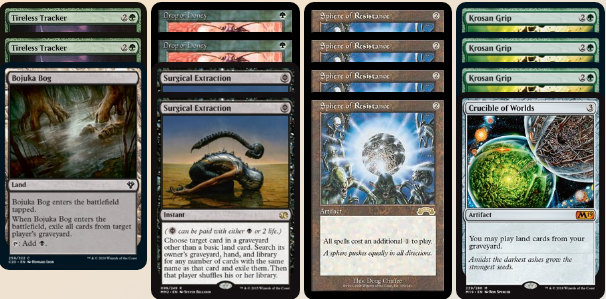
\includegraphics[width=\textwidth]{jodykeithlistsb}
\end{center}
\begin{comment}
Maindeck:\\
4 Crop Rotation\\
4 Exploration\\
4 Gamble\\
4 Life from the Loam\\
1 Manabond\\
4 Mox Diamond\\
3 Punishing Fire\\
1 Ancient Tomb\\
1 Barbarian Ring\\
4 Dark Depths\\
1 Forest\\
4 Ghost Quarter\\
1 Glacial Chasm\\
4 Grove of the Burnwillows\\
1 Karakas\\
3 Maze of Ith\\
1 Misty Rainforest\\
1 Sheltered Thicket\\
2 Taiga\\
1 The Tabernacle at Pendrell Vale\\
4 Thespian's Stage\\
1 Tranquil Thicket\\
4 Wasteland\\
1 Windswept Heath\\
1 Wooded Foothills\\\\
Sideboard\\
1 Bojuka Bog\\
1 Crucible of Worlds\\
2 Drop of Honey\\
3 Krosan Grip\\
4 Sphere of Resistance\\
2 Surgical Extraction\\
2 Tireless Tracker\\
\end{comment}
This list is what could be considered \emph{standard}, \emph{stock}. It is the tried and true formula, the most common \emph{form} of Lands known today. 
However, as time went on, Legacy and Magic as a whole underwent serious upheavals due to changes in design philosophy, and the tried and true core was shown to be lacklustre in certain areas, requiring supplemental cards to address such. 
\newpage
\paragraph{Legacy after 2015\\\\}
During the period between the beginning of 2016 and the Spring of 2017, Legacy enjoyed a stable, if arguably somewhat stagnant, metagame.\\ Lands was positioned as one of the top decks, given its ability to prey on control decks like  UW Miracles, generally accepted as one of the premier decks of the format during this time period, whose relatively useless creature removal in the form of Terminus and Swords to Plowshares coupled with the inefficiency of its countermagic in the face of the Loam engine would ensure that Lands enjoyed a privileged position in the matchup.\\Adding to this the power of Tabernacle and the ability to deal with fair creature decks, Lands' position as one of the better decks in the format was all but assured.\\ Many matchups presented little to no problems, outside of the matchups that are notoriously hard (fast combo mainly in the form of Reanimator and Sneak and Show/Omnitell).\\
\paragraph{2017 - 2019\\\\}
However, in April 2017 Miracles saw the banning of \textbf{Sensei's Divining Top}, due to time constraints during matches, a fulcrum of the deck in tandem with \textbf{Counterbalance} and the various "miracle" cards like \textbf{Terminus} and \textbf{Entreat the Angels}, resulting in a definite decrease in power level of the Miracles deck, and the rise of 3 and 4 colour decks (called "piles", as they played piles of good cards), powered by \textbf{Deathrite Shaman}.\\ This went on for a while, to the detriment of Lands, as the "one mana planeswalker" could exile both our engine \textbf{Life from the Loam} and the plethora of singleton Lands played as a toolbox. \\
This continued until \textbf{Deathrite Shaman} and \textbf{Gitaxian Probe} were found to be "too good" in Grixis (UBR) Delver, which had once again  as the former allowed for turn 2 \textbf{True Name Nemesis}, fixed mana and made splashes trivial thanks to the power of fetchlands, all the while presenting a clock, whereas the latter, being a free spell a vast majority of the time, made churning through one's deck far too easy.\\ Hence both cards left the format, and Lands was once again positioned to prey on the various decks in the format, now that its "Enemy N°1", had been eliminated from the format.\\\\
Then 2019 happened, and Legacy was changed forever.\\
\newpage
\paragraph{2019\\\\}
Undoubtedly, the year 2019 ushered in more changes for Legacy (and for other formats as well), and Magic as whole, than any other year hitherto. \\In the period between January 2019 and January 2020, many archetypes were revolutionized, many rendered obsolete.\\ New decks sprung up, and other decks fell into darkness. The format was irrevocably transformed, as set after set presented a flood of cards that completely reshaped the Legacy landscape, redefining Magic as a game and shaking it to its very foundations. (To highlight this shift in design, I have indicated which cards have been restricted or banned in one format or another)\\
In \textbf{\emph{chronological order}} the main sets that have come out since Jan 2019 are:\\\\
\textbf{-Ravnica Allegiance\\}
\textbf{-War of the Spark\\}
\textbf{-Modern Horizons\\}
\textbf{-Core 2020\\}
\textbf{-Throne of Eldraine\\}
\textbf{-Theros Beyond Death\\}
Among these, there are a slew of cards that have entered the meta and affected it to varying degrees, in chronological order (based on set) these are:\\\\
\textbf{Ravnica Allegiance\\}
-Cindervines\\
-Lavinia, Azorius Renegade\\\\
\textbf{War of the Spark\\}
-Dreadhorde Arcanist\\
-Narset, Parter of Veils \textbf{(Restricted in Vintage)}\\
-Teferi, Time Raveler\\
-Karn the Great Creator \textbf{(Restricted in Vintage)}\\
-Ashiok, Dream Render\\
-Tomik, Distinguished Advokist\\
-Ugin, the Ineffable\\
-Blast Zone\\
\textbf{\\Modern Horizons\\}
-Wrenn and Six \textbf{(Banned in Legacy)}\\
-Force of Negation\\
-Force of Vigor\\
-Arcum's Astrolabe\\
-Plague Engineer\\
-Collector Ouphe\\
-Ice-Fang Coatl\\
-Urza, Lord High Artificer\\
-Echo of Eons\\
-Hexdrinker\\
-Hogaak, Arisen Necropolis \textbf{(Banned in Modern)}\\
-Canopy Land Cycle (Sunbaked Canyon, Waterlogged Grove, Silent Clearing,\\ Nurturing Peatland, Fiery Islet)\\
-Prismatic Vista\\
-Dead of Winter\\\\
\textbf{Core 2020\\}
-Veil of Summer \textbf{(Banned in Standard and Pioneer)}\\
-Elvish Reclaimer\\
-Field of the Dead \textbf{(Banned in Standard and Pioneer)}\\
-Golos, Tireless Pilgrim\\
-Chandra, Awakened Inferno\\\\
\textbf{Throne of Eldraine\\}
-Oko, Thief of Crowns \textbf{(Banned in Standard, Pioneer and Modern)}\\
-Once Upon a Time \textbf{(Banned in Standard and Pioneer)}\\
-Wishclaw Talisman\\
-Brazen Borrower\\
-Mystic Sanctuary\\
-Emry, Lurker of the Loch\\\\
\textbf{Theros Beyond Death\\}
-Uro, Titan of Nature's Wrath\\
-Thassa's Oracle\\
-Underworld Breach \textbf{(Banned in Legacy)}\\
-Dryad of the Ilysian Grove\\
-Klothys, God of Destiny\\
While many of these cards stop certain archetypes in their tracks (Plague Engineer vs Tribal Decks, Teferi, Time Raveler in control matchups), of particular note for Lands are the following, which can be divided into \textbf\emph{{two}} groups:\\\\
\newpage
\textbf{Cards that improved Lands or Spawned new lists\\}
-Wrenn and Six\\
-Blast Zone\\
-Field of the Dead\\
-Force of Vigor\\
-Veil of Summer\\
-Elvish Reclaimer\\
-Uro, Titan of Nature's Wrath\\
-Oko, Thief of Crowns\\\\
\textbf{Cards that improved other decks' matchups against Lands\\}
-Wrenn and Six\\
-Force of Negation\\
-Arcum's Astrolabe\\
-Dreadhorde Arcanist\\
-Brazen Borrower\\
-Mystic Sanctuary\\
-Uro, Titan of Nature's Wrath\\
-Underworld Breach\\
Some of these, like \textbf{Uro, Titan of Nature's Wrath, Oko, Thief of Crowns, Field of the Dead, Force of Vigor,} and \textbf{Elvish Reclaimer}, have become stock in Lands lists, both in the main 60 and in the sideboard.\\\\Before continuing however, let's take a look at the core cards of the archetype.\\
\newpage
\chapter{Core Cards}
Lands, as its name would suggest, plays a very light, but exceptionally powerful, suite of spells. Spells it is aiming to resolve on the very first turns of the game, and then never worry about again. Outside naturally, of \textbf{Life from the Loam}.\\\\
\textbf{Life from the Loam\\}
\begin{center}
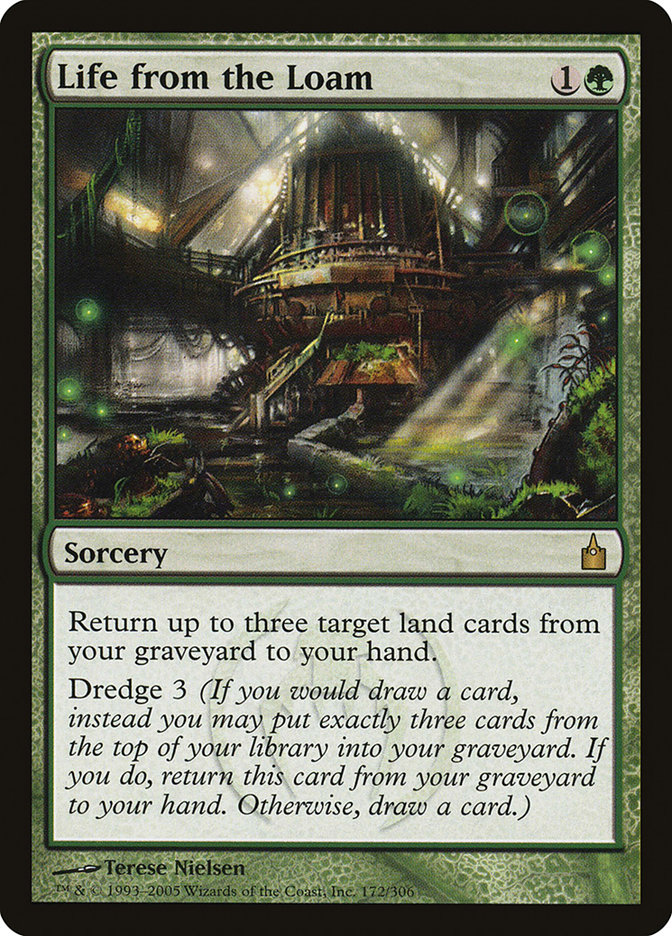
\includegraphics [width = 4cm, height = 6cm] {life-from-the-loam}\\
\end{center}
This is our bread and butter. This is what enables the deck to exist, and, in a deck full of lands, is often touted as the legacy legal "draw 3 cards" in this deck.\\It not only returns lands to hand to be used again, but enables digging for those lands as well, via the dredge mechanic.\\In conjunction with \emph{Wasteland}, it is a powerful tool for slowing our opponents down and wearing down their resources.\\ In conjunction with \emph{Thespian's Stage} and \emph{Dark Depths}, it allows us to represent a 20/20 monster ideally every turn.\\With silver bullet lands like \emph{Karakas}, \emph{Bojuka Bog}, \emph{The Tabernacle at Pendrell Vale} each whose value waxes and wanes according to the matchup, we can easily find and contrast our opponents gameplan.
It should go without saying, but never play less than 4 copies.\\
\textbf{Verdict: Play 4\\}\\
\textbf{Exploration\\}
\begin{center}
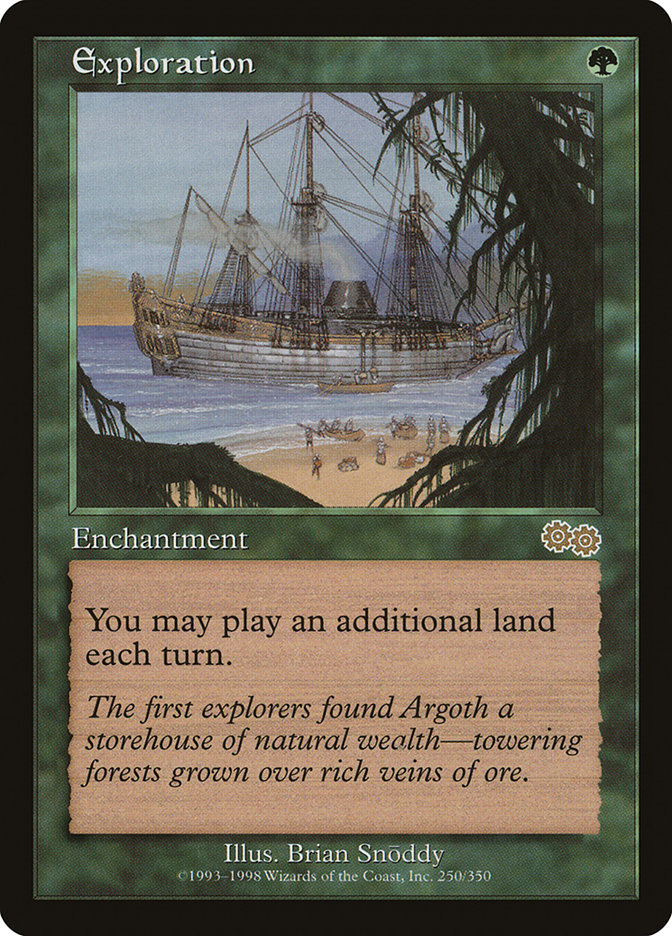
\includegraphics [width = 4cm, height = 6cm] {exploration}\\
\end{center}
While Loam is the deck's bread and butter, this card pushes the Loam engine over the edge. Allowing us to make multiple land drops per turn, it allows us to Wasteland/Port our opponent while putting us ahead on mana, permits us to assemble to combo every turn in the mid to late game, and is generally necessary to leverage Loam most effectively.\\Playing 4 copies ensures the probability of having it in one's opener, but generally copies 2-4 are redundant and often unneeded. You want to play no less than 4 copies.\footnote{\emph{Note}: There has been some back and forth on the number of copies to be played, but it is mainly a personal preference. The generally accepted standard is 4 copies,  however I know of some very successful Japanese players who prefer a 3-1 split between \textbf{Exploration} and \textbf{Manabond} (Hori Masataka, to name one such player), so your mileage may vary. It is mainly up to personal taste, but I wholeheartedly encourage playing no less than four.}\\
\textbf{Verdict: Play 4}
\newpage
\textbf{Crop Rotation}\\
\begin{center}
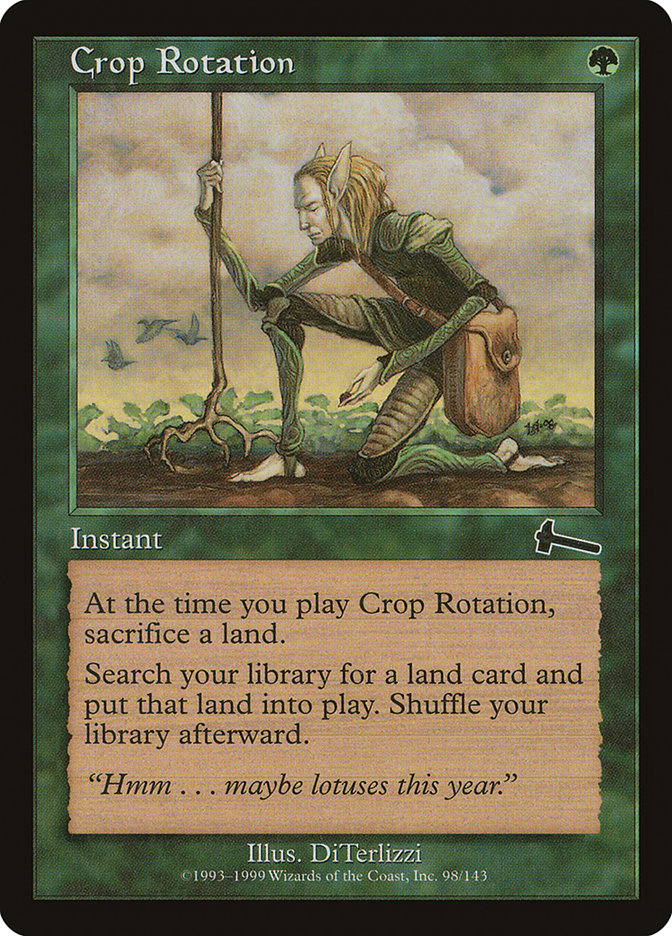
\includegraphics [width = 4cm, height = 6cm] {crop-rotation}\\
\end{center}
Often accurately called the \emph{"one mana land tinker"}, this card allows us to singlehandedly tutor a land from our deck, at instant speed, to answer any problem, for the low cost of one green mana and sacrifice of a land, which Loam naturally mitigates.\\This card allows for end of turn 20/20s, is a maindeck answer to a \textbf{Reanimate} on the stack thanks to \textbf{Bojuka Bog}, and is in general, a very powerful card.While being arguably one of the best cards in the deck however, given that sacrifice of a land is part of its castings costs, it loses equity in the face of counterspells, something to be considered while sideboarding. Playing 4 copies is a must, if one is playing \textbf{Dark Depths} and \textbf{Thespian's Stage}\\
\textbf{Verdict: Play 4\\\\}
\textbf{Mox Diamond\\}
\begin{center}
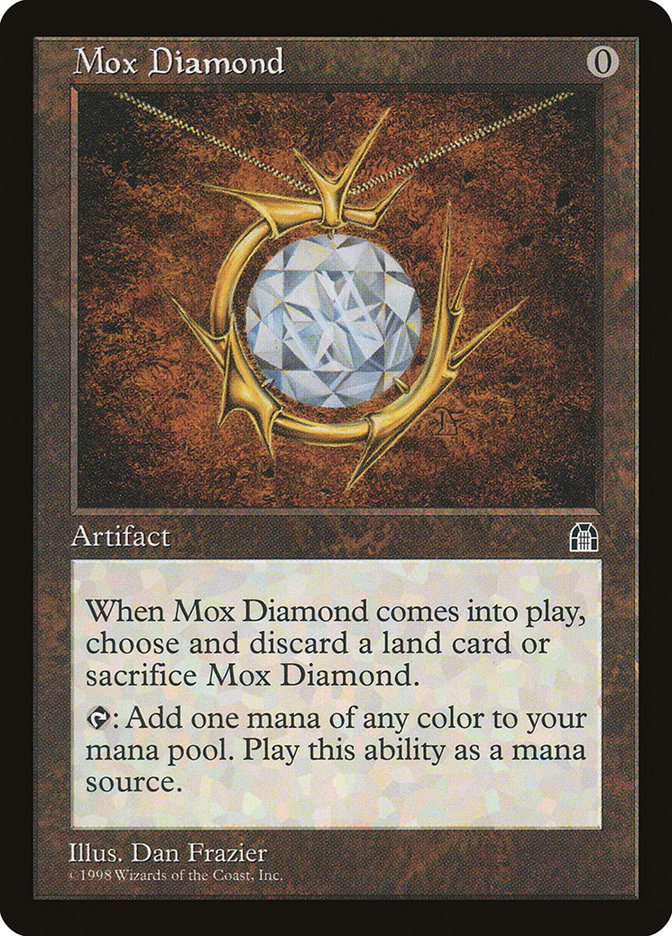
\includegraphics [width = 4cm, height = 6cm] {mox-diamond}\\
\end{center}
A necessary 4 of, it is one of the best cards in the deck in opening hands, allowing us to have 2 mana on turn 1 without any significant drawback thanks to Loam.\\ In many cases, playing a turn 1 Mox Diamond and loaming back the discarded land sets up our engine nicely while fixing our mana and putting us ahead of our opponents. In the lategame however, it can be a terrible draw. Still, 4 of is essential to ensure we have acceleration in our opening hand.\\
\textbf{Verdict: Play 4}\\\\
\textbf{Total: 16}\\\\\\\\
These are all the spells necessary to make the deck tick. Playing 16 spells gives us plenty of room to play all the \textbf{LANDS} we could ever want!\\
Note: Generally, a land count of 34-36 is the accepted standard. The 8-10 slots that remain give rise to the various flavours/colour combinations of Lands, which we will look at further down.\\
First however let us take a look at the lands suite typically played, and relegate them to 4 principal groups; \textbf{"Coloured Mana"}, \textbf{"Control/Mana Denial"}, \textbf{"Win Conditions"}, and \textbf{"Silver Bullets"}, as per their function.\\\\
\textbf{Group 1: Coloured Mana}\\
These lands let us cast our spells, and in some cases, serve as recursion.
The typical modern Lands manabase consists of:\\
6 untapped green mana sources/duals (in classic RG builds generally this is a \\2 Taiga - 3/4 Grove of the Burnwillows split)\\
1 Forest\\
3-5 Green Fetches (Verdant Catacombs, Misty Rainforest, Windswept Heath, Wooded Foothills).\footnote{Playing fetches that do not get green mana/basic forest are not worthy of consideration, as it is essential to have access to green mana for Life from the Loam. The basic forest allows us to play around Blood Moon and Back to Basics, making it essential in the deck, as well as giving us the ability to play Life from the Loam without worrying about opposing Wastelands.\\}
\\\\\textbf{Total: 10-12}\\\\
\textbf{Group 2: Control and Mana Denial}\\
The legacy format has a plethora of lands at the archetype's disposal by means of which it asserts its control in a matchup. This entails attacking decks upon 2 fronts, \emph{Mana Denial} and \emph{Creature Management}.
Our Mana Denial comes mainly from the legacy pillar \textbf{Wasteland}.
\begin{center}
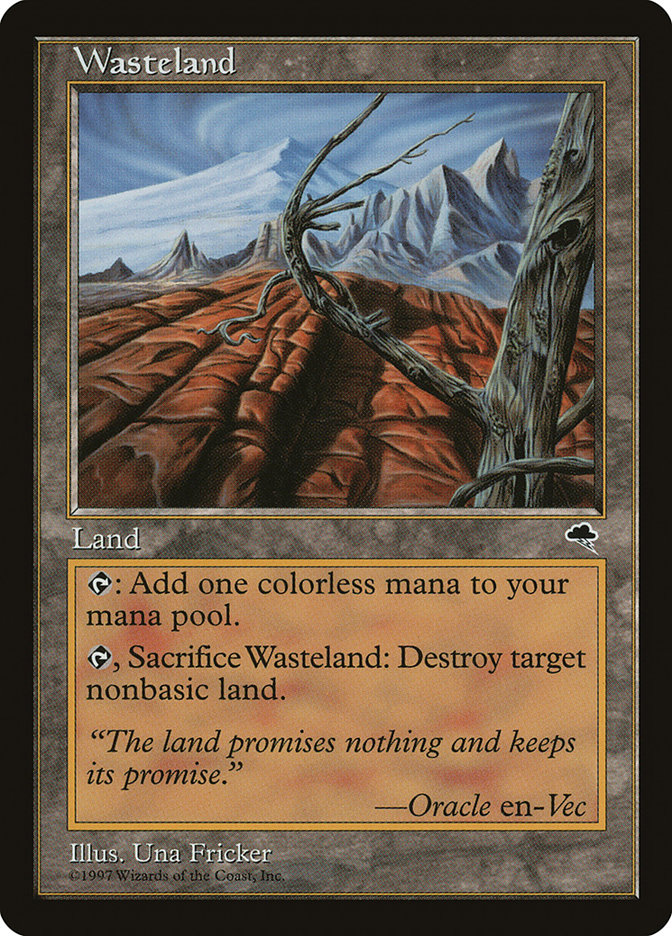
\includegraphics [width = 4cm, height = 6cm] {wasteland}
\end{center}
This card, already used to great success in several decks such as Delver and Death and Taxes where it represents a tempo play capable of putting an opponent off a colour and weakening their mana, and enables punishment of greedy manabases full of non basic lands, is taken to an extreme in Lands.\\In fact, differently from the previously mentioned decks which seek to use it as a tempo play, together with \textbf{Life from the Loam} it becomes a virtual win condition, as it impedes our opponent from playing Magic by cutting them off of the most fundamental of resources and often results in concessions.\\Never play less than 4.\\
\textbf{Verdict: Play 4\\\\}
Accompanying \textbf{Wasteland} is \textbf{Rishadan Port} for basic land hate, and is excellent for taxing our opponents mana in addition to cutting them off colours. Works wonders on creature decks with \textbf{The Tabernacle at Pendrell Vale}. Anywhere between 3-4 copies is where you want to be, as it is a boon in the faster combo matchups, allowing us to slow opposing decks down in order to get to the midgame and assert our various locks.
\footnote{Two things are of particular relevance, as follows:\\
1) Always activate Rishadan Port on your opponents lands \emph{after} your opponent has paid for Tabernacle triggers, not before. They pass priority in their upkeep after the Tabernacle triggers resolve, giving you a window to tax their mana further.\\
2) Rishadan Port can also be used proactively, if one has the means of assembling the combo on the end of an opponent's turn. Tapping down white sources is a great way to shut off potential Swords to Plowshares on our Marit Lage token, or turning off cards like Assassin's Trophy on our combo pieces.\\}\\\textbf{Verdict: Play 3-4}\\\\
\begin{center}
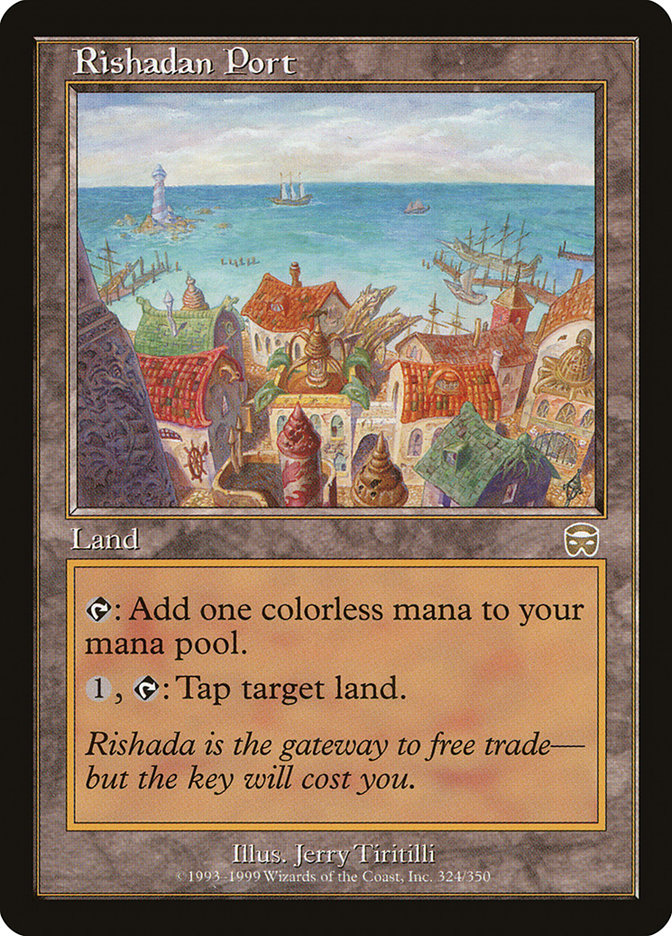
\includegraphics [width = 4cm, height = 6cm] {rishadan-port}
\end{center}
As an additional tool in our mana denial suite we have \textbf{Ghost Quarter}.
\begin{center}
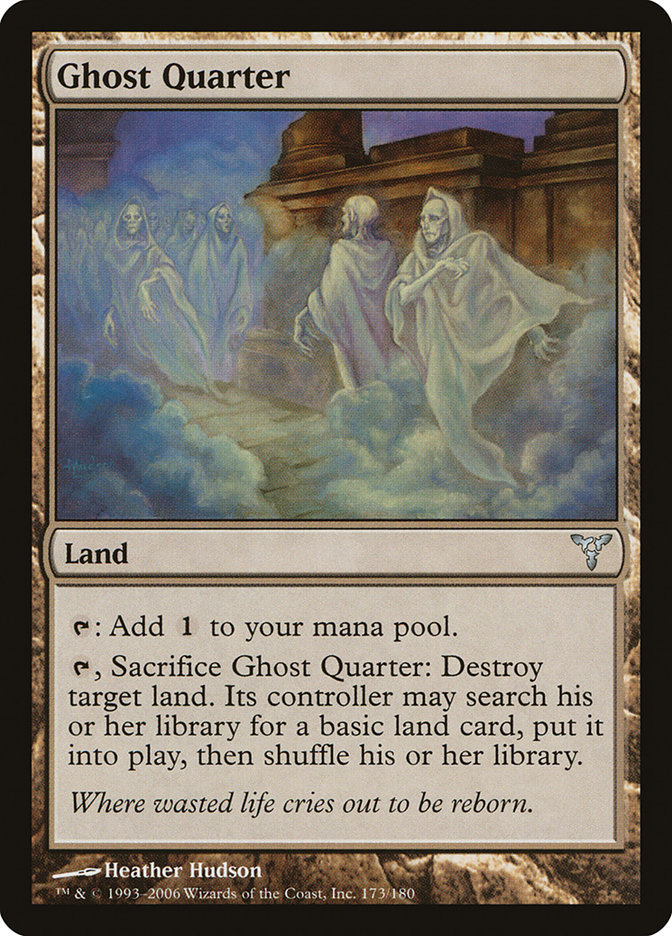
\includegraphics [width = 4cm, height = 6cm] {ghost-quarter}
\end{center}Effectively Wasteland number 5 in a non-zero number of matchups, it is preferable to have an additional way of destroying opposing lands in the face of cards like \textbf{Sorcerous Spyglass}, \textbf{Pithing Needle} and \textbf{Surgical Extraction} targeting Wasteland, allowing us to continue our mana denial plan even through these hindrances. At least 1 is the suggested amount, as it still gives our opponents basics.\footnote{1) Being a control deck at heart, piloting Lands correctly and optimally requires a certain metagame knowledge as well as a knowledge of opposing decklists. One key example of this is knowing how many basics on average any deck plays.\\Familiarizing oneself with such gives you an edge over your opponents, as you know how many Ghost Quarter activations are required before it becomes Strip Mine.  A good example of this is against Ad Nauseam Tendrils, which generally plays 2-3 basics, where cutting them off, say black mana, can mean the difference between a win and a loss.
2) Don't forget, you can use it to fix your own mana as necessary, thanks to the basic forest we play.}
\\\textbf{Verdict: Play 1\\\\}
\textbf{The Tabernacle at the Pendrell Vale}
\begin{center}
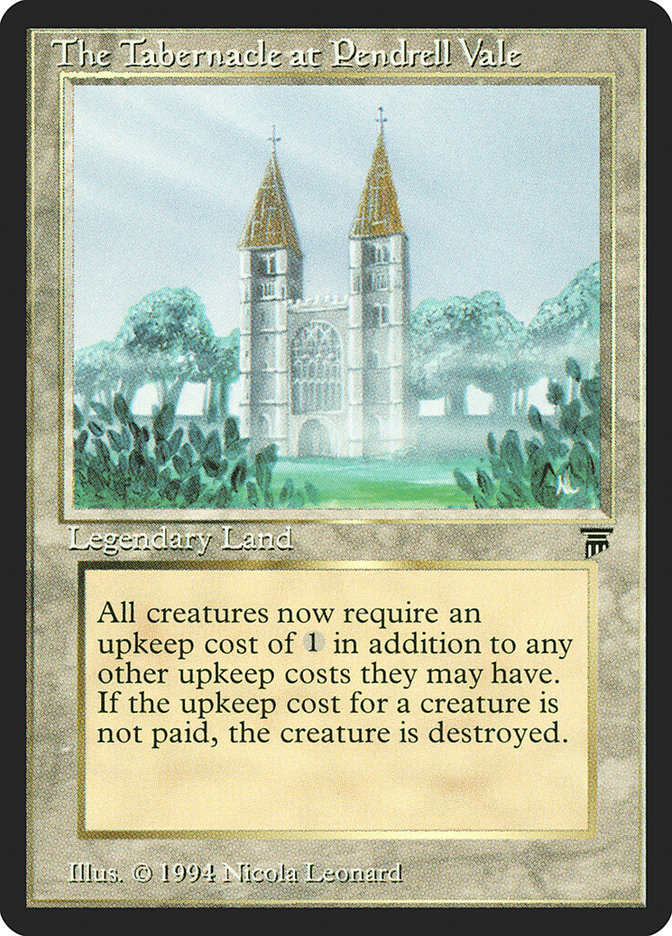
\includegraphics [width = 4cm, height = 6cm] {tabby}
\end{center}This is the crown jewel of our mana denial suite, and the best land in our deck. It singlehandedly turns entire matchups and boardstates in our favour, allowing us to beat otherwise unbeatable decks, such as Goblins, Elves, and turn 1 \textbf{Empty the Warrens}, just to name a couple.\\The land also severely hampers creature focused decks such as Death and Taxes and Maverick, while weakening go wide strategies presented by \textbf{Young Pyromancer} and \textbf{Monastery Mentor}.\\
\emph{Full Disclaimer}: \textbf{Yes}, the card is necesssary to play Lands.\\The deck loses a significant amount of its power without it and is mostly unplayable otherwise. Many unwinnable situations become trivial with this land on the battlefield. In the past 1-2 were played, between the main 60 and the side 15. Nowadays only 1 is necessary, but at least 1 is required.\footnote{1) Because of layers, \textbf{Oko, Thief of Crowns} +1 ability *removes* the Tabernacle effect creatures gain as they enter the battlefield. This is because Oko's +1 ability occurs in layer 4, , while Tabernacle's ability is applied in layer 6. This can be easily circumvented by replaying Tabernacle, if necessary.\\
2) Tabernacle's effect is worded such that the ability is given to each creature, hence the creature's controller owns it. They are therefore required to remember it in their upkeep.\\
3) Tabernacle's effect \textbf{destroys} a creature. Therefore, indestructible creatures are immune to its effect. This naturally applies to Marit Lage as well.}\\
\textbf{Verdict: Play 1}\\
\newpage
\textbf{Control}\\
Control instead principally comes in the form of 2 cards, \textbf{Maze of Ith} and \textbf{Glacial Chasm}.
Where Tabernacle punishes go wide strategies, Maze of Ith punishes go tall strategies, keeping us from taking lots of damage off one large creature, main ones being Tarmogoyf and Gurmag Angler. We generally want 1 in a list, but many play 2+, as it has synergy with \textbf{Oko, Thief of Crowns}.
\\\textbf{\emph{Verdict: Play 1\\\\}}
\begin{center}
\textbf{Glacial Chasm and Maze of Ith\\}
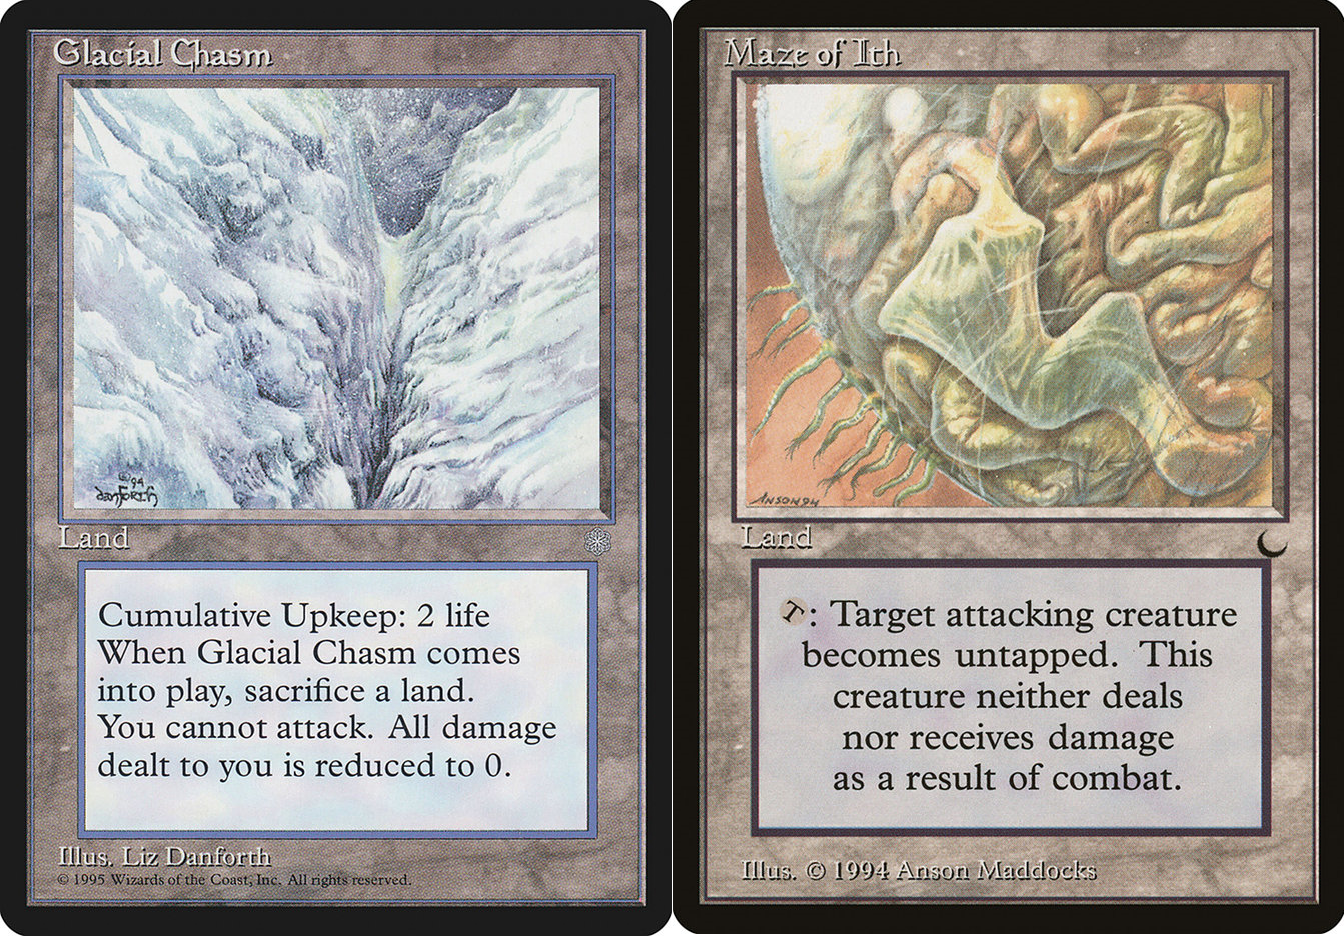
\includegraphics [width = 8cm, height = 6cm] {chasm-maze}
\end{center}
In the same vein, \textbf{Glacial Chasm}, with its unique and powerful ability, used to be a staple in the deck as a means of preventing damage. Given once again however the increase in speed and the "Wrenn and Six" era in particular,\\ while still a valuable tool every Lands player should have in their arsenal,\\"Wastelanding" oneself (in terms of the sacrifice clause on Glacial Chasm) to stave off a loss has become less than ideal, as other, arguably more powerful cards that both fill the same role and yet have other uses.\\The main reason for it falling out of favour is the logic that it "keeps you from losing" rather than "helps you win".\\ 0-1 copies are advised, especially if you find yourself playing against a lot of Burn or Tribal decks like Elves or Merfolk.\\
\\\textbf{\emph{Verdict: Play 0-1\\\\}}
\textbf{Total: 10-13}
\newpage
\textbf{Group 3: Win Conditions}\\
As mentioned before, Lands used to win via "Man-Lands" like \textbf{Nantuko Monastery/Creeping Tar-Pit} or \textbf{Mishra's Factory}  as well as \textbf{Barbarian Ring} to burn opponents out. This however made for terrible matchups against faster decks, not to mention causing many games to go to time. \\This all changed, as mentioned before, with the change in the legend rule, and gave us new win conditions.\\\\
\textbf{Thespian's Stage\\}
\begin{center}
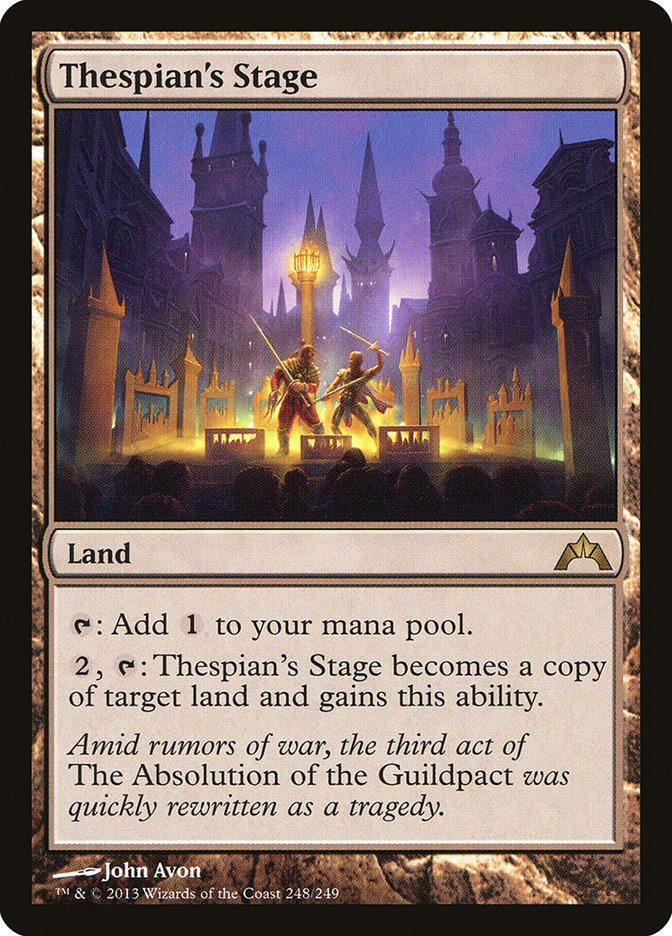
\includegraphics [width = 4cm, height = 6cm] {thespian-stage}
\end{center}
\emph{Thespian's Stage} is another one of the best cards in our deck. For a meagre 2 mana, it allows us to play extra copies of any land in our deck, giving us a win condition when paired with Dark Depths, extra utility with Wasteland and Rishadan Port, and general shenanigans an experienced player can leverage. We play no less than 4 copies.\footnote{1) Thespian's Stage, as mentioned previously, has a number of uses a skilled player can take advantage of. The first one being that it can copy \emph{any} land, not just lands under your control. This is essential, for example, in the mirror or against Depths decks, since you may simply copy their Depths, something a novice player may be unaware of, causing blowouts. This is true for \textbf{Karakas} and other utility lands as well, however, beware of your own Dark Depths and opponent's Stages!\\
2) Thespian's Stage can obviously be used to fix one's mana in the face of Wasteland. Copied basic lands retain Stage's ability as well, and gain the "basic" supertype, preventing opposing Wastelands until you are ready to combo.\\
3) Thespian's Stage has a unique interaction with Glacial Chasm. Since Chasm's cumulative upkeep is a triggered ability and uses the stack, you may respond to the trigger by copying Chasm, and then keeping the Thespian's Stage - Chasm instead of the original Chasm, resulting in no life loss and preventing instant speed loss via direct damage spells. The same can be done when playing Chasm, as its ETB ability can be answered by copying it, and then Chasm may be sacrificed to itself, allowing you to retain a copy of it.\\
4) If an opponent plays a Pithing Needle effect with the intention of naming Thespian's Stage, you may simply choose to copy another land, as the copied land retains Thespian's Stage's ability.}
\textbf{Verdict: Play 4\\\\}
\textbf{Dark Depths}
\begin{center}
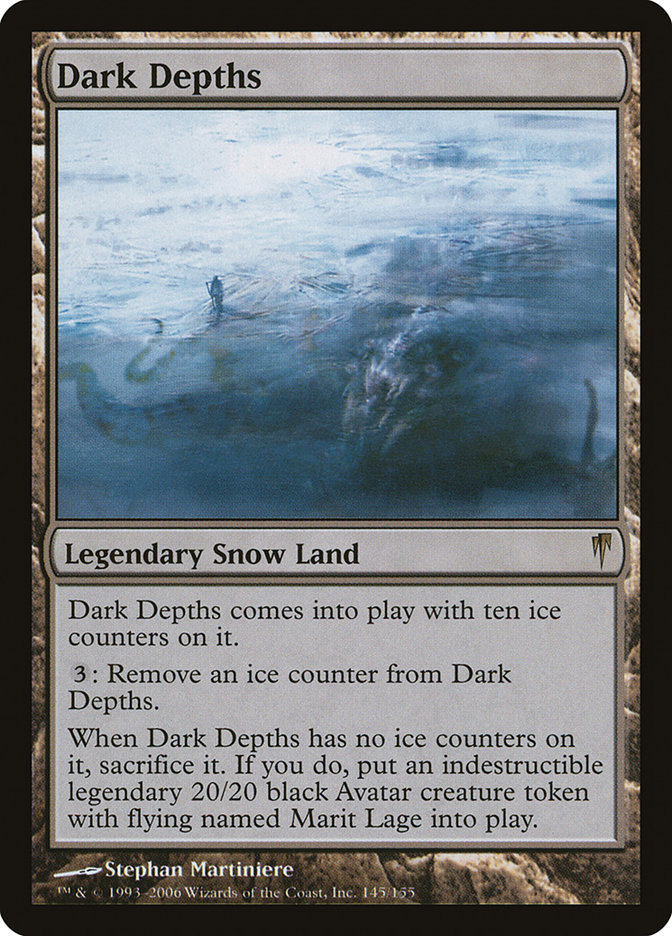
\includegraphics [width = 4cm, height = 6cm] {dark-depths}
\end{center}
\textbf{Dark Depths} is the second and essential half to our 2 card combo as well as main win condition, as it allows us, via copying with Stage, to produce at instant speed a Lovecraftian 20/20 indestructible tentacle monster.\\However, the fact that it does not tap for mana, makes it somewhat of a liability, and in certain slower matchups its position as premier win condition has been usurped by Field of the Dead.\\ However, in our harder matchups, mainly Reanimator, Sneak and Show and Storm variants, it is still the kill of choice given its speed. Play at least 3, 4 in a combo heavy meta.\footnote{As of 29-09-2017, there was a change in the interaction between Blood Moon and Dark Depths. Previously, a Dark Depths played after a Blood Moon would retain its counters; this is no longer true according to the following rules change:
"If a nonbasic land has an ability that causes it to enter the battlefield tapped, it will lose that ability before it applies. The same is also true of any other abilities that modify how a land enters the battlefield or apply “as” a land enters the battlefield, such as the first ability of Cavern of Souls. This is a change from previous rulings."
This means that if the Blood Moon is removed, the Depths' "sacrifice clause" triggers and a Marit Lage can consequently be created.}
\\\textbf{Verdict: Play 3-4\\}
\newpage
\textbf{Field of the Dead}\\
\begin{center}
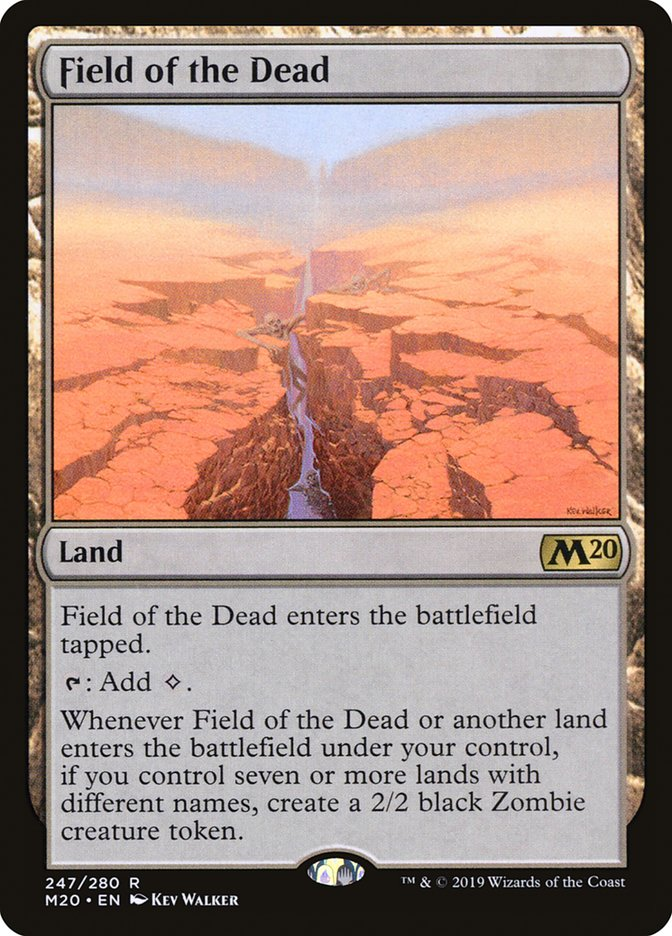
\includegraphics [width = 4cm, height = 6cm] {field-of-the-dead}
\end{center}
\textbf{Field of the Dead} is one of the newest, and yet most powerful cards the archetype has received since its inception. Its ability to produce an inexorable influx of Zombies makes it impossible for some decks to beat, especially in the slower, more grindy matchups.\\ The card is very good against control (UWx Miracles/Astrolabe) and grindy (3 and 4c UBx) decks, as it completely nullifies the one for one trades these decks typically are looking to make, while pressuring opponent's life totals and planeswalkers.\\ Somewhat difficult to turn on in the faster matchups, and weak against \textbf{Wasteland} heavy decks, the card is still phenomenal in certain matchups, outclassing even the Depths-Stage Combo.\\
At least 1 copy should be in every 60, and some even play 2.
\\\textbf{Verdict: Play 1-2\\\\}
\textbf{Total 7-10}\\

\paragraph{Group 3: Silver Bullets\\}
A number of lands are invaluable in certain matchups and should be played as at least 1 ofs. These are, in no particular order, the following:\\
\newpage
\textbf{Blast Zone}\footnote{Be aware of the fact that Blast Zone can also take care of 0 converted mana cost permanents, such as creature tokens. Simply copy it with \textbf{Thespian's Stage}, and then activate its ability, as the copy will not have a charge counter on it.}
\begin{center}
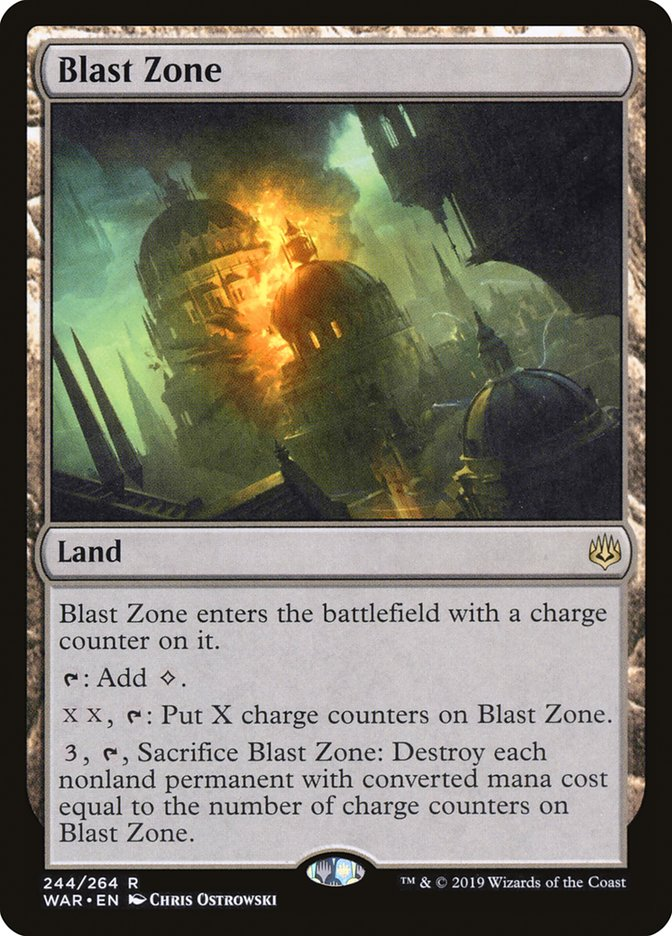
\includegraphics [width = 4cm, height = 6cm] {blast-zone}
\end{center}
Engineered Explosives on a land? What's not to like? This card is nuts, it lets us easily clear the board from troublesome permanents/threats, and can be recurred via Life from the Loam. A No Brainer.\\\textbf{Verdict: Play at least 1}
\textbf{\\Karakas}
\begin{center}
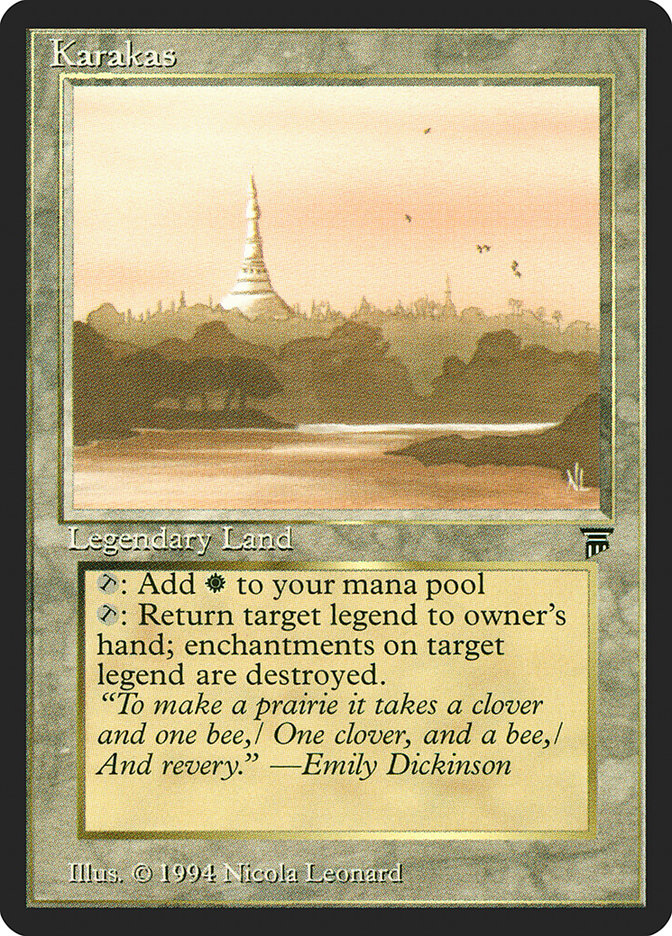
\includegraphics [width = 4cm, height = 6cm] {karakas}
\end{center} Returns legendary creatures to hand. Great for opposing Marit Lages or troublesome legendary creatures like \textbf{Questing Beast} and \textbf{Tomik, Distinguished Advokist}, or even a reanimated \textbf{Griselbrand} or an \textbf{Emrakul, the Aeons Torn} put in off \textbf{Show and Tell}. Rather self explanatory, given the abundance of legendary creatures present in legacy. The fact that it taps for white mana is also relevant in some builds of Lands.
\textbf{Verdict: Play 1}\\
\newpage
\textbf{Horizon Canopy/Waterlogged Grove/Nurturing Peatland}:\\
\begin{figure}
  \begin{subfigure}[b]{.325\textwidth}
\begin{center}
    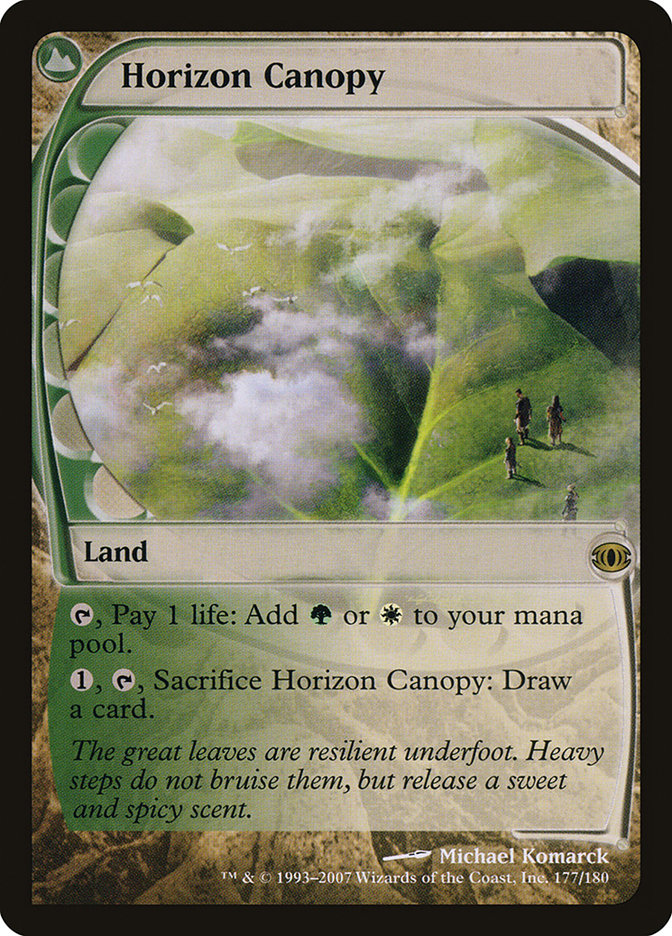
\includegraphics [width = 4cm, height = 6cm] {horizon-canopy}
    \caption{Horizon Canopy}
    \label{fig:1}
\end{center}
  \end{subfigure}
  %
  \begin{subfigure}[b]{.325\textwidth}
\begin{center}
    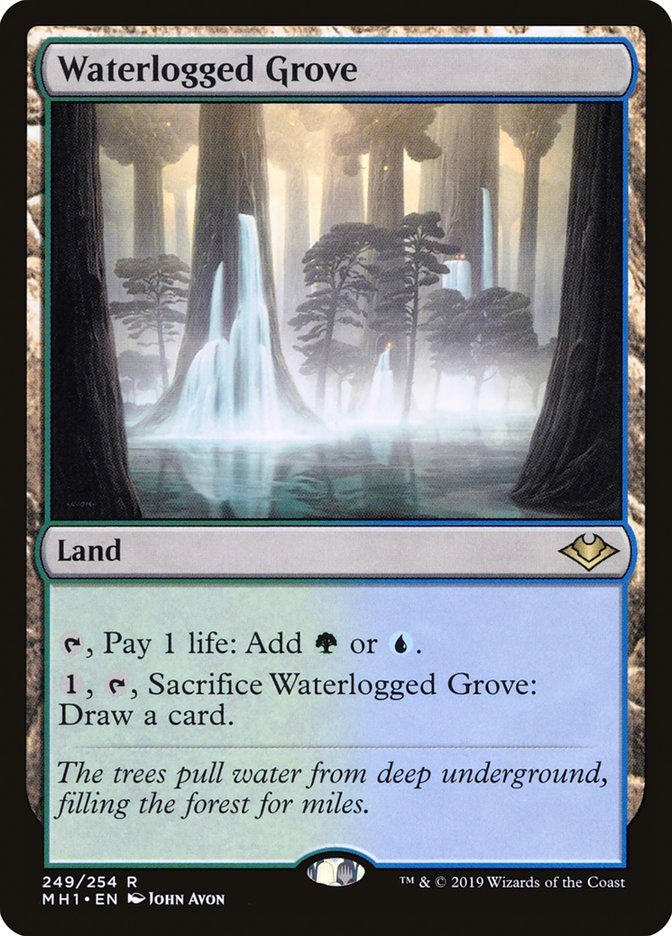
\includegraphics [width = 4cm, height = 6cm] {waterlogged-grove}
    \caption{Waterlogged Grove}
    \label{fig:2}
\end{center}
  \end{subfigure}
%
  \begin{subfigure}[b]{.325\textwidth}
\begin{center}
    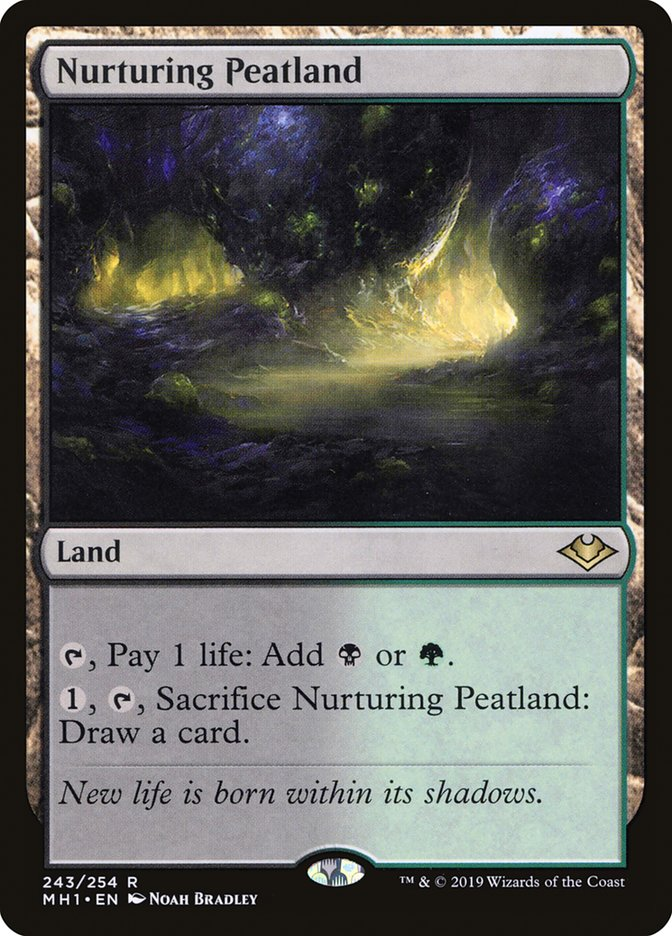
\includegraphics [width = 4cm, height = 6cm] {nurturing-peatland}
    \caption{Nurturing Peatland}
    \label{fig:3}
\end{center}
  \end{subfigure}
\end{figure}
\\Known also as "Canopy Lands", this card is one of 3 draw "spells". It allows us to accrue card advantage independently of Loam, together with its cousin, \textbf{Tranquil Thicket}, while tapping for coloured mana and entering the battlefield untapped.\\Modern Horizons brought us both Waterlogged Grove and Nurturing Peatland, opening up the possibility of playing better on colour lands. This life loss however can add up, so one copy is sufficient.\footnote{1) While repeatedly offering a means of card advantage in tandem with Loam, it also, when coupled with Crop Rotation, allows us to save a Loam at instant speed from Surgical Extraction, as long as we have 2 mana (1 Green, one generic) open.\\This works in the following way:\\
		a) Opponent targets Loam as part of Surgical Extraction's casting\\
		b) We Crop Rotate in response for our canopy land.\\
		c) We activate the draw part of the canopy land, sacrificing it to take a draw\\
		d) As part of the replacement effect Dredge offers, we choose to dredge the targeted Loam instead of drawing, thus saving Loam from Surgical Extraction and causing it to fizzle, effectively countering it.}\\
\textbf{Verdict: Play 1}\\\\
\textbf{Tranquil Thicket} is the second of our draw "spells", while also tapping for green. It however, has the added advantage of drawing a card immediately (and can save Life from the Loam from Surgical Extraction similarly to a canopy land, by activating Thicket in response) rather than using up a land drop.\\ It has the downside of only tapping for G and entering the battlefield tapped. Still, a worthy inclusion that should be in the main 60.\\
\textbf{Verdict: Play 1}\\
\begin{center}
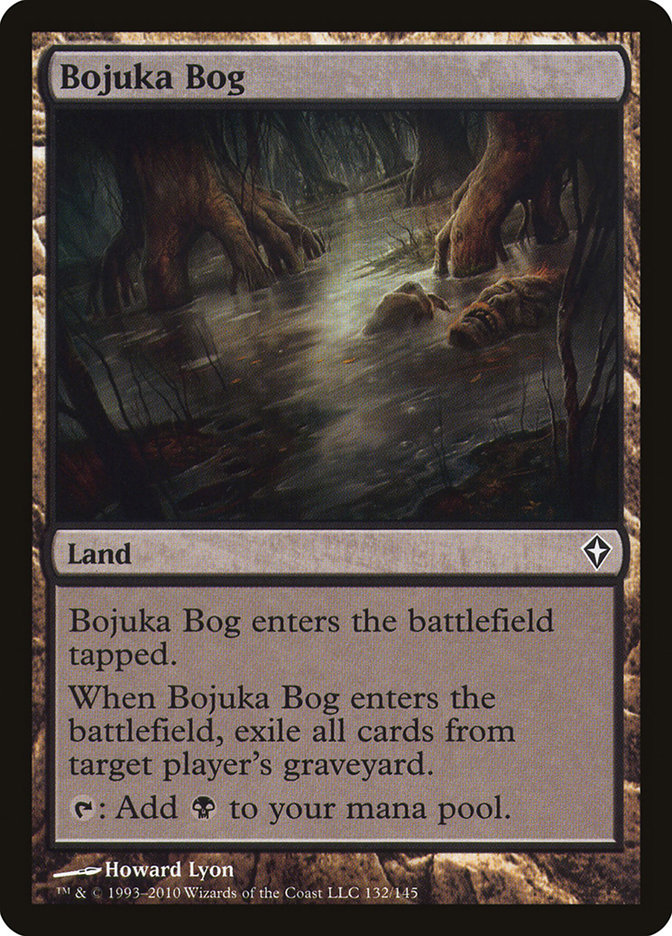
\includegraphics [width = 4cm, height = 6cm] {bojuka-bog}
\end{center}
\textbf{Bojuka Bog} allows us to have game before sideboarding against Reanimator and the various Hogaak/Dredge/Graveyard based decks, as its ability occurs upon ETB, which can be potent when accompanied by \textbf{Crop Rotation}.\\It is also great against generic cards that seek to gain advantage by means of the graveyard, for example \textbf{Dreadhorde Arcanist}, \textbf{Gurmag Angler}, \textbf{Tarmogoyf},\textbf{Mystic Sanctuary}, and \textbf{Uro, Titan of Nature's Wrath} to name a few.\\Its ability to tap for black mana is relevant in some builds of Lands.\\
\textbf{Verdict: Play 1}\\\\
\begin{center}
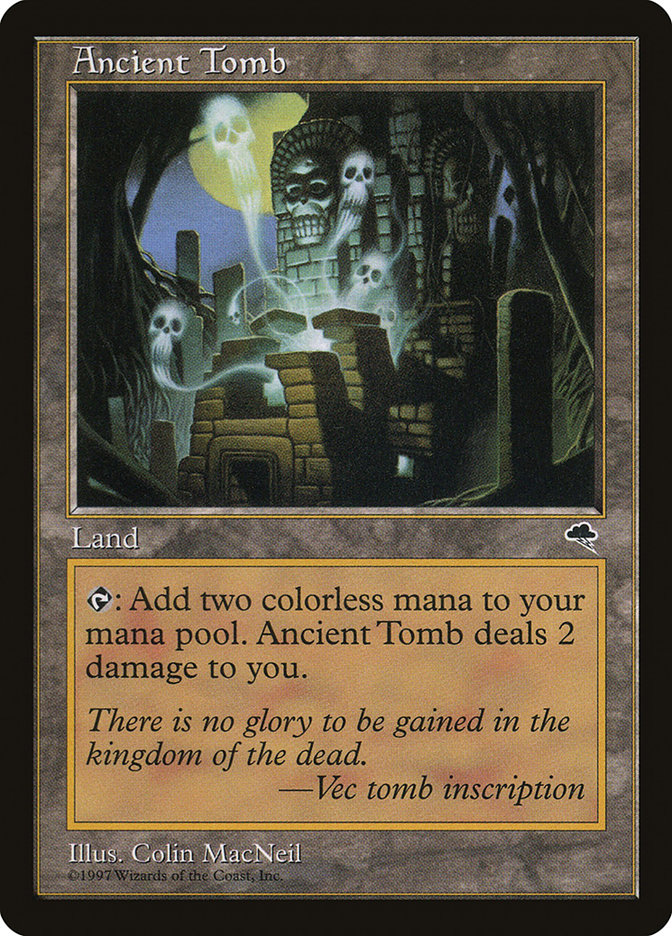
\includegraphics [width = 4cm, height = 6cm] {ancient-tomb}
\end{center}
\textbf{Ancient Tomb} is not necessarily a mainstay of most lists, and in some cases is a relic of the past, as it does not tap for coloured mana, and damages ourselves. However, I believe the ability to play turn artifacts from the sideboard such as \textbf{Sphere of Resistance}, \textbf{Thorn of Amethyst} or \textbf{Chalice of the Void} on turn 1 make it a excellent main deck inclusion.\\ It also makes copy other lands easier, and in general gives a much needed burst of speed to the deck in some cases, outweighing the life loss. Playing either in the maindeck or in the sideboard is highly recommended.\footnote{1) Playing Ancient Tomb maindeck, in addtion to making your Stages easier to activate, also allows you to play turn 1 Spheres or other 2 mana artifacts with higher probability than without, simply because the cards required to assemble a lockpiece and the necessary mana to cast it are less in a deck with Ancient Tomb than a deck without (more on probabilities in the appendix).}\\
\textbf{Verdict: Play 0-1}\\\\
\textbf{Sheltered Thicket}\\
\begin{center}
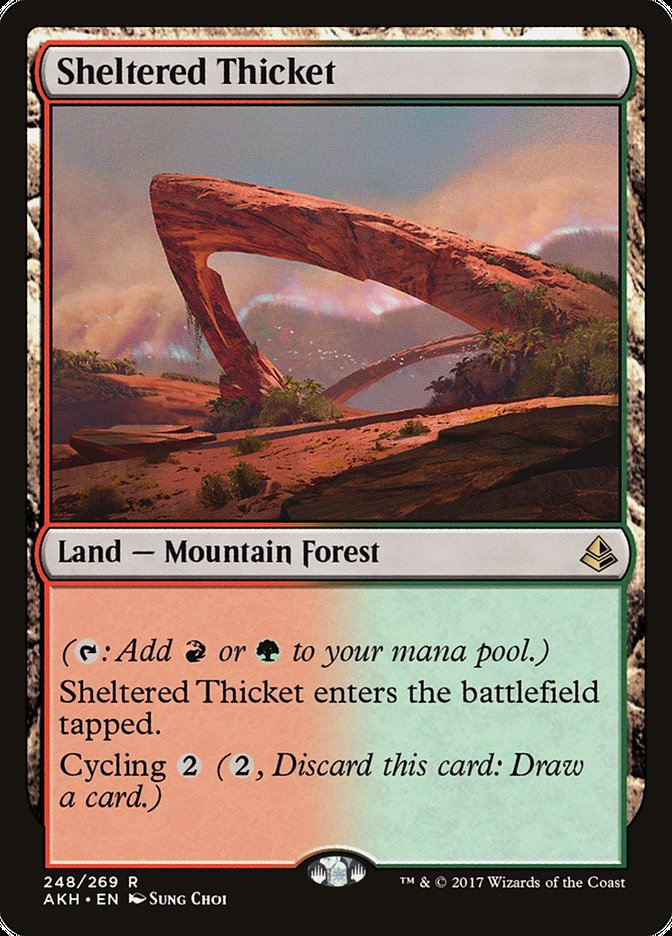
\includegraphics [width = 4cm, height = 6cm] {sheltered-thicket}
\end{center}
While generally played in classic RG lists as both card draw and an extra mana source, it presents both upsides and downsides over one of the canopy lands or \textbf{Tranquil Thicket}. Among its pros, we can obviously see that, being a fetchable land, allows us to have a better coloured manabase while providing extra utility in the long game. Its cons however are the fact that it is terrible in openers as a singular coloured mana source, and fetching it via fetchlands can prove problematic if one wants to use it as a source of card advantage.\\
\textbf{Verdict: Play 0-1}\\
\textbf{Total 4-6\\\\}
This puts us at a total of around 50 core pieces, depending on playstyle and personal preference, giving us plenty of room to splash.\\\\ Additional cards in green and colourless are considered below.\\\\
\newpage
\paragraph{Miscellaneous choices in G/colourless:\\}
While not essential to the deck, the following cards are very powerful and definitely worthy of maindeck consideration:\\\\
\textbf{Sylvan Library}
\begin{center}
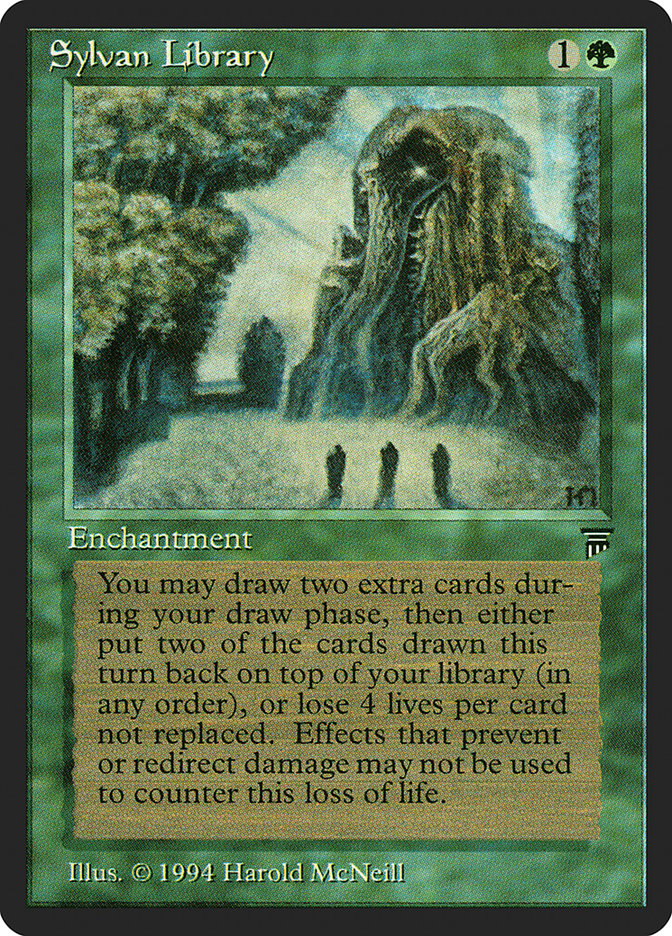
\includegraphics [width = 4cm, height = 6cm] {sylvan-library}
\end{center}
Allowing you to transform life into card advantage, Sylvan Library is a back-breaking turn 1 play against most fair decks, providing you with an easy way to get ahead of your opponents and stay ahead. Works great with Life from the Loam, as you can dredge for each draw, as long as a copy of Loam is present in the graveyard, without needing to put cards back, thus digging deeper for required lands.\\\\
\textbf{Crucible of Worlds\\}
\begin{center}
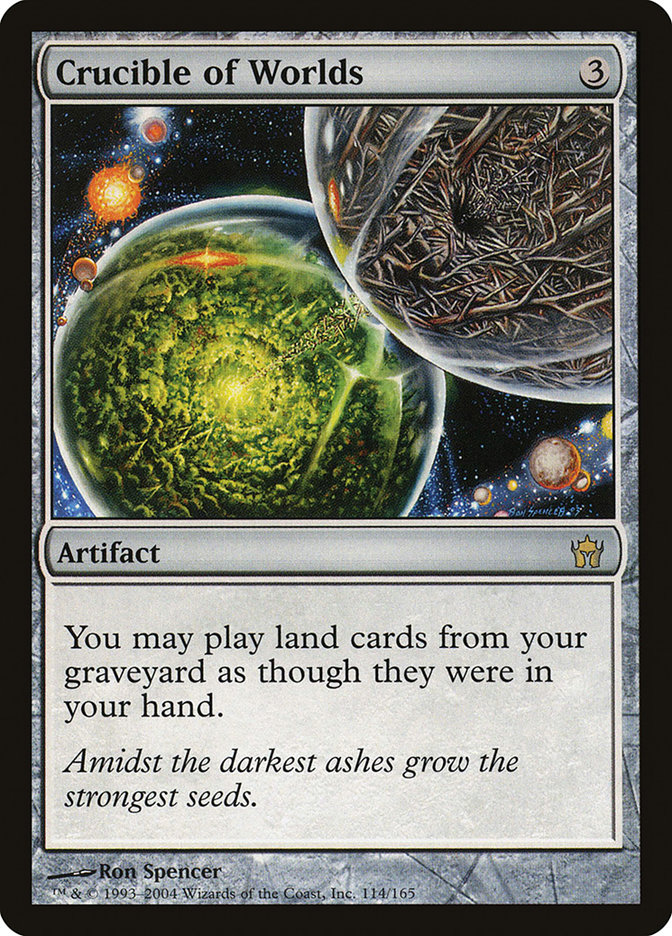
\includegraphics [width = 4cm, height = 6cm] {crucible-of-worlds}
\end{center}
Loam number 5, Crucible of Worlds is great in the matchups where Surgical Extraction can be expected. Sadly it does not dig for cards like Loam does, so it, while worthy of being in the 75, is not as good as Loam itself. Oko, Thief of Crowns adds insult to injury by turning it into an oversized land mammal. Still great in most matchups however.\\\\
\textbf{Engineered Explosives:}
\begin{center}
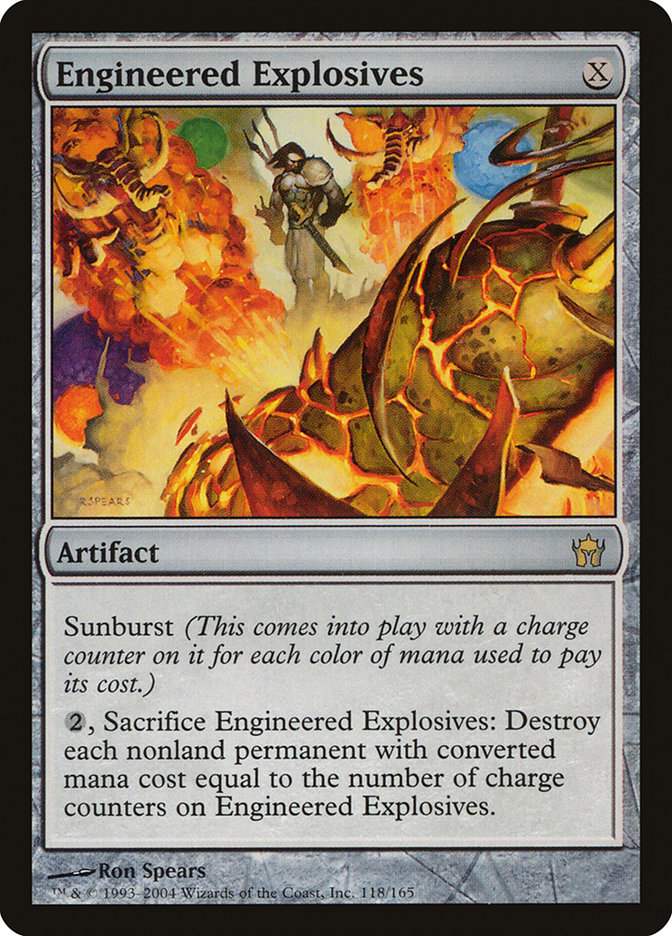
\includegraphics [width = 4cm, height = 6cm] {engineered-explosives}
\end{center}
A great colourless answer to problematic permanents like Oko, Thief of Crowns, Dreadhorde Arcanist and other high loyalty/toughness permanents, Engineered Explosives' utility is inversely proportionate to the number of colours being played. It is also weak to the increased countermagic present in the format, and can be rather mana intensive, as well as be mediocre in the face of Oko.\\\\
\paragraph{Sideboard Options:\\}
These cards instead either hose entire archetypes or easily swing the game in your favour and yet are generally too narrow to be played maindeck, however all of these have seen sideboard play at one time or another, most still do:\\
\newpage
\textbf{Elvish Reclaimer\\}
\begin{center}
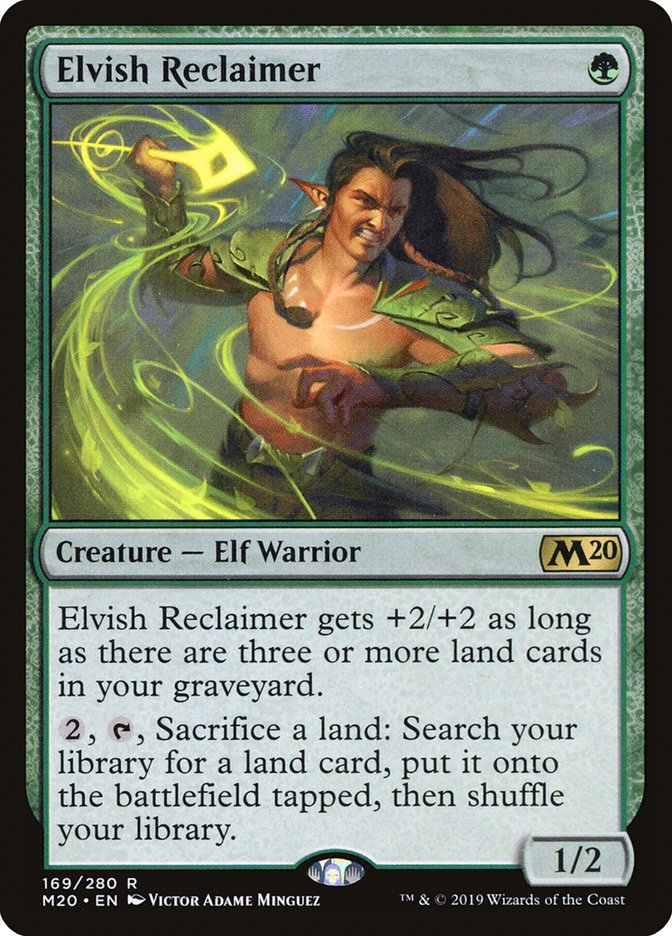
\includegraphics [width = 4cm, height = 6cm] {elvish-reclaimer}
\end{center}
A repeatable 2 mana crop rotation? I'm listening. And it becomes a sizeable clock with little to no mana investment? Sure, I'll take four!\\
Talk about the little elf that could!\\
While playing 4 is overkill, this card is very good. Its utility cannot be understated, as it\\
	-Gets any land we need, or the combo.\\
	-Can stonewall opposing creatures.\\
	-Is a relatively large clock.\\
	-Can easily be cast under Spheres.\\\\
This card generally supplants Tireless Tracker (see below) in many builds, as it is usually bolt proof too. Either are fine, it depends on personal preference. Usually played in \textbf{2-3 copies}\\\\
\newpage
\textbf{Tireless Tracker\\}
\begin{center}
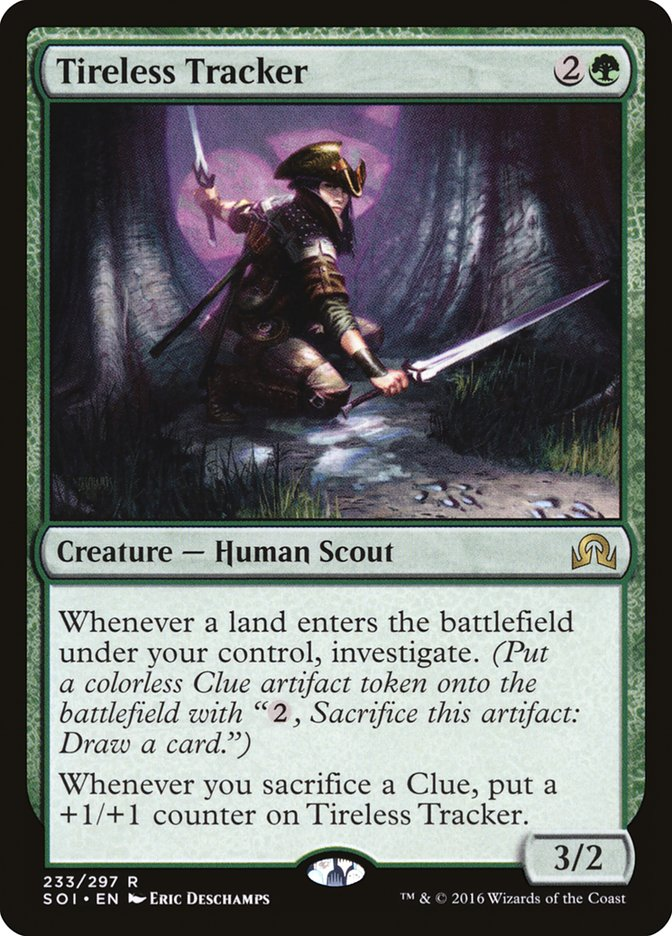
\includegraphics [width = 4cm, height = 6cm] {tireless-tracker}
\end{center}
Another all star Lands has gotten in the last 5 years, it transforms land drops into card advantage, all the while becoming a sizeable clock.\\While still a great card, its small body and its mana cost have contributed to its decrease in popularity of late, as \textbf{Field of the Dead} and \textbf{Elvish Reclaimer} largely substitute it in most lists.\\An excellent all around choice that gives Lands a win condition that does not depend on the graveyard. Usually played in \textbf{2-3 copies}.\\\\
\textbf{Choke\\}
\begin{center}
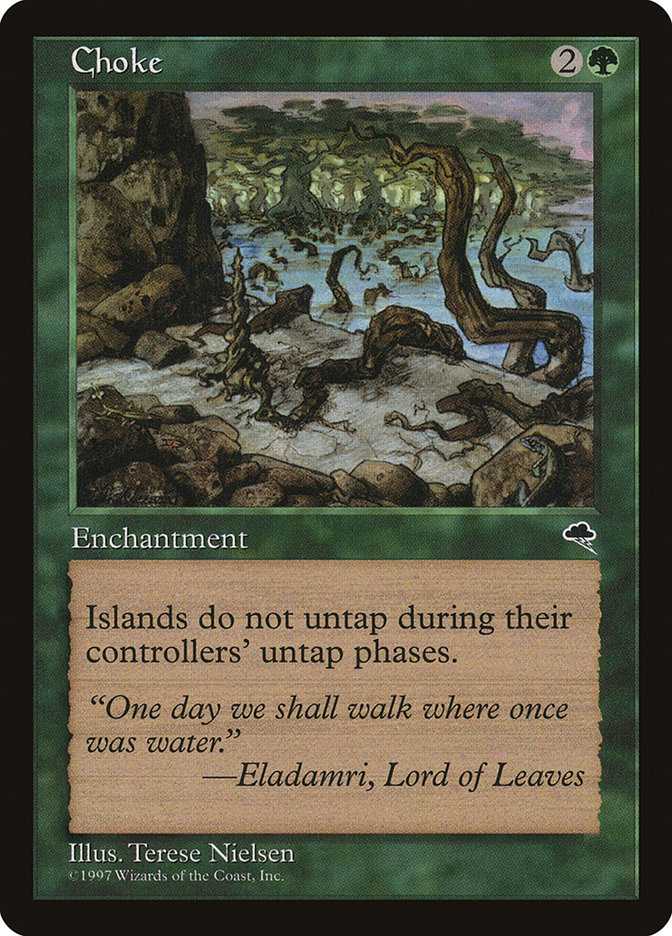
\includegraphics [width = 4cm, height = 6cm] {choke}
\end{center} Excellent hoser of the cantrip cartel, it punishes greedy blue decks and has great synergy with \textbf{Rishadan Port}. It is a must counter permanent that will greatly facilitate running away with the game upon resolution. Great against any blue heavy deck, which is a majority of the legacy metagame. Usually played in \textbf{2-3 copies}.\\\\
\textbf{Krosan Grip\\}
\begin{center}
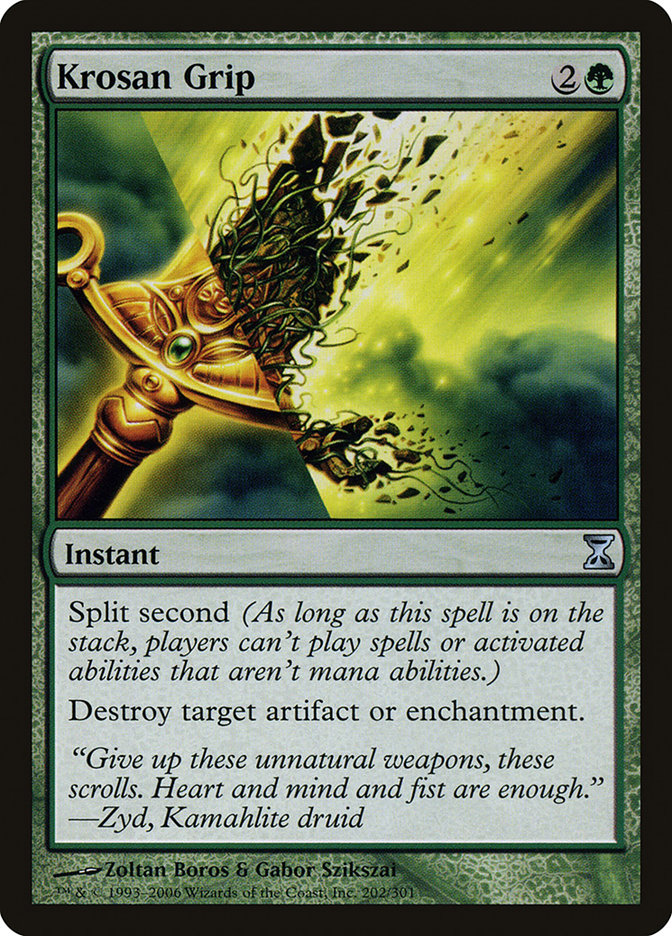
\includegraphics [width = 4cm, height = 6cm] {krosan-grip}
\end{center}A great card, however the Split Second effect has had less relevance since the departure of \textbf{Sensei's Divining Top}. Still great for hitting \textbf{Batterskull} and \textbf{Aether Vial}, as well as \textbf{Grindstone}, though the flexibility and relevative free cost of \textbf{Force of Vigor} (see below) somewhat outclasses it. Usually played in \textbf{1-3 copies\\}\\
\textbf{Force of Vigor\\}
\begin{center}
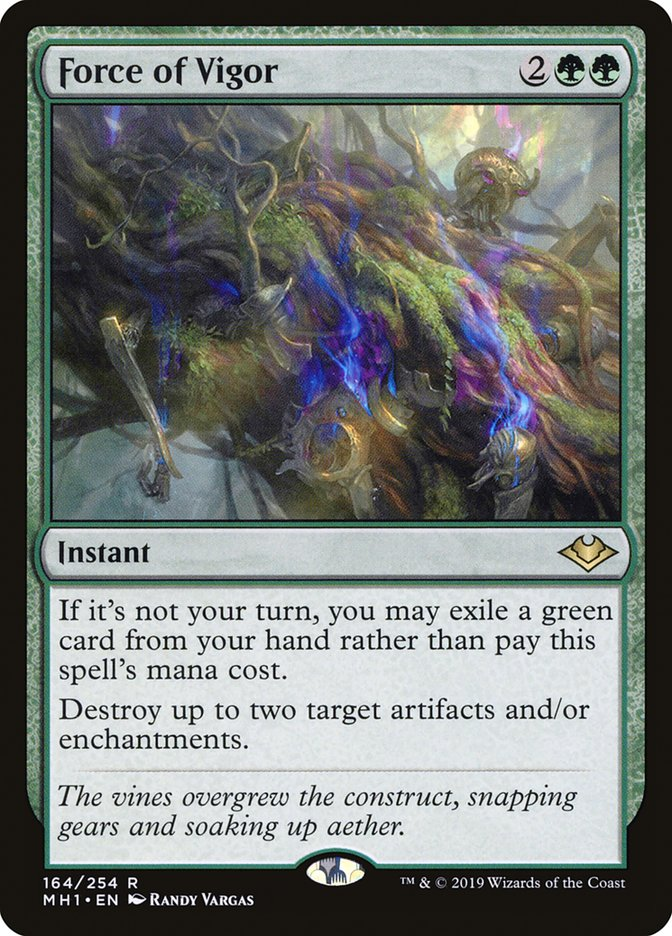
\includegraphics [width = 4cm, height = 6cm] {force-of-vigor}
\end{center}
Two for the price of one? And can be cast for free under a \textbf{Blood Moon}? Consider me convinced! This card is gas. It always being a 1 for 1 and often a 2 for 1 is very, very good, to a point that it has ousted Krosan Grip (card previously played in the sideboard) as the Enchantment/Artifact removal spell of choice. Great for dealing with \textbf{Blood Moon}, \textbf{Leyline of the Void}, \textbf{Back to Basics} and \textbf{Rest in Peace}, as well as pesky artifacts. An all around solid card from Modern Horizons.\\Usually played in \textbf{2-3 copies}.\footnote{Force of Vigor's alternate casting cost is worthless in the face of the Karn the Great Creator and Mycosynth Lattice lock, given that Mycosynth Lattice makes all cards colourless, hence the inability to exile a green card as part of the alternate casting cost of Force of Vigor.}\\\\
\textbf{Drop of Honey\\}
\begin{center}
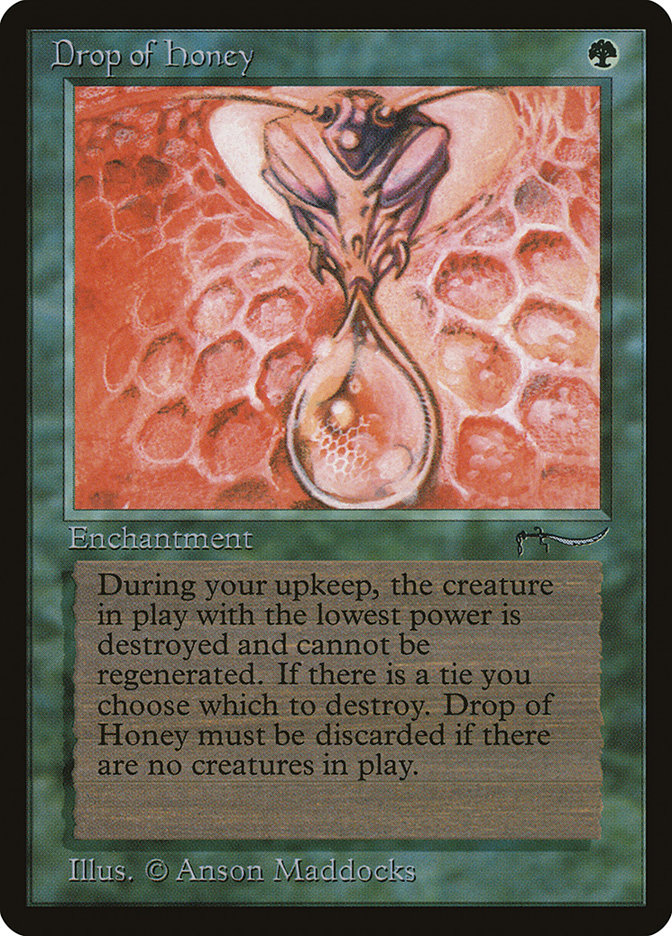
\includegraphics [width = 4cm, height = 6cm] {drop-of-honey}
\end{center}
This card, an old reference to the folktale "The Drop of Honey" from One Thousand and One Nights, a collection of Arabian fables, is a boon against creature heavy decks.\\For the low cost of one green mana, it continuously reduces the power on the battlefield, while at the same time impeding your opponent from committing further to the board.\\Coupled with Tabernacle and mana denial in the form of \textbf{Wasteland} and \textbf{Rishadan Port}, it can easily overwhelm opposing creature decks.\\Not played much until the printing of \textbf{True-Name Nemesis}, it is now generally considered stock in the sideboard as a way of keeping the battlefield clear as well as removing hard to remove threats like the aforementioned True Name Nemesis.Usually played in \textbf{1-2 copies}\footnote{Drop of Honey is expensive in paper, and while a valid choice in any Lands' player's sideboard, can easily be substituted by cards such as Kozilek's Return or Engineered Explosives if cost is a limiting factor.}\\
\newpage
\textbf{Veil of Summer:\\}
\begin{center}
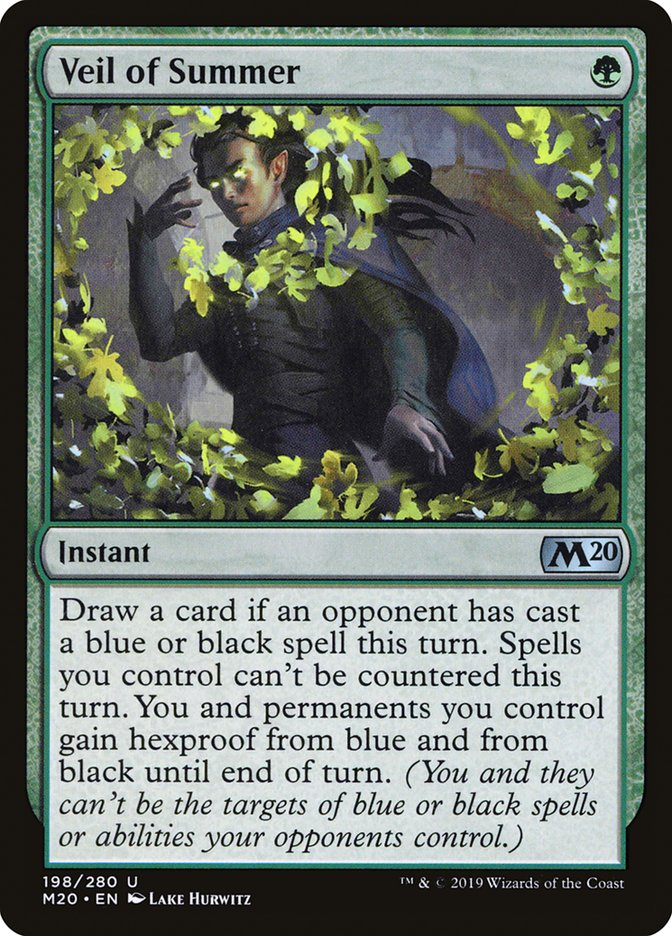
\includegraphics [width = 4cm, height = 6cm] {veil-of-summer}
\end{center}
\textbf{Pyroblast/Red Elemental Blast on steroids}, it makes \textbf{\emph{all}} of your spells uncounterable until EoT, as well as making you and your permanents hexproof from blue and black, and would be worthy of consideration on that alone.\\ However, it also \textbf{\emph{draws}} a card if an opponent has cast a blue or black spell in the turn it was cast. This card has so many applications, both reactive and proactive, it would require an article all by itself.\\Some important ones are as follows:\\\\
	-Veil allows you to force through lock pieces, like Chalice and Choke, against counter heavy decks, neutering their ability to play Magic.\\
	-Veil protects your permanents from Decay and Marit Lage from an Oko, Thief of Crowns +1 activation or a Brazen Borrower.\\
	-Veil protects your combo against Assassin's Trophy.\\
	-Veil protects you from discard, turning it into a 2 for 0 when played in response.\\
	-Veil protects your permanents from bounce spells like Vapor Snag and Hurkyl's Recall.\\
	-Veil protects Loam from Surgical Extraction; merely choose to dredge in response.\\
	-Veil protects Crop Rotations.\\
	-Veil protects you from Intuition and Predict, as well as Jace the Mind Sculptor.\\
This card is very powerful, and allows for some great proactive and reactive plays. Don't leave home without it. Usually played in \textbf{2-3 copies}.
\newpage
\textbf{Sphere of Resistance/Thorn of Amethyst/Chalice of the Void}
\begin{figure}
  \begin{subfigure}[b]{.325\textwidth}
\begin{center}
    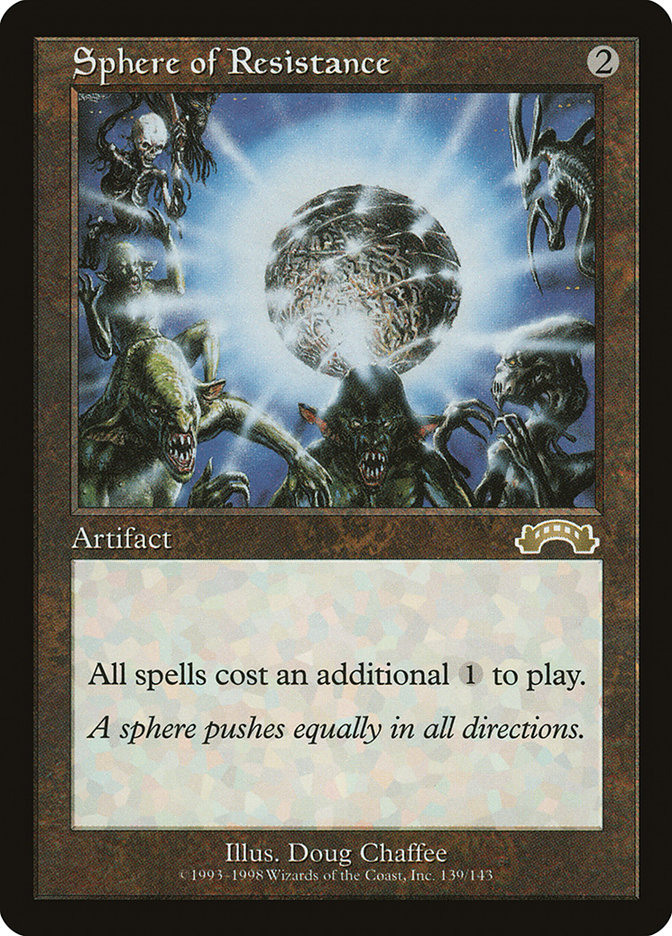
\includegraphics [width = 4cm, height = 6cm] {sphere-of-resistance}
    \caption{Sphere of Resistance}
    \label{fig:1}
\end{center}
  \end{subfigure}
  %
  \begin{subfigure}[b]{.325\textwidth}
\begin{center}
    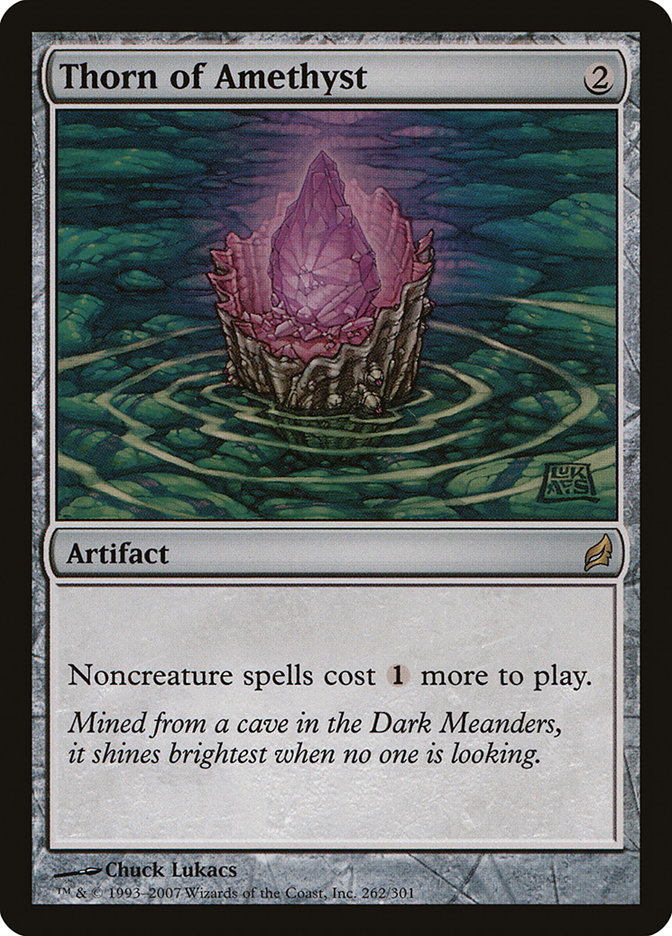
\includegraphics [width = 4cm, height = 6cm] {thorn-of-amethyst}
    \caption{Thorn of Amethyst}
    \label{fig:2}
\end{center}
  \end{subfigure}
%
  \begin{subfigure}[b]{.325\textwidth}
\begin{center}
    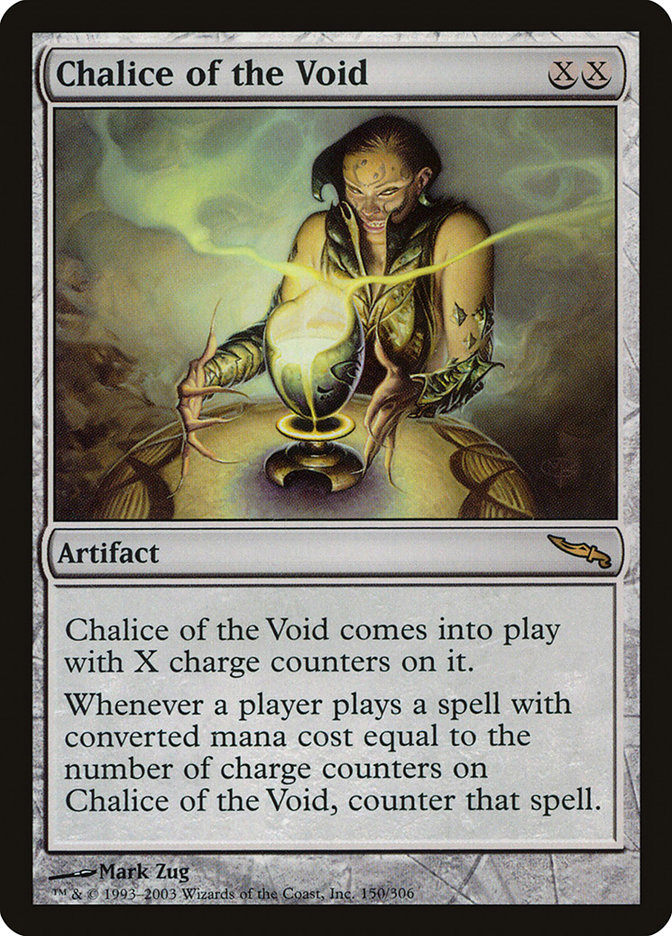
\includegraphics [width = 4cm, height = 6cm] {chalice-of-the-void}
    \caption{Chalice of the Void}
    \label{fig:3}
\end{center}
  \end{subfigure}
\end{figure}
\\\\This trio of cards make the faster combo matchups winnable, and are a necessity in a Lands sideboard. A split is fine, based on personal preference and taste, but playing any less than 4 total is a mistake. The card does serious work with Choke/Rishadan Port. \textbf{Sphere of Resistance} is usually always played in \textbf{4 copies}.\\Usually a \textbf{5th copy} of the effect is played as \textbf{Thorn of Amethyst}, however, \textbf{Chalice of the Void} has seen play as well, depending on personal taste.\\\\
\textbf{Nissa, Vital Force\\}
\begin{center}
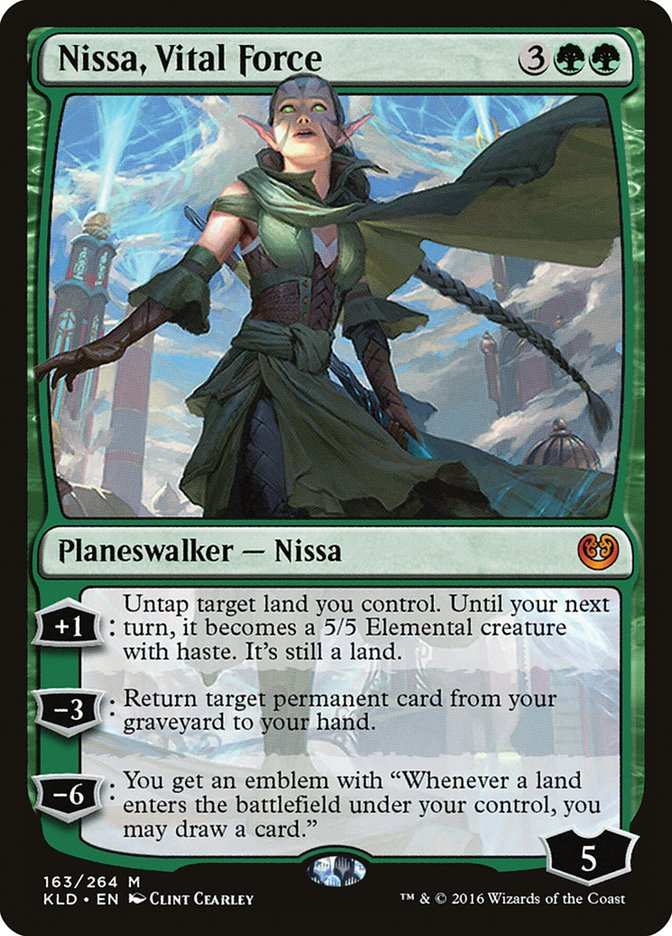
\includegraphics [width = 4cm, height = 6cm] {nissa-vital-force}
\end{center}
Such a great planeswalker in slower matchups, it makes for a fast clock as it can use its ultimate ability after one activation, where all of your land drops become redraws. Its + ability turns your lands into big 5/5 beaters, and its - ability returns any permanent to hand from the gy. So, what's not to like?\\
Its mana cost mainly. While being a huge counter magnet, it also is seriously outclassed by some of the other 2019 planeswalkers, like \textbf{Oko, Thief of Crowns} and \textbf{Karn the Great Creator}. When played, it is played in \textbf{1-2 copies}.\\\\
\textbf{Trinisphere\\}
\begin{center}
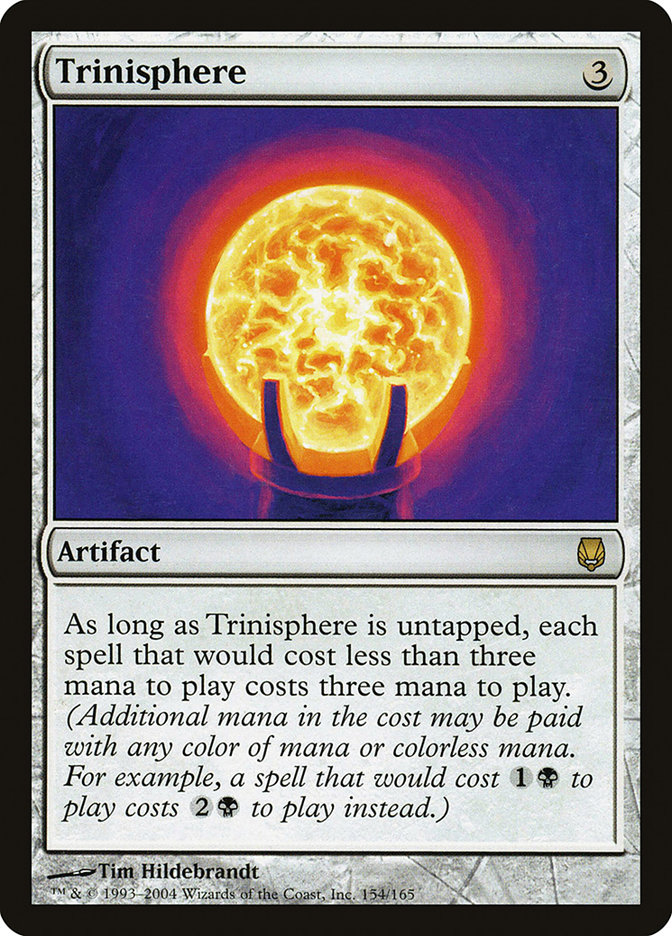
\includegraphics [width = 4cm, height = 6cm] {trinisphere}
\end{center}
Another powerful "sphere effect", it is a potential sideboard choice as a fifth sphere effect, similar to Chalice of the Void or Thorn of Amethyst , given both its synergy with classic sideboard staples such as Krosan Grip and Tireless Tracker, as well as Rishadan Port. In multiples it is quite bad however, and therefore usually only one is played, when it is chosent to be played.\\
Usually played in \textbf{0-1 copies}\\\\
\newpage
\textbf{Primeval Titan\\}
\begin{center}
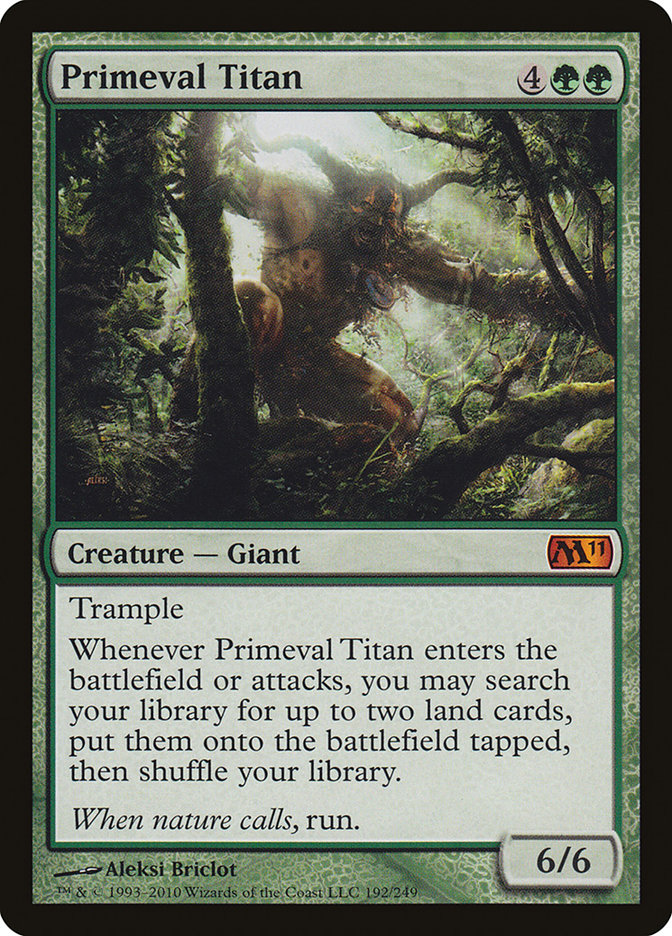
\includegraphics [width = 4cm, height = 6cm] {primeval-titan}
\end{center}
Once a worthy consideration in the SB, it had fallen out of favour until very recently, with the printing of \textbf{Field of the Dead}(and other cards), and is enjoying a bit of a resurgence. Now it is a very valuable card in fair matchups, as it can be easily ramped into, and provides value even if immediately removed. Titan is enjoying a resurgence in some unique Maverick-Lands hybrids, thanks also to the printing of \textbf{Dryad of the Ilysian Grove}, decks which have a playstyle very similar to the Amulet Titan deck from modern. When played, it is over (or alongside) \textbf{Elvish Reclaimer} or \textbf{Tireless Tracker} generally, and played in \textbf{1-2 copies}\\\\
\textbf{Boseiju, Who Shelters All\\}
\begin{center}
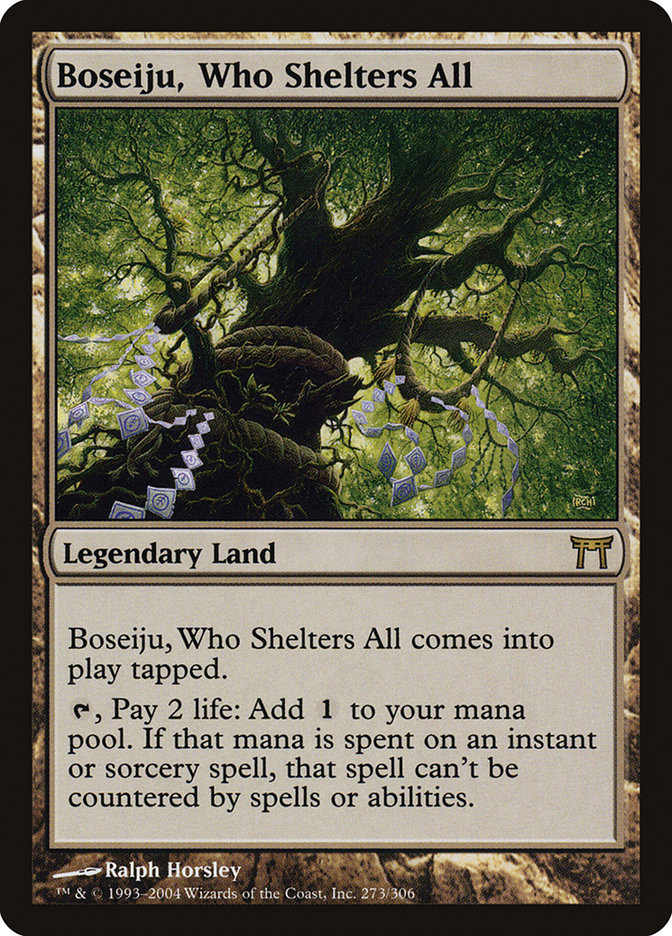
\includegraphics [width = 4cm, height = 6cm] {boseiju-who-shelters-all}
\end{center}
A relic of the past, this card used to be great against CounterTop decks, allowing for the casting of Loam even under a counterbalance lock, as they had no real way of dealing with it.\\ Nowadays, with the departure of \textbf{Sensei's Divining Top}, while still relevant in some matchups, \textbf{Field of the Dead} has taken its spotlight, as it is generally better in the matchups where you want Boseijiu.\\Still worthy of consideration, as Lands has ways of mitigating the life-loss, but there are certainly better options.\\The choice is up to you, it is very meta-dependent however.\\Usually played in \textbf{0-1 copies}.\\\\
\textbf{Warping Wail\\}
\begin{center}
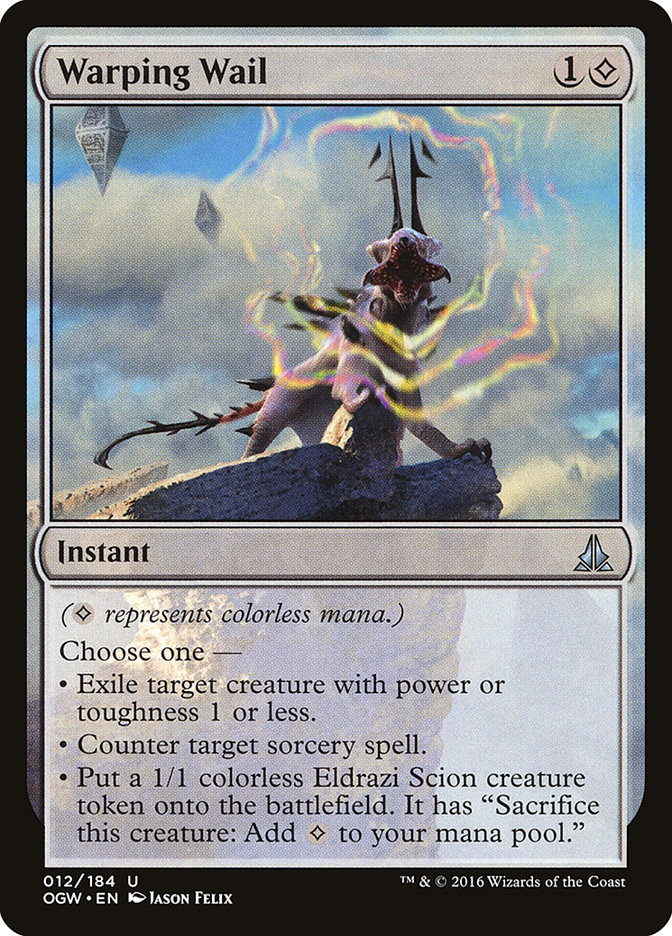
\includegraphics [width = 4cm, height = 6cm] {warping-wail}
\end{center}
Another new addition to our arsenal, it has surprising amounts of flexibility despite the narrowness in application it would seem to present, as it painlessly answers problematic cards such as \textbf{Dreadhorde Arcanist} as well as counters \textbf{Show and Tell}, two must answer cards. It also handily cleans up most of Death and Taxes creatures, as well as remove unflipped Delvers. Dependent on meta, it is usually played when combo is rampant.
Usually played in \textbf{0-1 copies}.\\
The preceding cards are the main choices available to green. More sideboard cards are available as colours are splashed and will be indicated in their respective sections.

\chapter{The Classic RG List}
This brings us to the traditional tried and true RG list, which uses the extra spots to splash for the following cards:\\
\textbf{Gamble\\}
\textbf{Punishing Fire} and \textbf{Grove of the Burnwillows}\footnote{(here, in this flavour, 3-4 of the 6 "untapped green sources" mentioned at the beginning are occupied by Grove of the Burnwillows for the combo with Punishing Fire)}\\
\textbf{Pyroblast/Red Elemental Blast and occasionally Molten Vortex\\}
As can be seen, the coloured mana base is split into\\
2 Taiga\\
3-4 Grove of the Burnwillows\\
1 Forest\\
3-5 Green Fetches (Verdant Catacombs, Misty Rainforest, Windswept Heath, Wooded Foothills)\\
That, together with Mox Diamond and our choice of canopy land, gives us around 14-17 untapped green sources, which is generally plenty to play all our spells.\\
Let's consider why the addition of red is so powerful, and also what made it unappealing (although definitely still viable) as time went on.\\\\
\newpage
\textbf{Gamble\\}
\begin{center}
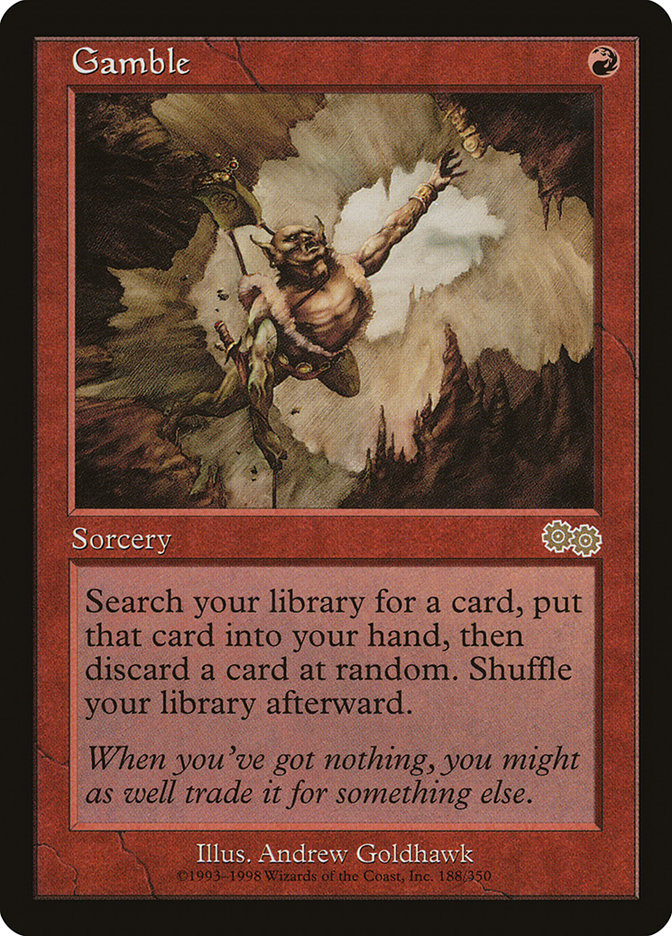
\includegraphics [width = 4cm, height = 6cm] {gamble}
\end{center}
While once an obligatory 3-4 of, the card has lost equity given the increase in speed of legacy compared to 5 years ago. Many cards have come and gone, and while still a pseudo one-mana \textbf{Demonic Tutor} in our deck, as its discard clause is rarely relevant (and can be lessened with proper sequencing), it no longer holds the privileged position it used to enjoy, given the increased density of counter magic and its weakness in games 2 and 3.\\Some versions of Lands even eschew Gamble all together for \textbf{Entomb} or card selection via \textbf{Sylvan Library}. Playing at least 2 copies is ideal if you have access to red, and I wouldn't personally go any lower. A great card, yet not as essential as before. \\
\textbf{Verdict: Play 2-4}\\\\
\textbf{Punishing Fire:\\}
\begin{center}
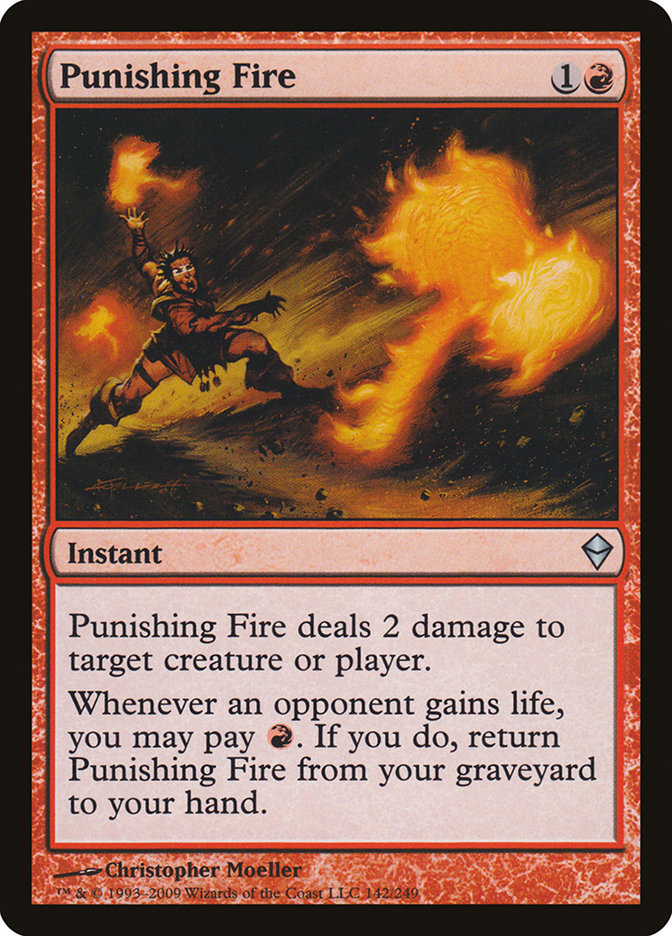
\includegraphics [width = 4cm, height = 6cm] {punishing-fire}
\end{center}
Oh, how the mighty have fallen. The once premier control card against creature strategies, plus allowing for a slow, sure wincon, it has all been "power crept" out of the format. Legacy has seen a large shift to creatures and planeswalkers with higher toughness and higher loyalty abilities, making 2 damage trivial.\\Among the "must kill" cards for Lands, \textbf{Wrenn and Six} (now no longer legal), \textbf{Dreadhorde Arcanist} and \textbf{Oko, Thief of Crowns}, have demonstrated the limitations of the 2 mana burn spell.\\Adding the exile clause on \textbf{Force of Negation} to the mix, and we can understand why Punishing Fire has lost some of the potency it once enjoyed. Still worthy of consideration, but recent innovations such as \textbf{Abrupt Decay} and \textbf{Oko, Thief of Crowns} have made it a secondary choice in the current meta.\\0-2 copies is sufficient in RGx, more in straight RG, as it is still the most synergystic removal spell available to straight RG.\\
\textbf{Verdict: Play 3-4}\footnote{1)When using Punishing Fire to deal with creatures that depend on the graveyard for their power and toughness (\textbf{Knight of the Reliquary}, \textbf{Tarmogoyf}), it is highly recommended to play Punishing Fire on the target first, and then \textbf{Crop Rotate} for \textbf{Bojuka Bog}, as this will avoid blowouts (especially relevant with the activated ability of \textbf{Knight of the Reliquary})\\
2) Be aware that since Grove of the Burnwillows is a mana ability, it can return Punishing Fire at any time, since it is a triggered ability. So even through Extirpate and split second effects.}\\\\
\textbf{Faithless Looting\\}
\begin{center}
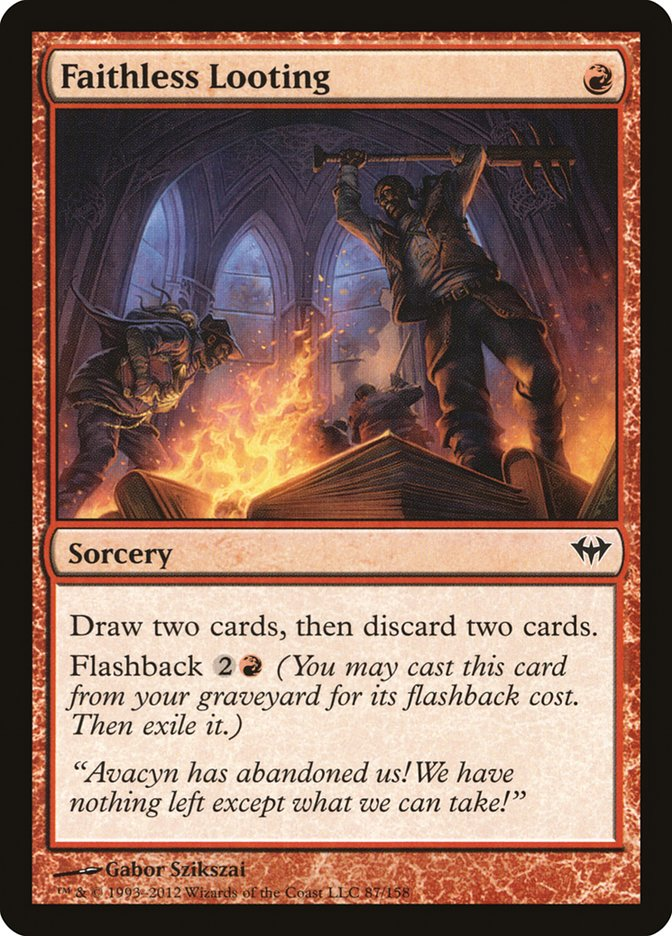
\includegraphics [width = 4cm, height = 6cm] {faithless-looting}
\end{center}
A viable alternative to Gamble, it has been played to some success in an attempt to make Lands less susceptible to discarding Gambled cards when such cards are not recurrable from the graveyard. A great way of digging through your deck, and finding key pieces, the flashback is only upside and works very well with an active Sylvan Library. Regardless, the card lacks the explosiveness of Gamble, as well as the efficiency the latter offers. Great in slower metagames with high numbers of grindy or control decks, it is worse in faster ones with lots of combo, so inclusion will hinge upon such. Decision of how many copies to play (or even if to include it in the main 60) are wholly left up to the pilot.\\\\
\textbf{Klothys, God of Destiny}
\begin{center}
\includegraphics [width = 4cm, height = 6cm] {klothys}
\end{center}
A very new addition to the Lands collection of played cards, Klothys has recently seen play as a ways of presenting a win condition without being reliant on the sideboard. Given its ability to exile cards from graveyards, it works as a slow method of removing problematic cards the aforementioned zone, in particular cards like \textbf{Uro, Titan of Nature's Wrath} or even opposing \textbf{Life from the Loam} or \textbf{Punishing Fire}. While too slow to provide efficient graveyard hate against faster decks that rely on the zone as a method of comboing off, it provides incremental value while being a nigh-unremovable win condition in slower, grindier matchups, in particular, Klothys can be backbreaking against slow control decks such as 4C Snowko.\\ Definitely worth of a slot in the maindeck or in the sideboard, depending on personal preference.\\\\
\paragraph{Sideboard:\\}
As already mentioned, Lands has gotten a series of cards that have been a boon to both the maindeck and the sideboard.
Cards typically played in the SB in RG (in addition to the previously mentioned green sideboard cards played across several colour combinations) are the following:\\\\
Pyroblast/Red Elemental Blast\\
Cindervines\\
Ancient Grudge\\
Molten Vortex\\
Chandra, Awakened Inferno\\
Boil\\
Kozilek's Return\\
Faithless Looting\\\\
\textbf{Pyroblast/Red Elemental Blast\\}
\begin{center}
\includegraphics [width = 8cm, height = 6cm] {pyroblast-reb}
\end{center}
A great sideboard tool, as it helps fight through countermagic and, more importantly, destroys \textbf{Oko, Thief of Crowns}, as well as gets rid of \textbf{Back to Basics} and deals with \textbf{True Name Nemesis} on the stack.\\Arguably the main reason to be on Red currently, together with the flexibility of Gamble. Worthy of a couple sideboard spots, as it deals with many problematic cards. Usually played in \textbf{0-2 copies}.\\\\
\textbf{Cindervines\\}
\begin{center}
\includegraphics [width = 4cm, height = 6cm] {cindervines}
\end{center}
A relatively recent edition, it sees play as both a hedge against Storm based combo decks, while providing outs to pesky enchantments and artifacts that may hinder our gameplan. \\Recently it has seen less play in favour of \textbf{Force of Vigor}. \\Usually played in \textbf{0-2 copies}.\\\\
\textbf{Ancient Grudge\\}
\begin{center}
\includegraphics [width = 4cm, height = 6cm] {ancient-grudge}
\end{center}
An old piece of tech from the past, generally is superseded by better options (mainly \textbf{Force of Vigor}), as its inability to destroy enchantments is a huge negative. Valuable in metas with lots of 12 Post or Eldrazi Prison or any deck that plays a large amount of artifacts. Decent also against Death and Taxes for equipment, \textbf{Aether Vial} and \textbf{Phyrexian Revoker}. Usually played in \textbf{0-2 copies.}\\\\
\textbf{Molten Vortex}
%\footnote{The legacy lands discord player Barcode has stated (and I quote) the following: "yeah Molten Vortex is still bad ;)" Consider such when choosing which cards to play.}
\begin{center}
\includegraphics [width = 4cm, height = 6cm] {molten-vortex}
\end{center}
The red removal spell of choice for larger creatures in classic RG builds, its mana intensive activation works against its adoption however, as it has a hard time of killing high toughness creatures or high loyalty planeswalkers due to the few red sources the deck fields. Some lists play it maindeck, some bring it in as a flexible sideboard option against creature decks as an additional hedge alongside Tabernacle. Usually played in \textbf{0-2 copies}\\\\
\textbf{Chandra, Awakened Inferno\\}
\begin{center}
\includegraphics [width = 4cm, height = 6cm] {chandra-awakened-inferno}
\end{center}
This recent addition to the pool of sideboard choices wreaks havok on Ux/Uxx decks, as its uncounterability together with its ability to keep the board clear via its -3 and present a very fast clock via its +2 (along with its ultimate) make for a potent combination against decks that traditionally have difficulty answering planewalkers. A must in control heavy metas.Usually played in \textbf{0-2 copies}\\\\
\newpage
\textbf{Boil\\}
\begin{center}
\includegraphics [width = 4cm, height = 6cm] {boil}
\end{center}
Another blast from the past, it is game-winning when coupled with \textbf{Boseiju, Who Shelters All}. Destroying all of your opponent's islands is not to be underestimated in a format rife with blue mana such as Legacy is.\\Often played in sideboards that play a Burning Wish package, it is a powerful tool once again in metagames in which blue decks are highly represented, that however has somewhat dropped off in favour of more impactful cards.Usually played in \textbf{0-2 copies}\\\\
\textbf{Kozilek's Return\\}
\begin{center}
\includegraphics [width = 4cm, height = 6cm] {kozileks-return}
\end{center}
A great sweeper, especially against go wide strategies, its most important application is the ability to get around protection given from \textbf{Mother of Runes} out of Death and Taxes and Maverick/Junk style decks, thanks to the keyword Devoid. While \textbf{Drop of Honey} is favoured as its ability gets around power and toughness, this is a perfectly valid substitute. Usually played in \textbf{0-2 copies}\\\\
Having concluded our sideboard options (there are many others, but herein are listed the most common ones) let us take a look at a sample decklist and some opening hands, and assess them in the following section.\\
\paragraph{Sample List and Hands:\\\\\\}
A typical decklist looks as follows\footnote{Taken from Freya Sanford's \emph{Leaving a Legacy Open VI, 1st Place List, 02/02/2020}; slight changes are made to the sideboard.}:\\\\
\begin{center}
\textbf{Maindeck}
\includegraphics [width =\textwidth] {rgdecklist1}
\includegraphics [width =\textwidth] {rgdecklist2}
\includegraphics [width =\textwidth] {rgdecklist3}
\end{center}
\begin{comment}
Maindeck:\\
4 Wasteland\\
2 Taiga\\
1 Forest\\
3 Rishadan Port\\
4 Thespian's Stage\\
4 Dark Depths\\
2 Maze of Ith\\
4 Grove of the Burnwillows\\
1 Windswept Heath\\
1 Wooded Foothills\\
1 Verdant Catacombs\\
1 Misty Rainforest\\
1 The Tabernacle at Pendrell Vale\\
1 Bojuka Bog\\
1 Sheltered Thicket\\
1 Field of the Dead\\
1 Blast Zone\\
1 Ghost Quarter\\
1 Nurturing Peatland\\
1 Horizon Canopy\\
4 Mox Diamond\\
4 Exploration\\
1 Manabond\\
4 Crop Rotation\\
2 Gamble\\
4 Life from the Loam\\
3 Punishing Fire\\
2 Sylvan Library\\\\
Sideboard:\\
1 Krosan Grip\\
2 Force of Vigor\\
4 Tireless Tracker\\
4 Sphere of Resistance\\
2 Choke\\
2 Pyroblast\\
\end{comment}
\begin{center}
\textbf{Sideboard}
\includegraphics [width =\textwidth] {rgdecklistsb}
\end{center}
Let us now take a look at some sample hands. For sake of simplicity, we will consider all hands as being on the play (unless indicated otherwise).\\
\begin{center}
\textbf{Hand 1\\}
\includegraphics [width =\textwidth, height = 3cm] {rghand1}
\end{center}
This hand is rather bad. While we have all our heavy hitters, between answers to creature decks with Punishing Fire and Tabernacle, a way to dig for combo/utility lands with Sylvan Library and Crop Rotation, and Life from the Loam, our engine, we have little coloured mana, no acceleration, and can't cast anything. We have better sixes, especially with the London mulligan, at our disposal.
\begin{center}
\textbf{Mulligan N°1\\}
\includegraphics [width =\textwidth, height = 3cm] {rgmull1}
\end{center}
This hand is great, a snap keep. We have our engine card, ways to cast it, and effectively the combo in hand between Crop Rotation and Dark Depths. The hand may be slightly soft to creature decks, but access to go wide or go tall strategies are rectified by Tabernacle or Maze of Ith, both which can be found off of Crop Rotation if needed. 
Card to put back: Grove of the Burnwillows.
\begin{center}
\textbf{Hand 2\\}
\includegraphics [width =\textwidth, height = 3cm] {rghand2}
\end{center}
An excellent hand. We have acceleration via Mox Diamond and Exploration, Life from the Loam in hand thanks to Gamble, and Maze of Ith for creature decks or Rishadan Port for combo. The hand is rather soft to fast combo, as well a counter on Gamble (which can be baited out by playing Exploration).\\
\begin{center}
\textbf{Hand 3\\}
\includegraphics [width =\textwidth, height = 3cm] {rghand3}
\end{center}
The hand is slow, and definitely keepable in known matchups. I'd err on the side of keep, especially in a world with Force of Negation, as we have two Loams in hand as a safeguard against it. Punishing Fire, though lacking Grove, is good for the first couple turns while we dig with Loam. Rishadan Port also works in our favour against combo decks, and Misty Rainforest ensures mana stability. I would keep, even more so on the draw.
\newpage
\begin{center}
\textbf{Hand 4\\}
\includegraphics [width =\textwidth, height = 3cm] {rghand4}
\end{center}
This is a classic example of a hand that looks great, but is in fact terrible. This is because of 2 things principally:
\\1) Do not keep hands that ramp into nothing. This seven looks great at a first glance, but at a closer look e can't fight off creature decks adequately, as we have Grove but no Punishing Fire, (Crop Rotation for Tabernacle is decent, but then we throw away our ability to assemble the combo should we find either Thespian's Stage or Dark Depths) and we have no way of assembling nor digging for Life from the Loam. We have Exploration, which is always ideal in an opener, but we can't abuse it without Life from the Loam.
\\2)Do not keep hands that have no way of finding Life from the Loam. 
It cannot be overstated how essential Life from the Loam is (at least in G1) and finding it should be a pilot's utmost priority. This hand presents no way to assemble the engine, and as such cannot be considered in the blind. An easy mulligan.
Note: If the 7 card hand had Thespian's Stage over say, Ghost Quarter, this hand becomes very very good in certain matchups, mainly combo ones, as it allows us to assemble the combo very quickly while staving them off, which is the best the deck can do in faster matchups, where it suffers. By switching Ghost Quarter for Thespian's Stage, so the hand becomes:
\begin{center}
\textbf{Hypothetical Hand\\}
\includegraphics [width =\textwidth, height = 3cm] {rgmull2}
\end{center}
We now can play out Mox Diamond pitching Grove of the Burnwillows, play Exploration with Mox, play Rishadan Port and Thespian's Stage and threaten to combo off the next turn with Wasteland. The hand is rather all in, but such hands can be very good against fast combo decks like Reanimator and Storm, where Lands suffers.
\newpage
\begin{center}
\textbf{Mulligan N°1\\}
\includegraphics [width =\textwidth, height = 3cm] {rgmull3}
\end{center}
This six is decent, as we can put back a Punishing Fire, have enough mana to cast all our spells, and can dig for Loam with Sylvan Library. A bit on the slow side, but definitely a keepable hand. Tabernacle and Maze of Ith help us against creature decks, though we'll have to make a choice between the two. Personally I'd keep Maze of Ith and discard Tabernacle, as Maze of Ith and Punishing Fire allows us to deal with 2 creatures with more ease in comparison to Tabernacle and Punishing Fire.\\\\\\
This concludes the part regarding the classic RG list.\\
However, the Legacy metagame is rife with change compared to even 3 months prior to the writing of this primer. The format is in constant flux, and the appearance of \textbf{Wrenn and Six}, \textbf{Dreadhorde Arcanist}, \textbf{Oko, Thief of Crowns}, \textbf{Force of Negation} and \textbf{Brazen Borrower} just to name a few have made straight, combo focused RG, unappealing in general. Answers were looked for, and found. Innovation, new card printings and the reworking of lists and manabases as a whole caused the archetype to splinter in different flavours/colours, which can be mainly classified in order of popularity as follows:\\\\
\textbf{RG, RGB (Jund), BUG (Sultai), UG, RUG (Temur)}\\
Note to the reader: Make NO mistake, the classic RG list is very, very good. It is perfectly capable of performing at the highest levels in the hands of a skilled pilot, and is a great choice for any tournament, and is the go to list for any Lands player.\\
This part of the primer seeks merely to update the changes occuring to the Lands archetype as a whole, and explain what spurred on these changes, all the while gathering the various evolutions of the deck in one place as well as making them more easily accessible.\\\\
Before getting into the other colour pairings Lands players have turned to, I want to now assess the cards which brought about such change.
\chapter{2019 Metagame Changes: Part One}
\textbf{Wrenn and Six\\}
\begin{center}
\includegraphics [width = 4cm, height = 6cm] {wrenn-and-six}
\end{center}
Without a doubt, one of the single most influential cards (though there are several) the archeype has received (and Legacy as a whole, during its legality), was Modern Horizon's 2019 printing of the exceptionally powerful planeswalker (arguably most powerful of its type up to that point) Wrenn and Six.
This card, absolutely devasting in RUG Delver\footnote{To put the importance of Wrenn and Six to RUG Delver in perspective, RUG Delver often played a couple Life From the Loams themselves in the sideboard against Wasteland decks, as their manabase was exceptionally weak to nonbasic land hate prior to the two-mana planeswalker. Wrenn and Six gave them both a source of repeatable removal and a way of winning the long game, as well as a continuous source of card advantage, both unheard of in tempo decks like delver.}  lists, was responsible for the demise of several longstanding legacy archetypes. While many decks, such as Death and Taxes, Elves and Goblins, suffered from the repeatable removal granted by its -1 ability, classic RG Lands, which hinges on mana denial through Wasteland and Rishadan Port, could simply not keep up with the low to ground, powerful threats presented by RUG Delver backed up by a plethora of countermagic.\\ 
Many decks, previously preying on the fragility of RUG Delver's manabase, could no longer do so thanks to the effective "draw a card" clause Wrenn and Six's +1 presented, as a Delver player could simply opt to return destroyed lands to hand, instead of needing to churn through the deck to find them.\\
This, in addition to giving Delver a way of turning their Wastelands, commonly used as tempo plays, into win conditions, proved to be too much for many decks of the format. Naturally, Wrenn and Six is mediocre against Lands by itself, as it can simply be steamrolled via Exploration, but when paired with a clock such as Delver of Secrets or Tarmogoyf and free countermagic, could threaten to overrun Lands with ease, thanks to its +1 ability and rather high loyalty, previously unseen on such a cheap planeswalker.\\
RUG Delver, being the monstrosity of efficiency that it was, presented, between Wrenn and Six, and War of the Spark's Dreadhorde Arcanist, a series of extremely powerful card advantage engines (arguably its namesake card, Delver of Secrets, is nowadays the worst, although still very good, card in a deck full of hyper-efficient threats), backed by Force of Negation and the increased density of countermagic (another printing from Modern Horizons) as well as efficient beaters in Tarmogoyf and Delver of Secrets, required answers to threats Punishing Fire was no longer able to satisfy.\\
Thus, amid Lands playing its own Wrenn and Sixes, the first innovation was born, the black splash for Abrupt Decay, with Leyline of the Void in the sideboard, as ways of dealing with both threats from different angles of attack (removal and mass graveyard hate).\\
However, Wrenn and Six wasn't the only reason for the move towards black. Infact, reinforcing the black splash and pushing RG Lands even further to a RBG (Jund) colour pairing, were the aforementioned cards Dreadhorde Arcanist (War of the Spark) and Force of Negation (Modern Horizons). This is the reason black continues to be played as a splash colour of choice even after Wrenn and Six's banning on Novermber 18th, 2019.\\\\
\newpage
\textbf{Dreadhorde Arcanist\\}
\begin{center}
\includegraphics [width = 4cm, height = 6cm] {dreadhorde-arcanist}
\end{center}
This card, while seemingly innocent (and mostly so in formats with younger card pools such as Modern and Pioneer), when played alongside powerful 1 mana instant and sorcery spells like Brainstorm, Lightning Bolt, Ponder, Preordain in Legacy (Ancestral Recall and Gitaxian Probe in Vintage, where it was right at home in Jeskai/RUG "Xerox" decks) very easily spirals out of control. This, coupled with the fact that its 3 toughness made it very difficult to kill in the face of countermagic, was a second reason to consider the black splash, as Abrupt Decay provided an easy answer to it. Dreadhorde Arcanist, when played alongside format staples such as Lightning Bolt, Ponder and Brainstorm,  is easily the best threat in URx Delver lists even today, and will likely remain so for the forseeable future. \\\\
\textbf{Force of Negation\\}
\begin{center}
\includegraphics [width = 4cm, height = 6cm] {force-of-negation}
\end{center}
The final nail in the coffin, the third of the trifecta out of RUG Delver represented by Wrenn and Six, Dreadhorde Arcanist and Force of Negation, Force of Negation easily prevented chaining of Punishing Fires to kill the former two cards, while also stopping our engine in Life from the Loam thanks to its exile clause, necessitated the adoption of better answers, such as Abrupt Decay, a desirable choice thanks to its uncounterability \\
Abrupt Decay has since been a staple in some Lands builds, allowing for the quick and painless removal of otherwise troublesome cards like Knight of the Reliquary and Monastery Mentor, as well as remove graveyard hate in post sideboard games. The card is an all star in many matchups, thanks to its catch-all nature.\\
The black splash however, was not only for Abrupt Decay. Dreadhorde Arcanist and Wrenn and Six, having become both enemy number one in a metagame dominated by RUG delver, also encouraged the adoption of Leyline of the Void, as its "uncounterable" put into play ability ensures no graveyard recursion from either Arcanist or Wrenn, as well as keeping Tarmogoyfs somewhat small, prior to its removal\\
This brings us to the first evolution, albeit small, to the archetype, the RBG/Jund build.
\subsection{Dark (Jund) Lands}
Arguably as popular as the classic RG build nowadays, it makes a small black splash for \textbf{Abrupt Decay} in the maindeck and \textbf{Leyline of the Void} in the sideboard plus access to general purpose black sideboard cards, including but not limited to \textbf{Surgical Extraction} and \textbf{Plague Engineer}.\\
Long has the black splash been known as of potential interest, given access to such card engines like Dark Confidant (nearly without drawback in a deck with such few spells), and yet, the following list of cards are what is usually played today:\\
not much has changed, as the general card suite and land selection is mainly unchanged across flavours, but the black spash opens up several new maindeck and sideboard options to the deckbuilder)\\\\
\textbf{Abrupt Decay\\}
\begin{center}
\includegraphics [width = 4cm, height = 6cm] {abrupt-decay}
\end{center}
Often regarded as one of the best removal spells ever printed, Abrupt Decay cleanly and effortlessly answers a host of permanents that cannot be easily removed through damage (like \textbf{Knight of the Reliquary}, \textbf{Tarmogoyf} or \textbf{Oko, Thief of Crowns}), or are simply not creatures, without fear of being countered. A surgically precise tool to remove the smorgasbord of "must kill" permanents 2019 has brought to Magic as a whole, it improves our Delver matchup, as it is a surefire way to remove troublesome permanents even through countermagic\\ As a side bonus, it can also remove graveyard hate cards like \textbf{Rest In Peace} or non basic land hate like \textbf{Back to Basics} or \textbf{Blood Moon}. However, the inability to be recurred, despite being a fast answer to most threats, can make dredging Loam worse, especially when looking for answers. Thanks to this, it is often ideal in openers given also that it seeks to answer threats generally played the first couple turns of the game. In decks that black it as a black splash, generally 2-3 copies are played between the maindeck and the sideboard, accompanying 1-2 copies of Punishing Fire.\\
\textbf{Verdict: Play 2-3 copies.\\\\}
\textbf{Entomb\\}
\begin{center}
\includegraphics [width = 4cm, height = 6cm] {entomb}
\end{center}
The black splash gives us some alternatives over Gamble in looking for Loams, and while Entomb is somewhat narrower, as we cannot use it to find some non recursive spells like \textbf{Exploration} or \textbf{Crop Rotation}, differently from Gamble, it still has incredible synergy with a large majority of our deck. An instant speed tutor, it allows us to play a more reactive game in certain matchups, where this is especially important in post-sideboard games. While comparable to Gamble, usually the latter is favoured, as tutoring to hand can often be game-winning in certain matchups where specific hate is needed as soon as possible.\\
\textbf{Verdict: Play 2-3}, similarly to Gamble.\\\\
\textbf{Sideboard Choices:\\}
The sideboard choices are where the choice to play black really shine, as we get to play the following cards:\\
Note: The following cards are merely potential options in black. They are not to be played all together, but a mix and match of cards and their respective quantities, developed through playtesting and personal preference depending on playstyle, is heartily encouraged. I have only listed a suggested amount of copies as a mere suggestion; final numbers and card distribution are wholly up to the pilot's taste.\\\\\
\textbf{Leyline of the Void\\}
\begin{center}
\includegraphics [width = 4cm, height = 6cm] {leyline-of-the-void}
\end{center}
A no brainer, as completely turns off the graveyard for free, provided it is present in openers. With the London Mulligan, finding it in the initial has never been easier, and is an obvious sideboard choice against decks like Bx Reanimator, ANT and Dredge/Hogaak in addition the the Delver decks playing \textbf{Dreadhorde Arcanist} and \textbf{Wrenn and Six} (RUG) or \textbf{Dreadhorde Arcanist} and \textbf{Gurmag Angler} (Grixis), or any deck (Stryfo Pile being a good example) that seeks to leverage the graveyard.\\ Leyline of the Void is also a decent choice against \textbf{Knight of the Reliquary} decks like Maverick and 4C/5C Loam as well as a natural choice in the mirror. Coupled with \textbf{Abrupt Decay}, it improves several matchups  (Delver being the main one) considerably while making our hardest matchup, Sneak and Show, worse, thanks to the number of sideboard slots it requires to make it worthwhile. Usually played in 4 copies.\\
\textbf{Verdict: Play 4 copies.\\}
\textbf{Surgical Extraction\\}
\begin{center}
\includegraphics [width = 4cm, height = 6cm] {surgical-extraction}
\end{center}
Surgical Extraction is another form of graveyard hate, but instead of completely removing the graveyard (continuous, as Dice calls it in his Lands primer, see link to the source), it removes a single target from the graveyard and library, at instant speed, and is "free". A great choice in the faster graveyard matchups like Bx Reanimator, it is bad in the face of Delver and decks that seek to use the graveyard as a resource rather than a combo element. Still, its flexibility merits consideration. It can be very good in the Lands mirror, though good players will play around it.
Usually played in 1-2 copies.\\
\textbf{Verdict: Play 1-2 copies.\\\\}
\textbf{Plague Engineer\\}
\begin{center}
\includegraphics [width = 4cm, height = 6cm] {plague-engineer}
\end{center}
This infamous card is the bane of many tribal and white weenie strategies, from Elves to Goblins to even Death and Taxes, and walks the fine line between "exceptionally powerful" and "format-warping". This card is mainly responsible for the drop-off of the aforementioned decks (except Death and Taxes, to which it still is very unkind) and, when played in the Wrenn and Six era, all but spelled certain death for small creature strategies. Plague Engineer, still enjoying considerable play today, as it is almost always a 2 for 1, is the reason Stoneblade decks are enjoying less play as well, as it kills their most efficient beater, \textbf{True-Name-Nemesis}. A great card for dealing with Dreadhorde Arcanist as well, as Arcanist's ability is rendered null by the loss in power, it also trades up quite effectively and can stonewall opponents creatures.
A very good choice for the modern Legacy meta, especially in creature/tribal heavy metagames.\\
\textbf{Verdict: Play at least 2} if played.\\\\
\textbf{Dark Confidan:\\}
\begin{center}
\includegraphics [width = 4cm, height = 6cm] {dark-confidant}
\end{center}
Dark Confidant, affectionately titled "Bob" after its designer Bob Maher, being the multiformat staple that it is, is definitely worthy of consideration in a deck whose average converted mana cost is around .7 to .8. The card can easily represent an easy source of card advantage indepently of the graveyard, while still offer a decent means of clocking our opponent and eventually reducing their life total to 0.\\ Already played to great effect in 4C Loam, whose abundance of lands (usually around 27) means that life loss from the extra cards is relatively low which is true even more so in Lands, as we have a lower mana curve. The card had fallen out of favour in the Wrenn and Six era and still has not enjoyed much of a resurgence, however it shines in control heavy metas.\\ Works wonders alongside \textbf{Sylvan Library}, as one can fix their draws as to essentially never lose life off of Bob. A good sideboard choice for the Jund flavour of Lands.\\
\textbf{Verdict: Play 2-3 copies} if played.\\\\
\newpage
\textbf{Thoughtseize\\}
\begin{center}
\includegraphics [width = 4cm, height = 6cm] {thoughtseize}
\end{center}
The best one mana discard spell ever printed, Thoughtseize is another potent tool that the black splash offers. The lifeloss is generally insignificant, and it is a great card in combo heavy metas, allowing to strip essential combo pieces from opponent's hands without any problems.
The card used to be a format staple, but black discard spells overall have seen less play given the power \textbf{Veil of Summer} brought to the format, causing also the weaker positioning of some combo decks, mainly Ad Nauseum Tendrils. However the card is still very good, and is a definite sideboard option.\\
\textbf{Play 2-3 Copies} if played.\\\\
\textbf{Ashiok, Dream Render\\}
\begin{center}
\includegraphics [width = 4cm, height = 6cm] {ashiok-dream-render}
\end{center}
While certainly not the most powerful planeswalker to ever see print, War of the Spark's Ashiok, Dream Render is still a phenomenal card when taking into account the number of decks that like to search their library. Adding its recursive, albeit slow graveyard hate, and you have the perfect combination for a sideboard card, even if somewhat narrow at times. From \textbf{Green Sun's Zenith} to fetchlands to \textbf{Crop Rotation} to even \textbf{Recruiter of the Guard} and \textbf{Primeval Titan}, Ashiok shuts it all off. However it is preferable in matchups where the graveyard is a source of value, but not in combo decks like Reanimator, where it is far too slow. Played alongside other graveyard hate like \textbf{Surgical Extraction}, Ashiok definitely rounds out the sideboard well.\\
\textbf{Verdict: Play in 2-3 copies} if played.\\\\\\
Most of the choices indicated are stock and essentially no-brainers in black's share of the colour pie. Naturally other options are possible, but I have chosen to list the most common ones.\\
Consequently, let us take a look at a sample list and a couple openers to see how the black splash changes the texture of our hand.\\
\begin{center}
\textbf{Maindeck\\}
\includegraphics [width =\textwidth] {jundlands1}
\includegraphics [width =\textwidth] {jundlands2}
\includegraphics [width =\textwidth] {jundlands3}
\textbf{Sideboard}
\includegraphics [width =\textwidth] {jundlandssb}
\end{center}
Now we will look at a couple sample hands; as before, we assume all hands to be on the play unless specifically indicated:\\
\begin{center}
\textbf{Hand N°1}
\includegraphics [width =\textwidth] {jundhand1}
\end{center}
This hand is very close to being good, however it lacks a third land to fully take advantage of the situation it finds itself in. On the draw it's a solid keep; I'd keep it on the play generally in slower matchups, however in the blind it could be a tad risky. Lets take a look at a potential mulligan/potential mulligans.
\newpage
\begin{center}
\textbf{Mulligan N°1}
\includegraphics [width =\textwidth] {jundmull1}
\end{center}
This hand is terrible; no acceleration, no answer, and just the Abrupt Decay. An easy hand to throw back.
\begin{center}
\textbf{Mulligan N°2}
\includegraphics [width =\textwidth] {jundmull2}
\end{center}
This hand is slow, but it has an engine. On a mulligan to 5 I'd keep, because going to lower is risky, as our hands need a certain "density" in order to make them good. I'd put back a Loam and a Port here.
\begin{center}
\textbf{Hand N°2}
\includegraphics [width =\textwidth] {jundhand2}
\end{center}
Hand is pretty good. Once again we lack acceleration, but we can easily get it with Gamble if necessary, or, simply play out a slower game. I see this as a keep, though there are better 6 card hands (like the one below), so lets take a look at a potential mulligan.
\begin{center}
\textbf{Mulligan N°1}
\includegraphics [width =\textwidth] {jundmull3}
\end{center}
This hand is solid. We have our engine in Life from the Loam, Crop Rotation to tutor the land best for the matchup, and Punishing Fire for creature decks. Put back Loam, as it's a no-brainer, and play out Exploration first.\\
Herein we conclude the Jund part of the primer. 

\chapter{2019 Metagame Changes Part Two}
For a while, the introduction of Modern Horizons and War of the Spark caused a total upheaval in the Legacy metagame. Aforementioned cards such as Wrenn and Six, Dreadhorde Arcanist, Force of Negation, Plague Engineer, Narset, Parter of Veils and Karn the Great Creator (to name a few) resulted in one the greatest upheavals the format has ever seen. Many decks, like the previously mentioned Death and Taxes and various tribal strategies (such as Elves) suffered greatly, whereas Karn the Great Creator and Urza, Lord High Artificer, gave a shot in the arm to artifact strategies, while Wrenn and Six, Dreadhorde Arcanist and Force of Negation ensured RUG Delver's dominance. The meta peteered out (as much as it could, given R and D's new design philosophy), and things definitely started to be skewed in the direction of RUG Delver. However time passed, and Lands received new toys once again in the form of Elvish Reclaimer and Field of the Dead from Core 2020, which once again caused a reworking of the mana base, in particular the drop of Glacial Chasm from the maindeck, as in the face of Wrenn and Six and recurring Wastelands made the card quite insufficient. It was readily replaced by Field of the Dead, and while Chasm is still great in certain metas, (Burn heavy ones in particular) Field of the Dead outclasses it in almost every way.\\
However, this would not be the end of the tumultous time for Lands, as the end September/beginning of October saw the release of the single greatest planeswalker ever printed (up to time of the writing of this primer): Throne of Eldraine's Oko, Thief of Crowns.\\\\
\newpage
\textbf{Oko, Thief of Crowns\\}
\begin{center}
\includegraphics [width = 4cm, height = 6cm] {oko-thief-of-crowns}
\end{center}
This seemingly-innocuous card is one of the most powerful to ever see print, and many would love to see its departure from the Legacy format, a departure which it has already shared across multiple formats. As of the time of the release of this primer, Oko is banned in every constructed format except Legacy, Vintage and EDH/Commander. But why is it broken, you say? And what does this have to do with Lands?
Let's take a closer look at its abilities, see how it could fit in a Lands deck, and then look at the evolutions and changes it brought to the archetype.\\\\
Ability N°1:\\
\begin{center}
\textbf{+2: Create a food token}
\end{center}
On its own, "Create a food token" is nothing particularly overpowered. A food token is merely an artifact which reads "Pay 2 colourless mana, sacrifice this artifact: Gain 3 life". Decent for stabilizing, it helps stave off life loss or creature pressure. But nothing would seem particulary fantastic until we get to the \emph{second} ability of Oko, Thief of Crowns:\\\\
Ability N°2:\\
\begin{center}
\textbf{+1: Target artifact or creature loses all abilities and becomes a green Elk creature with base power and toughness 3/3.}
\end{center}
This is possibly the most powerful non-ultimate effect to ever be printed on a 3 mana planeswalker, \emph{and} it is an ability that \emph{increases} loyalty. The applications of this ability are limitless. The first and most obvious example is turning a food token into a 3/3 elk, and creating a 3/3 elk every other turn thereafter.\\
So, for 3 mana and 2 activations, we have a 3/3 elk and a planeswalker. \emph{How} is that exceptionally good?\\\\
To this I say, consider all of those pesky creatures that have activated abilities, or high power/toughness that make them hard to deal with in a Lands shell.\\
\textbf{Knight of the Reliquary}? A 3/3 elk.\\
\textbf{Tarmogoyf}? A 3/3 elk.\\
\textbf{Emrakul, the Aeons Torn}? A 3/3 elk.\\
\textbf{Griselbrand}? A 3/3 elk.\\
A pesky flier blocking Marit Lage? A 3/3 elk.\\
And on and on. This card singlehandedly reduces in size most threats, and turns off their activated abilities. And that is only considering creatures; it also can "remove" a Chalice of the Void on 2, interfering with our Loam engine. It also makes equipment laughable, and neuters cards like Aether Vial, Pithing Needle or any troublesome artifact opponents try to level against us.\\
And that isn't even considering its third (ultimate) ability, which it can use after one +2 activation and still stay on board. As such, it reads:\\\\
Ability N°3 (Ultimate):\\
\begin{center}
\textbf{-5: Exchange control of target artifact or creature you control and target creature an opponent controls with power 3 or less.}
\end{center}
This ability lets you trade your almost useless food artifacts for your opponent's best creature, to name a simple application. Trading a food artifact for a \textbf{Monastery Mentor}? Absolutely.\\
How about a small \textbf{Knight of the Reliquary}? Definitely.\\
Once again, the uses of Oko's 3 abilities are only limited by your imagination. The card is a staple in every format it is legal in, and it is hard not to see why.\\
While Oko Thief of Crowns is at home in several decks, it is notably in harmony with a series of cards Lands already plays; those being \textbf{Sylvan Library} (thanks to the lifegain offsetting card draw) and \textbf{Maze of Ith} (it can stonewall annoying elks and "reduce the herd"), as well as providing a maindeck answer to troublesome creatures or artifacts together with a win condition that is independent of the graveyard. Thus Lands stands to gain from playing Oko, and it is unexpectedly right at home in what is essentially, a control deck.\\
Continuing, this single card has revolutionized the face of Legacy and how decks are built, as well as limited the "playability" of creatures and artifacts, to the chagrin of many. It is a natural inclusion in Lands decks, surprisingly enough, spurring on rise of the following colour pairings (note RUG already existed, but it has welcomed change to accomodate Oko), those being BUG, RUG, and even straight UG (which takes advantage of another powerhouse in the UG colour pairing, \textbf{Uro, Titan of Nature's Wrath})\\
\newpage
\begin{center}
\textbf{Other Cards That Entered Legacy}
\end{center}
Before continuing with the primer, I want to address another handful of cards from the second part of 2019 that contributed to changes in Legacy. This, while not an exhaustive list (see the beginning of the primer for such), in particular concentrates on the cards that are a threat to Lands/are detrimental to Lands game plan.\\\\
\textbf{Brazen Borrower}
\begin{center}
\includegraphics [width = 4cm, height = 6cm] {brazen-borrower}
\end{center}
This 3/1 creature has a respectable body all by itself, but its main function and peril for Lands is its ability to remove a Marit Lage token at instant speed thanks to the adventure half of the card, while simultaneously function as a clock. The bounce ability has contributed significantly to the drop in Turbo Depths in the current meta, a deck that previously enjoyed a privileged status under the Wrenn and Six era. It also has the added upside of bouncing hate permanents, making them subsequently counterable in Delver decks, and has increased even further in Delver's favour previously poor matchups like Lands.\\\\
\newpage
\textbf{Mystic Sanctuary\\}
\begin{center}
\includegraphics [width = 4cm, height = 6cm] {mystic-sanctuary}
\end{center}
Another seemingly harmless card, this land has completely upset eternal formats, where more powerful instants and sorceries live and thrive (imagine it with cards such as Gush or Ancestral Recall). In Legacy, fortunately, its power is definitely decreased, however the ability to reuse instants and sorceries is nothing to scoff at. In particular, when coupled with \textbf{Force of Negation}, it can completely neuter our engines off a single Force, making our lives very miserable. The card is non-basic fortunately, so Wasteland to your heart's content.\\
\textbf{Arcum's Astrolabe\\}
\begin{center}
\includegraphics [width = 4cm, height = 6cm] {arcum-s-astrolabe}
\end{center}
This card, while having done wonders in making Legacy manabases more affordable without touching the Reserved List, makes for easy splashing of any colour as well as making mana bases basic heavy; something a deck seeking to abuse Wasteland recursion can only stand to lose from. \\Many control decks (called Snowko, as they play snow basics, Arcum's Astrolabe and Oko, Thief of Crowns) often play 2-3 main colours and then splash for a 4th, generally red for Pyroblasts and Blood Moon; sadly, while not as powerful as \textbf{Deathrite Shaman}, in many cases it can make mana bases difficult for the Lands pilot to take apart. Generally this has not proved as much as a problem as one would believe, but in Snow heavy metas one should consider playing extra Field of the Dead (or even UG Lands), as it deals with the Snow menace very handily.
\subsection{BUG Lands}
Principally developed after the release of \textbf{Oko, Thief of Crowns}, it seeks to push the envelope even further, by completely eschewing the age old splash for red (and thus \textbf{Gamble} and \textbf{Punishing Fire}) for \textbf{Abrupt Decay}, \textbf{Oko, Thief of Crowns} and strong sideboard cards.\\The deck seeks to take an even more controlling role in most matchups, by leveraging the powerful removal BUG colours have access to, while losing somewhat in terms of consistency and explosiveness due to the lack of Gamble. \\However, it makes up for such by playing a higher density of individually strong cards, allowing it to accrue more card quality on a card by card basis, and have answers to all the troublesome cards thrown at it. Moreover, the access to blue opens up even more sideboard options, yet the main cards played are the following.\\
\paragraph{Maindeck:}
In addition to core cards mentioned previously in G, and a reworking of the manabase to accomodate our colour intense spells, we have access to the following cards maindeck:\\\\
\textbf{Oko, Thief of Crowns\\}
\begin{center}
\includegraphics [width = 4cm, height = 6cm] {oko-thief-of-crowns}
\end{center}
Not much more can be said about this card, I can only say that it singlehandedly makes the blue splash more than worth any potential downsides stemming from mana instability. The card does amazing amounts of work in every UGx colour combination. If in doubt, try some copies yourself! We can even play it as early as turn 1, thanks to\textbf{Mox Diamond}!\\
However, as good as Oko is, it still suffers in the fast combo matchups, as all planeswalkers generally do. Still, playing 3 is generally the accepted norm.\\
\textbf{Verdict: Play 3 copies.\\\\}
\textbf{Abrupt Decay\\}
\begin{center}
\includegraphics [width = 4cm, height = 6cm] {abrupt-decay}
\end{center}
Once again, not much more can be said about this card, except now it has become your primary removal of choice, and subsequently more copies are ideal. Even though \textbf{Wrenn and Six} no longer is present in the format, there are still many permanents with converted mana cost 3 and less that we want gone as soon as possible, and Abrupt Decay is almost always surefire answer to all of them (big ones being \textbf{Dreadhorde Arcanist} and \textbf{Oko, Thief of Crowns}). We play at least 2, though 3 is preferred.\\
\textbf{Verdict: Play 2-3 copies.\\}
\newpage
\textbf{Drown in the Loch}
\begin{center}
\includegraphics [width = 4cm, height = 6cm] {drown-in-the-loch}
\end{center}
Another powerful card that has seen widespread play across several formats, Drown in the Loch presents a useful tool for dealing with permanents as well as fighting on the stack. It is great in certain situations, and can easily catch opponents by surprise, as well as act as a catch all removal for creatures provided its conditions are met. However, its conditions are sometimes steep, and requires some planning to play optimally. Generally played as a 2 of, it can have a higher ceiling but also a lower floor in comparison to \textbf{Abrupt Decay}.
\textbf{Verdict: Play 2-3 copies.\\}\\
\textbf{Entomb\\}
\begin{center}
\includegraphics [width = 4cm, height = 6cm] {entomb}
\end{center}
Entomb is a very powerful one mana tutor and a longstanding staple of graveyard decks such as Reanimator. Given the lack of access to \textbf{Gamble} in BUG lists, attempts were made to find a suitable alternative, this being a prime candidate. The ability to tutor at instant speed essentially to hand 40+ cards in any list makes for a very powerful option in black, even more so with lists moving towards \textbf{Uro, Titan of Nature's Wrath}. However, it is unable to get cards like \textbf{Exploration}, as one has no way of returning them to play in BUG colours. Generally played in \textbf{1-2} copies.\\\\
\textbf{Uro, Titan of Nature's Wrath\\}
\begin{center}
\includegraphics [width = 4cm, height = 6cm] {uro}
\end{center}
Yet another powerful 2019/2020 card making waves in older formats, Uro, Titan of Nature's Wrath synergizes marvelously with our deck. While somewhat difficult to cast, the ability to play an extra land drop, gain 3 life and draw a card are very powerful at 3 mana, giving us a powerful engine on one card. A hard to remove card thanks to its recursion, notable it cannot be countered by \textbf{Force of Negation}, and its resilience to removal as well as potential recursion from the graveyard makes it a powerful threat. Playing wonderfully with \textbf{Manabond}, as one can discard it turn 1, to escape it later turns, Uro is quite the addition to any UGx build. \textbf{Life from the Loam} feeds its escape ability quite well too, leveraged also by decks such as 4C Loam. Played at least as a \textbf{singleton} copy maindeck, its inclusion has a very low floor and a very high ceiling.\\\\
\newpage
\textbf{Stifle}
\begin{center}
\includegraphics [width = 4cm, height = 6cm] {stifle}
\end{center}
While often played in Delver decks as a way to counter activated abilities (especially off fetchlands), it occupies a similar role here, providing great "gotcha" moments in addition to commonly used mana denial. Worthy of some consideration depending on meta, but has not really stuck in any particular build. Worth experimentation if one so desires, and sees play usually in a couple copies in more experimental builds, it is more often than not a bit cute, and slots are better used elsewhere.
\textbf{Verdict: Play according to personal taste and based on experimentation.}
\textbf{Sideboard:\\\\}
The blue splash really shines with the sideboard options available to us. Among the commonly played green cards traditionally played as well as sideboard cards permitted by the black splash, in addition the following cards are played in various amounts:\\\\
\newpage
\textbf{Flusterstorm\\}
\begin{center}
\includegraphics [width = 4cm, height = 6cm] {flusterstorm}
\end{center}
An excellent and flexible choice against combo decks, like ANT/Storm, Reanimator and Sneak and Show/Omnitell, it is a great way to fight on the stack in the matchups where Lands often suffers. In addition to such, it can be a great way of taxing opponent's mana when used in conjunction with the classic mana denial elements Lands offers. Great also against countermagic like \textbf{Force of Will}, it however loses equity in the face of planeswalkers. A decent inclusion in combo heavy metas, however typically Lands prefers permanent based hate, as it is relatively incapable of fighting on the stack, and seeking to fight on such an axis is a losing prospects. When played, it is generally played in 2-3 copies.\\
\textbf{Verdict: Play 2-3 copies,} depending on taste.\\\\
\textbf{Spell Pierce\\}
\begin{center}
\includegraphics [width = 4cm, height = 6cm] {spell-pierce}
\end{center}
While occupying a similar role to \textbf{Flusterstorm} in several matchups, its upside is being able to also counter troublesome planeswalkers and fight on the stack against the myriad of combo decks Legacy has to offer. Good also against countermagic, similarly to Flusterstorm, choosing either is valid depending on meta. Usually played in 2-3 copies.\\
\textbf{Verdict: Play 2-3 copies.\\\\}
\textbf{Mindbreak Trap\\}
\begin{center}
\includegraphics [width = 4cm, height = 6cm] {mindbreak-trap}
\end{center}
The final of the three counterspells typically played (others being \textbf{Spell Pierce} and \textbf{Flusterstorm}) in BUG builds, it has the highest upside of the three, while also having the lowest floor. It is great in counter wars and against spell heavy combo decks, as it is able to \textbf{exile} any number of spells. The exile clause is especially important in a \textbf{Veil of Summer} world, as Mindbreak Trap cares little for the "cannot be countered" clause on Veil of Summer. A great choice, especially during the Jeskai Breach era, it has fallen somewhat out of use, as meeting the "three spell" clause can be somewhat difficult. Still, a great choice, dependant on personal preference. Usually played in 2-3 copies:
\textbf{Verdict: Play 2-3 copies.\\\\}
\newpage
\textbf{Ashiok, Dream Render\\}
\begin{center}
\includegraphics [width = 4cm, height = 6cm] {ashiok-dream-render}
\end{center}
Not much more can be said about this card, as it has already been talked about in the Jund part of the primer. Regardless, in BUG builds, seeing as there is a lack of library manipulation in the form of \textbf{Gamble}, it gains some upside as we can mill ourselves to search for Loam and look for silver bullet lands. Usually played as a 1-2 of.\\
\textbf{Verdict: Play 2 copies.}\\\\
On the following page we will take a look at a sample decklist and some potential hands, to determine what can be kept and what should be mulliganed.\\
\newpage
\begin{center}
\textbf{Maindeck\\}
\includegraphics [width =\textwidth] {bugland1}
\includegraphics [width =\textwidth] {bugland2}
\includegraphics [width =\textwidth] {bugland3}
\textbf{Sideboard\\}
\includegraphics [width =\textwidth] {buglandsb}
\end{center}
\begin{center}
\textbf{Hand 1\\}
\includegraphics [width = \textwidth] {bughand1}
\end{center}
This hand presents a turn one Sylvan Library, and has tools to find the combo or utility lands as needed thanks to Crop Rotation. There are probably stronger sixes, but generally this hand is perfectly fine. Obvious play is to play Library turn 1, unless against a combo deck, in which case holding up Crop Rotation may be the better play.\\
\begin{center}
\textbf{Hand 2\\}
\includegraphics [width = \textwidth] {bughand2}
\end{center}
This hand may seem very good at first glance, and if we draw a fetchland it would be possibly be keepable. However upon closer inspection we see that this hand is very slow, and cannot cast anything besides Crop Rotation. A faster deck like Delver could easily put us on the back foot, and having our Crop Rotation countered most likely results in a loss. This hand has to go back, as we're also missing acceleration to add insult to injury.
\newpage
\begin{center}
\textbf{Mulligan N° 1}
\includegraphics [width = \textwidth] {bugmull1}
\end{center}
Hand is very strong, We have our premier engine in Loam, an answer to any problematic non-land permanent played the first couple turns in Abrupt Decay, half of the Dark Depths combo and mana to cast all our spells. Hand is definitely a keep, and we either put back Karakas, Dark Depths or Rishadan Port depending on the matchup. Here I'd probably put back Karakas.\\
This concludes the BUG part of the primer.\\
\subsection{RUG Lands}
RUG Lands is arguably the longest-standing version of Lands. Popular during the early years of the 2010s, it employs a far more toolbox approach to the prison element, using powerful cards such as \textbf{Intuition} to tutor  up answers to problems or \textbf{Life from the Loam} itself, while playing an artifact package composed if such cards like \textbf{Ensnaring Bridge}, \textbf{Engineered Explosives} and \textbf{Zuran Orb} alongside \textbf{Academy Ruins} to put the screws in even more than RG. By doing so, it seeks to lock opposing decks out before providing a kill, however trading speed for versatility when compared to its younger RG brother. This flavour of the deck existed before the Stage-Depths combo, and as Legacy grew faster and faster with each passing year, it generally fell out of favour, as mere prison elements weren't enough to win in Legacy anymore, especially when compared with the explosiveness provided by \textbf{Gamble} out of RG lists.\\
However, with the recent printing of such cards like \textbf{Uro, Titan of Nature's Wrath} and \textbf{Oko, Thief of Crowns}, it has enjoyed a resurgence, as the blue splash for these cards is definitely a great boon to our deck. This flavour is very similar to the BUG version, as it generally relies on \textbf{Engineered Explosives} recursion and \textbf{Punishing Fire} (instead of \textbf{Abrupt Decay}) to keep the board clean, while having access to both \textbf{Gamble} and \textbf{Uro, Titan of Nautre's Wrath} in the maindeck, and \textbf{Oko, Thief of Crowns} and \textbf{Pyroblast} out of the sideboard. Quite possibly the most flexible among Lands builds, it however trades raw power and speed in order to have access to the answers it enjoys.\\
\textbf{Maindeck:\\}
Card choices for the maindeck mainly range among the aforementioned cards that are playable in the RUG colour wedge. These are mainly (but not limited to):\\\\
\newpage
\textbf{Uro, Titan of Nature's Wrath\\}
\begin{center}
\includegraphics [width = 4cm, height = 6cm] {uro}
\end{center}
Prettymuch goes without saying, Uro is a great auxiliary engine that also stone walls most commonly played threats, is recurrable and can be dredged/escaped easily by Loam. Its ability to ensure we stabilize thanks to its lifegain is especially important, as this flavour is generally slightly slower than most of the other versions of Lands. While being excellent at what it does, RUG relies on it less, preferring to play 1-2 copies in comparison to UG (see below) which plays the full four, as we still have access to tutors like \textbf{Gamble}.
Verdict: Play \textbf{1-2 copies}.\\\\
\textbf{Gamble\\}
\begin{center}
\includegraphics [width = 4cm, height = 6cm] {gamble}
\end{center}
Here we can see the one of the great advantages of playing red alongside blue and green. Whereas BUG really only has access to \textbf{Entomb}, having access to \textbf{Gamble} allows tutoring of a wider range of cards, such as \textbf{Exploration} or, in games 2 and 3, \textbf{Sphere of of Resistance}.
Being a sorcery however is not without downside, as it turns on opposing \textbf{Force of Negation} and is harder to play reasonably in the face of discard, especially if on the draw. However, RUG still opts to play a couple copies, much like in straight RG.\\
\textbf{Verdict: Play 1-3 copies}.\\\\
\textbf{Engineered Explosives}
\begin{center}
\includegraphics [width = 4cm, height = 6cm] {engineered-explosives}
\end{center}
The first half of non-land based board control, Explosives gives RUG a flexible out to otherwise hard to answer permanents in game 1. \textbf{Back to Basics}, \textbf{Counterbalance}, \textbf{Rest in Peace} and creatures with high toughness such as \textbf{Tarmogoyf} and \textbf{Knight of the Reliquary} are much easier to deal with when having access to Engineered Explosives in addition to \textbf{Punishing Fire}. Effectively functioning as a one sided board wipe when used with care, it has the downside of being slower and more fragile as an answer to \textbf{Dreadhorde Arcanist} in comparison to BUG or Dark/Jund Lands, which both have access to \textbf{Abrupt Decay} as a no-nonsense answer. However, the potential to destroy permanents with any mana cost less than or equal to five make it worth of consideration, as it also handily deals with creature tokens, and becomes even more powerful when played in tandem with \textbf{Academy Ruins}, as it is perfectly capable of keeping the board under control and answering most problematic permanents, all the while being easy to find with Life from the Loam.\footnote{1) Know that starburst is a very unique ability, as it considers \textbf{all} coloured manacosts paid for Explosives. This is especially important in the face of taxing effects such as Thalia, Guardian of Thraben, Trinisphere or even our own Sphere of Resistance. As an example, assume the opponent has a Thalia out that we want to destroy. We can simply play Explosives for one and declare such. The Thalia tax then is added, to which we can pay another coloured mana; thus bringing the starburst counter to 2, while effectively circumventing Thalia's tax ability. Keep this in mind when declaring X for Explosives upon casting it.}\\
Verdict: Play \textbf{1-2 copies}.\\\\
\textbf{Punishing Fire}
\begin{center}
\includegraphics [width = 4cm, height = 6cm] {punishing-fire}
\end{center}
Punishing Fire, while previously an all-star, has lost quite a bit of equity with the exponential increase in power creep 2019 and 2020 brought to Magic. It cannot deal with many problematic permanents, foremost among these being \textbf{Dreadhorde Arcanist}, and its falling out of favour was one of the prime reasons to drop red. However, it still shines in several matchups, from Elves to Death and Taxes to Maverick, and still has its uses! Generally played alongside \textbf{Engineered Explosives} in RUG as both a win condition and pinpoint removal, it has far more difficulty in dealing with creatures (thanks to its 2 damage) when compared to \textbf{Abrupt Decay}, all the more while being rather mana intensive and soft to \textbf{Force of Negation}. It still mops up creature decks quite nicely, even though nowadays Lands has somewhat moved away from it.\\
Verdict: Play \textbf{1-2 copies}.\\\\
\textbf{Academy Ruins}
\begin{center}
\includegraphics [width = 4cm, height = 6cm] {academy-ruins}
\end{center}
Generally played in slower metas, it combos with \textbf{Engineered Explosives} to keep the board clean. It is great in slower creature matchups but is often too slow in faster metas, and actively bad against combo (as Lands is in general). Still, quite good and should definitely be in your collection/on your radar, should you choose to play the blue splash, as it opens up other interesting maindeck inclusions such as \textbf{Ensnaring Bridge} and \textbf{Zuran Orb}.\footnote{Note that Academy Ruins and Engineered Explosives can be effectively used to deck opponents. While not as viable today as in the past, it still is a possible win condition should the need arise.}\\
Verdict: Play \textbf{1 copy}.\\\\
\textbf{Tolaria West}
\begin{center}
\includegraphics [width = 4cm, height = 6cm] {tolaria-west}
\end{center}
Another excellent card in our roster, Tolaria West shines in control heavy metas, as it an uncounterable, recurrable tutor for an overwhelming majority of our deck. It is \textbf{Dark Depths} if we have \textbf{Thespian's Stage}, \textbf{Wasteland} if we have \textbf{Life from the Loam}, \textbf{Grove of the Burnwillows} if we have \textbf{Punishing Fire}, and even \textbf{Field of the Dead} to start making Zombies. Getting \textbf{Engineered Explosives} is merely the icing on top. Sadly, the 3 mana cost to transmute it can be quite clunky, and hence is another dead card in faster matchups, but an absolute all star in slower ones. Meta dependent, so 0 copies is of course fine, but when it's good, a live Tolaria West is game-winning.\\
Verdict:  Play \textbf{0-2 copies}.\\\\
\newpage
\textbf{Intuition}
\begin{center}
\includegraphics [width = 4cm, height = 6cm] {intuition}
\end{center}
A blast from the past, Intuition used to be a Legacy staple, seeing play in several different decks, from Miracles to Lands. Putting cards into the graveyard is quite fine for our deck, as it employs so many ways to get them back, however it was eventually supplanted by \textbf{Gamble} as the speed of Legacy increased. Still a powerhouse, its days as a staple are setting. Once again, it is another card that shines in slower metas, and as such should be kept in mind, as it gives a lot of flexibility. Getting both halves of the Depths Combo +  Loam, Academy Ruins + Engineered Explosives and Loam, or just simply 3 Explorations are all potential applications, and myriad of possible decisions it enables make it very powerful as a toolbox choice.\\
Verdict:  Play \textbf{0-2 copies}.\\\\
\textbf{Oko, Thief of Crowns}
\begin{center}
\includegraphics [width = 4cm, height = 6cm] {oko-thief-of-crowns}
\end{center}
Easily one of the best planeswalkers ever to see print, it is playable in our deck and therefore should definitely be considered somewhere in the 75. Playing it in the maindeck is never wrong, though \textbf{Uro, Titan of Nature's Wrath} is more synergistic with Lands' gameplan, so relegating it to the sideboard is fine as you see fit, to bring in as a non graveyard win condition. In regards to its role, it helps deal with problematic permanents as well as allowing us to stabilize via creature creation or by simply activating food tokens to gain life. As already mentioned, it plays extremely well with \textbf{Sylvan Library}, and is great for board control when played in conjunction with \textbf{Engineered Explosives} or \textbf{Punishing Fire}.\\
Verdict:  Play \textbf{0-3 copies} among the maindeck or sideboard.\\\\
\textbf{Sideboard:\\\\}
Similarly to the BUG and UG variants, we have several available options to us in UG colours, with the added equity of \textbf{Pyroblast}, in addition to sideboard mainstays such as \textbf{Sphere of Resistance} and \textbf{Krosan Grip/Force of Vigor}.
\textbf{Pyroblast}
\begin{center}
\includegraphics [width = 4cm, height = 6cm] {pyroblast}
\end{center}
Arguably the greatest reason to play the red splash currently, as it answers so many cards (\textbf{Show and Tell}, \textbf{True Name Nemesis}, \textbf{Oko, Thief of Crowns} in addition to more traditional cards such as \textbf{Jace, the Mind Sculptor}, \textbf{Counterbalance} and \textbf{Back to Basics}) as well as protects key spells against \textbf{Force of Will} (or Loam against \textbf{Force of Negation}). The card is a house in most matchups, as the format is inherently blue, and is an excellent reason to play red. Usually played as a mix between itself and its cousin \textbf{Red Elemental Blast}, both are great choices as sideboard cards.\\
Verdict:  Play \textbf{1-2 copies}.\\\\
\newpage
\textbf{Mindbreak Trap}
\begin{center}
\includegraphics [width = 4cm, height = 6cm] {mindbreak-trap}
\end{center}
A relatively new addition to Lands sideboards, the card is an obvious choice as a hedge against combo decks with Lands moving towards the blue splash across so many variants. Especially during the Companion meta (see the Companion section) it arose as an answer to the turn 1 combo decks like Gyruda and Zirda that started seeing play as a means of not immediately losing when being on the draw. The card is very powerful, as it gets around uncounterability by means of its exile clause, making such cards as \textbf{Veil of Summer} and \textbf{Cavern of Souls} useless in the face of it. A solid all around choice for combo matchups, it is usually played alongside more classic choices such as Sphere of Resistance as an extra means of stopping combo decks in their tracks. Notably, the 3 spell criteria to reduce its mana cost is very easy to meet against Combo decks, and though it can be played around, decks like Reanimator and ANT/TES often play multiple spells a turn (Land->Dark Ritual->Entomb->Exhume being an example of this).\\
Pilot dependant, but playing at least 2 copies is reasonable in combo heavy metas, if not more.\\
Verdict: Play \textbf{0-3 copies}.\\\\
\newpage
\textbf{Chalice of the Void}
\begin{center}
\includegraphics [width = 4cm, height = 6cm] {chalice-of-the-void}
\end{center}
Another legacy staple, Lands has often shied away from such cards, as chalice on one can be very painful for our deck, given the raw of the one mana spells we play (\textbf{Exploration}, \textbf{Crop Rotation} and \textbf{Gamble} to name a couple). However its strength in certain matchups cannot be understated, especially in matchups where we board out Crop Rotations, as it is a clean answer to \textbf{Dreadhorde Arcanist} and can be very painful for Delver decks to circumvent. Generally played as a fifth copy of a Sphere effect (a Lands deck typically wants four to five such effects) it is generally brought in against all combo decks, where it is strongest against Reanimator and ANT/TES, but weaker against Show and Tell and rather bad vs Turbo Depths and Painter.\\
Verdict: Play \textbf{0-2 Copies}.\\\\
\textbf{Hydroblast}
\begin{center}
\includegraphics [width = 4cm, height = 6cm] {hydroblast}
\end{center}
Hydroblast (and\textbf{Blue Elemental Blast}), while not as powerful as their red cousin, Pyroblast, given the lack of red in legacy, are still good choices in certain metas. Given how much Delver decks rely on \textbf{Dreadhorde Arcanist}, it is a solid card as it answers the only card we really have difficulty with from the quintessential Tempo deck in legacy. In addition, given the appearance of Snowko decks employing such cards as \textbf{Blood Moon} and \textbf{From the Ashes}, it is a perfectly fine choice in certain metas, albeit somewhat narrow. Another card to keep in mind, it sometimes makes the sideboard cut, it sometimes doesn't.\\
Verdict: Play \textbf{0-1 copies}.\\
This generally sums it up. All the other cards typically played as sideboard choices have already been mentioned in the "Core Cards" section.\\
\begin{center}
\textbf{Maindeck\\}
\includegraphics [width =\textwidth] {ruglands1}
\includegraphics [width =\textwidth] {ruglands2}
\includegraphics [width =\textwidth] {ruglands3}
\textbf{Sideboard\\}
\includegraphics [width =\textwidth] {ruglandssb}
\end{center}
\begin{center}
\textbf{Sample Hands}
\end{center}
\begin{center}
\textbf{Hand 1\\}
\includegraphics [width = \textwidth] {rughand1}
\end{center}
Hand is on the upper levels in terms of power. We have a turn one Sylvan Library, followed by a turn two Uro, and then the natural combo in hand. A definite keep, playing out the fetchland first and then Mox Diamond, pitching Ruins followed by Sylvan Library is the correct sequence here.
\newpage
\begin{center}
\textbf{Hand 2\\}
\includegraphics [width = \textwidth] {rughand2}
\end{center}
Another solid hand, as we have both acceleration (Exploration), our premier engine (Life from the Loam), Wasteland to go with it, and a means of removing problematic permanents (Engineered Explosives). Gamble simply is the icing on the cake. An excellent opener.
\begin{center}
\textbf{Hand 3\\}
\includegraphics [width = \textwidth] {rughand3}
\end{center}
This hand is very slow. While possibly keepable in slower matchups, we are really reliant on the resolution of Sylvan Library or Gamble. Naturally, one can expect at least one of the two to resolve, however, where Gamble gets Loam at the bare minimum, however this hand could easily be put on the back foot in faster matchups. Lets take a mulligan, as there are likely better sixes.
\begin{center}
\textbf{Mulligan 1\\}
\includegraphics [width = \textwidth] {rugmull1}
\end{center}
This hand is excellent. We have Loam and acceleration (Mox Diamond) and a followup play in Uro. Punishing Fire rounds out this hand nicely, to a point it can be hard to know what to put back. Ideally, here we want to put back either Tabernacle, Karakas or Punishing Fire. I personally would put back Punishing Fire, as Karakas gives you an out to SnS/Reanimator, Tabernacle is fuel for Mox Diamond, (we already have psuedo removal with Uro) and Punishing Fire is rather mana intensive, as well as not a singleton (when compared to Karakas or Tabernacle). Plus, putting back a land makes this hand actively worse with Mox Diamond being present, and does not let us leverage Loam as much as one could potentially do.\\
This concludes the RUG part of the primer.
\chapter{Post Ikoria Changes}
\subsection{Companions}
The release of Ikoria, Lair of Behemoths changed once again the face of Legacy, by the introduction of the "Companion" mechanic, a cycle of 10 cards that provide bonuses upon meeting certain deckbuilding restrictions. A Companion is a legendary creature card that occupies a slot in your sideboard, and imposes a restriction upon deckbuilding in order to be played. If this deckbuilding restriction is met, then the player with the Companion in the sideboard may reveal it before drawing opening hands, and the card may be cast from the sideboard once per game. The focus of great controversy, Companions have irrevocably changed the landscape of Legacy (and constructed formats in general, as they are synonomous with Magic at the time of writing), with the most relevant being the following:\\
\begin{center}
\includegraphics [width = \textwidth] {companions}
\end{center}
\textbf{Lurrus of the Dream Den} (Banned in Legacy and Vintage)\\
Lurrus is unequivocably the most controversial by far of all the companions, as it is a self contained engine with any card with converted mana cost 2 or less, in particular with artifacts like Mishra's Bauble, Soul-Guide Lantern and Engineered Explosives to name but a few. Allowing for the redeployment of threats and large amounts of redundancy, many Legacy decks have warped their maindeck lists to play the most powerful engine in the format. It is a staple in Grixis/Jeskai Delver decks, Miracles decks and Death and Taxes to name but a few. Even Elves sideboards into it occasionally, in grindier matchups.\\
Some attempts have been made to play it in Lands, as our deck generally plays permanents with converted mana cost 2 or less, to some success though it shines in Delver decks, as it gives them one of the best sources of card advantage ever printed, allowing for them to play the long game and never run out of gas. A worthy consideration in Jund builds of Lands, it does draw removal/countermagic quite easily however, so this is important to keep in mind when playing it.\\\\
\textbf{Zirda, The Dawnrider} (Banned in Legacy)\\
Zirda, The Dawnrider is another among the ranks of companions which have come to dominate constructed formats. While being inherently less ubiquitous than Lurrus thanks to its deckbuilding restriction, it combos very easily with cards like \textbf{Grim Monolith} and \textbf{Basalt Monolith}, allowing for infinite mana as soon as turn 1 on the play. Zirda has breathed new life into the Bomberman/KarnForge archetype, by essentially being a two card combo with mana acceleration like \textbf{Lion's Eye Diamond} and \textbf{Lotus Petal}, while having a payoff in \textbf{Karn the Great Creator}. The deck is perfectly capable of winning on turn 1 through countermagic in a relevant number of games, and hence is the cause (together with Lurrus being a grindy engine few decks can compete with in Legacy) of the temporary disappearance of several Legacy stalwarts, while shifting the format further into fair blue decks able of fighting on the stack. Its restriction is more relevant than Lurrus's in Legacy, yet several have mentioned how powerful Zirda-Bomberman feels in comparison.\\
Much experimentation outside the obvious Bomberman shell has not really been attempted, however some lists have cropped up that wrap Zirda in a Bant shell, playing \textbf{Oko, Thief of Crowns}, \textbf{Arcum's Astrolabe} and \textbf{Teferi, Time Raveler} as a midrange deck with a combo "I win" button.\\\\
\textbf{Yorion, Sky Nomad}\\
Yorion's presence in Legacy took slightly longer to catch on, as proper deckbuilding has always suggested that playing 60 cards in constructed formats is essential to reduce variance as much as possible and ensure the consistency of decks. However, this has been challenged with the advent of Yorion, with fair blue decks simply "scaling up" proportionately their answers and threats. The value Yorion brings to the table is immense with the number of permanents printed in the last 18 months that draw a card upon entering the battlefield, or simply resetting planeswalkers that only tick down (like \textbf{Narset, Parter of Veils}) to be used again. Often the card, while presenting a clock in itself, generates immense value upon entering the battlefield by blinking cards like \textbf{Arcum's Astrolabe}, \textbf{Ice-Fang Coatl} and \textbf{Snapcaster Mage}. The redundancy of fair blue decks powered up by cantrips and the redundancy of free countermagic make Yorion a rather obvious conclusion to Uxx archetypes, even if it was not immediately clear upon Ikoria's release.\\\\
\textbf{Gyruda, Doom of Depths}\footnote{Gyruda's ability does \textbf{not} care about which zones the milled cards are in, as it still puts them into play per its wording. Therefore graveyard replacement effects such as \textbf{Leyline of the Void} and \textbf{Rest In Peace} do nothing to stop the strategy. Instead, cards that prohibit creatures from entering the battlefield from the deck (such as \textbf{Grafdigger's Cage}) or put cards directly back into the player's library, a hidden zone and thus not traced by Gyruda's enter the battlefield trigger, (such as \textbf{Wheel of Sun and Moon}) are the only directly effective answers to Gyruda.}\\
Arguably the companion with most restrictive deckbuilding clause, Gyruda's ability to be played alongside 0 mana artifacts makes ramping into it quite simple. The idea behind the deck is to ramp into Gyruda through mana acceleration given by \textbf{Lion's Eye Diamond} and \textbf{Lotus Petal}, as well as \textbf{Ancient Tomb} and \textbf{City of Traitors}, play Gyruda, mill the top 4 cards of one's deck, and attempt to mill a creature that enters the battlefield as a copy of a creature, repeating the process. This attempts to make an army of Gyruda clones as soon as possible, and then, by milling \textbf{Dragonlord Kolaghan}, swing for lethal. The deck has a rather high success possibility in milling clones (around 90 percent and above) and its resilience to graveyard hate make it hard to deal with without playing blue for countermagic. Even then, \textbf{Cavern of Souls} on Demon/Kraken can be quite troublesome.\\
\\\\
Other Companions can show up from time to time (such as Lutri) but these four are by far the most played in the Legacy format currently. The presence of these Companions has caused yet another substantial shift in Lands' deckbuilding, requiring very unique builds capable of facing such a metagame. Therefore, the following list is to be noted as \textit{\textbf{very}} meta dependent, as its lack of creature removal and sideboard choices make it much softer to both fair creature decks and more traditional combo. However, the insular nature of MTGO has revealed it to be the most successful build in the current Companion meta.\\\\
\subsection{UG Lands}
UG Lands plays somewhat similar to a hybrid between classic Lands lists, and the UG Amulet Titan deck from modern. With the printing of \textbf{Dryad of the Ilysian Grove}, but more importantly \textbf{Uro, Titan of Nature's Wrath} (both from  the "Theros, Beyond Death" expansion) the two decks have become rather similar, with a primary gameplan of ramping into \textbf{Field of the Dead} triggers while hedging upon Uro as a secondary engine independent of Loam and a way to close out the game. These lists often eschew removal and the Dark Depths combo (often unsatisfactory when \textbf{Swords to Plowshares} and \textbf{Karakas} run rampant) and seek to create an endless stream of Zombies, while using Uro as "pseudo removal" by preventing attacks. The deck is very focused, and viability usually hinges upon a very specific metagame.\\
Card choices are similar to that of BUG, but whereas BUG employs a very controlling and reactive gameplan, seeking to lock opposing decks out of the game before providing a kill, UG simply attempts to steamroll over opponents through continous ramp provided by \textbf{Uro, Titan of Nature's Wrath} and zombie tokens from \textbf{Field of the Dead}.\\\\
Card Choices for the maindeck:\\\\
\textbf{Uro, Titan of Nature's Wrath}
\begin{center}
\includegraphics [width = 4cm, height = 6cm] {uro}
\end{center}
Uro, as already mentioned before, is a very powerful engine in Lands, allowing us to stabilize against aggressive fast decks thanks to its lifegain, provide extra ramp into \textbf{Field of the Dead} triggers, and draw/dredge every turn. Its escape cost becomes easy to meet thanks to Loam, and the ability to be cast from the graveyard ensures that we can dredge freely, although are slightly more susceptible to graveyard hate in games two and three. Uro provides effectively "removal" by being a very large body (and therefore stonewalling opposing creatures such as \textbf{Dreadhorde Arcanist}, Elks and \textbf{Gurmag Angler/Tarmogoyf}, as well as allowing us to clock opponents in the absence of Loam or Marit Lage, providing another win condition that synergizes with the deck. But, perhaps most importantly, is its Escape ability allowing it to be cast from the graveyard and resilience to countermagic, rendering opposing \textbf{Force of Will}s and \textbf{Force of Negation}s rather useless. Some lists play 2 copies, but most play 4, especially the UG versions built on leveraging it as much as possible.\\
Verdict: Play \textbf{2-4 Copies, 4 is recommended}.\\\\
\newpage
\textbf{Cavern of Souls}
\begin{center}
\includegraphics [width = 4cm, height = 6cm] {cavern-of-souls}
\end{center}
Cavern of Souls represents the third card innovation played alongside \textbf{Primeval Titan} and \textbf{Uro, Titan of Nature's Wrath}. As a land it is an obvious include, helping fix mana for Uro (Cavern taps for escape mana!) and Titan (both notably Giants!) and making them uncounterable, ensuring we hit our land drops through countermagic via Uro for Field and churn through our deck. Not producing green mana for non creature spells can be awkward, but is rarely, if ever, relevant. Depending on how relevant Uro and Titan are in the metagame, copies oscillate between singletons all the way up to the full playset, according to the pilot's preference.
Verdict: Play \textbf{1-4 Copies}, according to your preference and playstyle.\\\\
\textbf{Primeval Titan}
\begin{center}
\includegraphics [width = 4cm, height = 6cm] {primeval-titan}
\end{center}
While often played in traditional Lands sideboards, here, in conjunction with increased ramp offered by \textbf{Uro, Titan of Nature's Wrath}, it becomes far more relevant for ramping into \textbf{Field of the Dead} triggers, as well as tutoring Field itself, similarly to the previously mentioned Amulet Titan deck from modern. Rather mana-intensive, it is generally played in 2-3 copies, but can be very powerful when played alongside Uro and Cavern of Souls. Usually Primeval Titan shines in the Snowko matchups, as well as against other slower decks, however reaching sufficient mana to cast it can be difficult in the face of \textbf{Wasteland}.
Verdict: Play\textbf{2-3 Copies}.\\\\
\textbf{Chalice of the Void}
\begin{center}
\includegraphics [width = 4cm, height = 6cm] {chalice-of-the-void}
\end{center}
An omnipresent staple of legacy, it is a worthy, though not essential consideration in the deck. Traditionally, Lands avoids such cards, as \textbf{Gamble} and \textbf{Crop Rotation} are generally more powerful than a Chalice on 1 in the deck. However, the move towards UG builds obsoletes the use of Gamble (at times substituted for \textbf{Intuition} in UG) and the lack of \textbf{Dark Depths} and \textbf{Thespian's Stage} makes Crop Rotation far worse (and hence Chalice far more relevant), therefore pushing Lands pilots to revisit the classic prison card. Mainly dependant on taste; playing 4 copies (or even no copies!) is at personal discretion.\\
Verdict: Play \textbf{0-4 Copies}.\\\\
\newpage
\textbf{Green Sun's Zenith}
\begin{center}
\includegraphics [width = 4cm, height = 6cm] {gsz}
\end{center}
There is some debate regarding the viability of GSZ in Lands, pushing it towards a more creature heavy deck. Traditionally, Lands has always foregone creatures in the maindeck as a means of blanking opposing players and contributing to the mass of dead cards present in hand. Naturally, an inclusion of GSZ nullifies such a tactic, however creatures such as \textbf{Uro, Titan of Nature's Wrath} are essential to the deck's primary gameplan. GSZ allows us more consistency in finding relevant Uros and Primeval Titans as well as playing extra turn one ramp via \textbf{Dryad Arbor} as well as a small utility creature package composed of cards such as \textbf{Knight of the Reliquary}, \textbf{Leovold, Emissary of Trest}, \textbf{Collector Ouphe}, \textbf{Elvish Reclaimer} and \textbf{Ramunap Excavator}, so adding GSZ to the mix is definitely worthy of consideration, even considering the drawbacks of making creature removal more relevant in game one.\\
\begin{center}
\textbf{Green Creature Package}\\
\includegraphics [width = \textwidth] {green-creatures}
\end{center}
\newpage
\textbf{Sideboard Choices:}\\
The lack of removal in the form of Punishing Fire, Molten Vortex and Abrupt Decay entail that UG Lands is even softer to creature based combo (like Elves) or aggressive decks (like Taxes) than more traditional builds, as it has no way of dealing with small creatures, relying on stonewalling them with with Uro and eventually zombies. This makes fair creature heavy matchups potentially worse, but trades off such weakeness with a faster and more focused gameplan, especially relevant against metagames teeming with Delver and Snowko decks. Therefore more sideboard space is dedicated to beating combo, especially in certain metas.\\\\
\textbf{Mindbreak Trap}
\begin{center}
\includegraphics [width = 4cm, height = 6cm] {mindbreak-trap}
\end{center}
Mindbreak Trap has become necessary with the extra presence of combo decks such as Zirda-Bomberman and Gyruda Clones. Exiling is key, as it gets around uncounterability offered by cards like \textbf{Cavern of Souls}, and ensures we don't die on the draw after sideboarding on turn 1. The legacy format has become somewhat warped with the presence of Companions, and should they be here to stay, Mindbreak Trap is essential in our UG build's sideboard. You always want at least one copy in your opening hand in certain matchups, so playing four copies in the board is essential.\\
Verdict: Play \textbf{4 copies}.\\
\newpage
\textbf{Null Rod}
\begin{center}
\includegraphics [width = 4cm, height = 6cm] {null-rod}
\end{center}
Null Rod, being the vintage staple to combat Moxen, is being adopted as the accompanying card played alongside \textbf{Mindbreak Trap} to fight off new combo strategies now present in the format. Mindbreak Trap ensures we do not lose the game by being on the draw; but Null Rod allows us to put the screw in vs both Gyruda and Zirda, which rely on mana producing artifacts like \textbf{Lion's Eye Diamond} and \textbf{Lotus Petal} to combo as fast as possible. Playing Null Rod in the current format is a great choice, however substituting Spheres for it makes our other classic combo matchups like Sneak and Show and Reanimator much worse. Like Mindbreak Trap however, you want to see the card in opening hands as much as possible, so playing at least 3 is highly recommended.\\
Verdict: Play \textbf{3-4 Copies}.
Other sideboard choices are pretty standard. Some lists prefer to play an extra copy or two of \textbf{Primeval Titan}, some rely on \textbf{Drop of Honey} as a buffer against creature matchups, and some play \textbf{Oko, Thief of Crown} for the grindier matchups. The plethora of tools available to the Lands player allows a certain amount of customization in deckbuilding according to personal preferences and needs.\\\\
\newpage
\begin{center}
\textbf{A typical UG list\\}
\textbf{Maindeck\\}
\includegraphics [width =\textwidth] {uglands1}
\includegraphics [width =\textwidth] {uglands2}
\includegraphics [width =\textwidth] {uglands3}
\newpage
\textbf{Sideboard\\}
\includegraphics [width =\textwidth] {uglandssb}
\end{center}
\begin{center}
\textbf{Hand 1\\}
\includegraphics [width = \textwidth] {ughand1}
\end{center}
This hand is wonderful; we have our primary engine in Uro, Exploration as a turn 1 play to ramp, Sylvan Library as an auxiliary gameplan, and a Field of the Dead to start making Zombies as soon as possible. An easy keep, lead on Exploration into Uro (for Delver matchups) or Sylvan Library (better against Snowko).
\newpage
\begin{center}
\textbf{Hand 2\\}
\includegraphics [width = \textwidth] {ughand2}
\end{center}
This hand is also good, though quite slow. Having our only payoff be Primeval Titan makes this a sketchy hand, and while probably a keep against a slower deck, there are better sixes, so let's take a mulligan.
\begin{center}
\textbf{Mulligan 1\\}
\includegraphics [width = \textwidth] {ugmull1}
\end{center}
A far better hand, as we have both Uro and Loam, and acceleration via Mox Diamond. Putting back Tabernacle is correct here, as Uro already insulates us against creature strategies; play out Mox Diamond on turn one, pitching Field, and then Loam it back. This segues into Uro on turn two.
\begin{center}
\textbf{Hand 3\\}
\includegraphics [width = \textwidth] {ughand3}
\end{center}
Reminiscient of a classic Lands hand, this is a solid keep, as we have acceleration in Exploration, and two different engines in Loam and Sylvan Library. Once again, an easy keep, leading on Exploration is obviously correct here, followed by Sylvan Library if playing against a slower deck, Loam to start digging for Uro if playing against a faster one.\\\\
This concludes the UG part of the primer.
\chapter{Sideboarding and Matchups}
In order to appreciate better the sideboard choices made, let us analyze first the typically played sideboard cards against Lands.\\
The most commonly played sideboard hate cards encountered as a Lands pilot generally involve graveyard hate first and foremost, and then subsequently non basic land hate.\\ Graveyard hate can be divided into two main categories: \emph{Targeted} and \emph{Mass Removal}. Targeted removal is such like \textbf{Surgical Extraction}, \textbf{Scavenging Ooze} and  occasionally \textbf{Faerie Macabre}:
\begin{center}
\includegraphics [width = \textwidth] {extraction-scooze-faerie}
\end{center}
Whereas Mass Removal is typically presented in the form of cards such as \textbf{Leyline of the Void} and \textbf{Rest in Peace}. Knowing what decks play which type is essential to sideboarding correctly.\\
\begin{center}
\includegraphics [width = \textwidth] {void-rip}
\end{center}
Generally, any \textbf{Snapcaster} deck (or Delver!) will play Surgical Extraction. This is to be expected, as Snapcaster Mage allows fair blue decks to recurr Surgical Extractions by flashing them back for maximum efficiency and flexibility, given the instant nature of both cards. The presence of Surgical is even further exacerbated by the printing of \emph{Mystic Sanctuary}, allowing fair blue decks to repeatedly use Surgical Extraction by simply putting it back on top of their deck.\\
Surgical Extraction can be played around by simply holding up Grove of the Burnwillows if the target is Punishing Fire, or a cycle land if the target is Life from the Loam\footnote{Note that cycling occurs at instant speed and is essentially "uncounterable", so we can use this in response to save our Loams}. Note that, when used in conjunction with Crop Rotation for either Grove or a Canopy Land, it is rather simple to protect against Surgical Extraction, provided one plays attentively.\\
Scavenging Ooze instead is the second most common form of targeted graveyard hate, that has the caveat of being playable in the maindeck. It is harder to play around because, while played in only a few decks such as Maverick or Nic Fit, being tutorable by Green Sun's Zenith and constituting a clock in addition to graveyard hate makes it a great choice and rather troublesome, but nothing exaggerated.\\
Faerie Macabre functions in a similar way to Surgical Extraction, requiring us to hold up either Grove for Punishing Fire, or a cycle land for Loam. Both are easily played around.\\\\
\newpage
\textbf{Mass Removal} instead is usually played in slower, more grindy fair matchups. In particular, Death and Taxes tends to play \textbf{Rest in Peace} (though Surgical Extraction and Faerie Macabre are not unheard of) while \textbf{Leyline of the Void} is played by 4C Loam, Maverick, every variant of Post, and, although more rarely, Reanimator. Naturally, expect a slight amount of variation depending on metagame, but this is generally true.\\\\
Among the \textbf{non-basic land hate} cards we have the following four: \textbf{Blood Moon}, \textbf{Back to Basics}, \textbf{Winter Orb} and \textbf{From the Ashes}.\\
Among these, \textbf{From the Ashes} is the scariest, as it is often a lategame one-sided Armageddon that can reset us to the beginning of the game, making it very hard to rebuild (though not impossible). This card is to be expected from the 4/5C "Snowko" decks, that hinge on \textbf{Arcum's Astrolabe} to fix their mana and cast all their spells. It really cannot be played around, outside of very specific sideboard choices (which we will explore below).\\
\textbf{Blood Moon}\footnote{Note that Blood Moon causes Dark Depths to enter the battlefield without any counters, as it is a mountain. Hence, this can be used to a Lands' players advantage, by simply playing Depths before destroying the 3 mana enchantment, getting a free 20/20 in the process} is far less scary with the printing of \textbf{Force of Vigor}, as we can remove it for free without having to worry about having access to our green source. This card is often played by Red Prison, sometimes by Reanimator (in the form of Magus of the Moon) and sometimes can be seen from the 4/5C "Snowko" decks.\\
With the existence of \textbf{Mox Diamond}, \textbf{Back to Basics} and \textbf{Winter Orb} become far less scary, at times even hindering opponents (especially Winter Orb) more than us. We can simply play around these cards by holding up mana/land drops and waiting until we have enough to cast \textbf{Krosan Grip} or the aforementioned \textbf{Force of Vigor}, not to mention through simply cycling our lands and getting them back with Life from the Loam.\\
Expect \textbf{Back to Basics} from Snowko decks, Stoneblade, and generally any fair blue deck that plays a large number of basics. Expect \textbf{Winter Orb} occasionally out of Delver decks.\\
Other miscellaneous cards may include enchantment removal, such as \textbf{Golgari Charm} for our Explorations, \textbf{Force of Vigor} for our Explorations and Moxen, as well as \textbf{Disenchant}, or such cards like \textbf{Cataclysm}.\\\\
\textbf{Sideboard Choices\\}
The prime reason Lands enjoys such a longstanding and privileged position in the Legacy metagame is mainly due to its resiliency and its raw power against fair decks in game one. Being excellent at preying on fair strategies, in turn it naturally is positioned far worse against combo decks, with Show and Tell and High Tide being mostly unwinnable before sideboarding (and even especially difficult in games 2 and 3). Hence the sideboard is generally broken up into 3 main categories of cards, with a couple flex spots left over to be chosen at the pilot's personal discretion.\\
These three categories are:\\\\
\begin{description}[font=$\bullet$~]
\item[Enchantment and Artifact Removal]
\item[Answers to Combo and Sphere Effects]
\item[Non Graveyard Dependent Win Conditions]
\end{description}
Generally these choices are dependent on pilot preference but it is highly recommended to play some of the above, especially for people unfamiliar with the deck.\\\\
\textbf{Enchantment and Artifact Removal}\\
These cards (like \textbf{Krosan Grip} and \textbf{Force of Vigor} are essential for removing the enchantments and artifacts opponents may pit against us, the main ones being \textbf{Blood Moon}, \textbf{Back to Basics}, \textbf{Leyline of the Void/Rest in Peace} and \textbf{Winter Orb}.
Rather self-explanatory, we bring these cards in from our sideboard in nearly every matchup. In addition to the fair matchups where we want enchantment/artifact removal, we also bring them in vs such decks like Sneak and Show/Omnitell (Krosan Grip is a great card here), as well as the various flavours of Painter Combo (Krosan Grip is another slam dunk here as well), and generally are all around cards that should be brought in almost always. We generally play anywhere between 2-4 copies of these types of effects, as they are important to ensure our Loam engine remains active and that access to the graveyard remains, but are not absolutely necessary as we also bring in the third category, \textbf{Non Graveyard Dependent Win Conditions}, as an accompanying strategy.\\\\
\textbf{Answers to Combo and Sphere Effects}\\
Usually the largest subset of cards played in a sideboard, this is to compensate for our abysmal combo matchups before sideboarding. In some cases these matchups dramatically improve after sideboarding (ANT/Storm being one, Reanimator being another), while others still remain poor (Show and Tell, Painter depending on build).\\
These cards can range anywhere from \textbf{Trinisphere} to \textbf{Thorn of Amethyst}, to \textbf{Sphere of Resistance} and even \textbf{Chalice of the Void}; nowadays, given the speed of the format, \textbf{Mindbreak Trap} is also a card worthy of contention.\\ The distribution of these cards is highly pilot dependent, but one usually plays anywhere between 4 to 7 of such effects, as they are crucial for our worst matchups. These cards should always be brought in against combo decks, to varying degrees of efficiency (Storm and Reanimator being the most effective, Sneak and Show, Painter and other more fringe combo decks being less so).\\\\
\textbf{Non Graveyard Dependent Win Conditions}\\
These cards are necessary to supplement our gameplan in games 2/3 when our opponent brings in graveyard hate/land hate. We want these cards a large majority of the time, as a way to clock our opponents without relying on the graveyard, especially in slower matchups. While nowadays \textbf{Field of the Dead} does a lot of the work for us, as it has exceptional synergy with \textbf{Sphere of Resistance} and other taxing effects, some sideboard slots should still be allotted to this category of cards. In this group we enlist the help of such cards (usually creatures or planeswalkers) like \textbf{Tireless Tracker}, \textbf{Primeval Titan}, \textbf{Oko, Thief of Crowns}, \textbf{Chandra, Awakened Inferno}, \textbf{Nissa, Vital Force} and \textbf{Elvish Reclaimer}. In the past, cards like \textbf{Knight of the Reliquary} and \textbf{Dark Confidant} could see play as well. Before up to 4 sideboard spots were dedicated to this category, however with the adoption of \textbf{Field of the Dead} the need for such cards has lessened, though they are still invaluable in several matchups.\\\\
This leaves a couple spots free to be filled as the pilot desires. There are a myriad of choices, but the most common ones are \textbf{Drop of Honey} (for creature matchups), \textbf{Pyroblast/Red Elemental Blast} (for countering/destroying haymaker blue cards like True Name Nemesis and Back to Basics), and graveyard hate, generally in the form of \textbf{Leyline of the Void} (for Reanimator/ANT/Dredge as well as the mirror and other value based graveyard decks like Stryfo Pile).\\\\
This concludes the overview of our Sideboard Choices, now we will see how our matchups face up.\\
\subsection{Matchups}
In any open field\footnote{Keep in mind the speed with which the online metagame fluctuates. Though it is still a great choice, being at heart a control deck, Lands is generally harder to metagame with for online play, given the speed with which metagames change. This is even moreso true with the rise of F.I.R.E. design philosophy and the release of new, powerful sets. Hence, this list of decks is \textbf{not} exhaustive, but merely seeks to provide an overview of classic archetypes and decks in the Legacy format, all of which one may encounter in a larger tournament.} the following decks are to be expected:\\
\textbf{Fair}\\\\
RUG/BUG/Grixis/UR Delver\\
4/5C Snoko Control\\
Death and Taxes\\
Maverick\\
Stoneblade\\
4C Loam\\
Cloudpost/Eldrazi Stompy\\
Red Prison\\
Goblins/Merfolk (Tribal)
\newpage
\textbf{Unfair/Combo}:\\\\
SnS/Omnitell\\
Reanimator\\
Storm\\
Hogaak/Dredge\\
Turbo Depths\\
Painter\\
Elves\\\\
Mirror (Lands)\\\\
\emph{Note to the reader}: The following section is to be taken as a general guide to what sideboard cards to value in the corresponding matchups, as well as to understand why such choices are made. Hence it is \textbf{not} a hard and fast guide, set in stone; the best advice I can offer is to play with Lands to get a feeling for your own preferences and playstyle, as personal experience trumps any guide. Many sideboarding choices are highly dependent on personal taste and playstyle, so the following part seeks only to offer explanation regarding the choice of certain cards over others.\\ In addition, I will be using the following to judge matchups:\\\\ Very Favoured/Unfavoured (65/70+ to 35/30-)\\ Favoured/Unfavoured (55/65 to 45/35)\\Slightly Favoured/Unfavoured (55/45 to 45/55 and)\\ Even (50/55 to 50/45)\\\\
\begin{center}
\textbf{Fair Matchups\\}
\end{center}
\textbf{RUG/BUG/Grixis/UR Delver} - \emph{Even to Favoured}\\
In this matchup we are generally favoured, as we often adopt the prison/control element, seeking to use \textbf{Wasteland}\footnote{Against decks playing \textbf{Wasteland}, it may be prudent to make the Marit Lage token \emph{before} your opponent's first main phase for turn, as it cuts off their ability to play \textbf{Wasteland} and have an answer to our \textbf{Dark Depths}. This is true for both Delver, as well as 4C Loam and Turbo Depths, not to mention Maverick and Death and Taxes.} on their mana sources, removing them out from under them and use board control like \textbf{The Tabernacle at Pendrell Vale} and \textbf{Maze of Ith} to avoid life loss. This is especially true in the 3+ colour versions, as they play no basics. This means our \textbf{Ghost Quarter} is essentially Strip Mine in those versions, and we can easily tax/lock them out of the game in all three games. The matchup is closer now however, thanks to \textbf{Force of Negation}, \textbf{Brazen Borrower} and \textbf{Dreadhorde Arcanist}, as they can now keep hands with less action and more counters thanks to the extreme card advantage Dreadhorde Arcanist provides.\\You are the prison element here, however it is unwise to board in \textbf{Sphere of Resistance}, as it can often lock us out of the game more than it does them. Notably, \textbf{Uro, Titan of Nature's Wrath} is one of our best cards in the matchup, as they have no real way of dealing with it out side of tempo plays (like bouncing it), and it permits us to stabilize against early aggression thanks to its lifegain as well as stonewall opposing creatures and churn through our library.\\\\
\textbf{Out :}\\
Crop Rotation\\Gamble\\Karakas\\Bojuka Bog\\Ancient Tomb\\Sylvan Library\\Life from the Loam (1-2)\\Glacial Chasm\\Academy Ruins\\Tolaria West\\Field of the Dead (unless playing UG)\\\\
\textbf{In :}\\
Drop of Honey\\Engineered Explosives\\Pyroblast/Red Elemental Blast\\Choke\\Elvish Reclaimer/Tireless Tracker/Oko, Thief of Crowns\\Veil of Summer\\Warping Wail\\Boil\\Chalice of the Void (on one for \textbf{Dreadhorde Arcanist})\\Crucible of Worlds\\Leyline of the Void (if Grixis, as it makes \textbf{Gurmag Angler} and Dreadhorde Arcanist far worse).\\\\
\textbf{Cards they bring in:}\\Surgical Extraction\\Bounce effects like Vapor Snag and Brazen Borrower\\Winter Orb\\possibly artifact destruction like Ancient Grudge (rare however).\\\\
The best cards in the matchup is uncounterable creature removal like \textbf{Blast Zone} and \textbf{Abrupt Decay} as well as \textbf{Wasteland} and \textbf{Uro, Titan of Nature's Wrath} (nearly impossible for them to remove). 3C versions are generally soft to Wasteland lock, so getting it online is a good idea. Be careful of \textbf{Surgical Extraction} on Loam, which can be played around with cycle lands/canopy lands. We usually mitigate this by boarding out some number (usually 2) of Loams and hedging on non graveyard wincons as well as \textbf{Crucible of Worlds}.\\
\textbf{Crop Rotation} is generally bad vs permission decks, as it can be an easy 2 for 1, which is not ideal against Wasteland decks.\\ \textbf{Veil of Summer} can be great for ensuring lock pieces like \textbf{Chalice of the Void}(on one) and \textbf{Choke} resolve, spelling often game over, or even protecting from a bounce spell on Marit Lage. Blasts are great for destroying blue permanents or countering True Name Nemesis/Force of Negation on Loam.\\\\
\textbf{4/5C Snowko Control} - \emph{Even}\\
Here, while previously favoured against 4C control decks generally, today the matchup is much more even thanks to the plethora of tools the archetype has received. Between \textbf{Arcum's Astrolabe} hurting our \textbf{Wasteland} strategy and fixing their mana to play all sorts of spells (Abrupt Decay to name one), \textbf{Force of Negation} randomly exiling Life From the Loam as well as being yet another free counter for our turn 1 plays, and the presence of non-basic land hate thanks to Astrolabe in the form of \textbf{From the Ashes/Back to Basics/Blood Moon}, the matchup is far closer than it was pre-Modern Horizons.\\
The matchup is favoured for UG builds, as \textbf{Field of the Dead} is nearly unbeatable for them (\textbf{Back to Basics} does essentially nothing) and allows us to present a clock as fast as such cards like \textbf{Oko, Thief of Crowns} and \textbf{Uro, Titan of Nature's Wrath}. For other flavours of Lands, the matchup is even. Sylvan Library is one of our best cards in the matchup, especially in tandem with lifegain. \textbf{Tolaria West} can be quite good as well.\\\\
\textbf{Out:}\\
Crop Rotation (usually not all however)\\Ancient Tomb\\Life From the Loam (1)\\Glacial Chasm\\Dark Depths (not all however)\\Punishing Fire\\Tabernacle (unless you see Monastery Mentor)\\\\	
\textbf{In:}\\
Tireless Tracker/Oko, Thief of Crowns/Primeval Titan/Chandra, Awakened Inferno/Nissa, Vital Force\\Pyroblast/Red Elemental Blast\\Force of Vigor/Krosan Grip\\Choke/Boil\\Sphere of Resistance/Thorn of Amethyst\\Veil of Summer.\\\\
Among the best cards in the matchup is the aforementioned \textbf{Sylvan Library}, as it allows us to refill our hand with ease. Another one is \textbf{Uro, Titan of Nature's Wrath} and \textbf{Primeval Titan}, especially when paired with \textbf{Cavern of Souls}. The main gameplan in this matchup is to get Field of the Dead online as fast as possible while slowing down your opponent via \textbf{Wasteland} and \textbf{Sphere of Resistance}.\\ Be careful of \textbf{From the Ashes}, as there is not really a way to combat it directly outside narrow options such as \textbf{Warping Wail} and \textbf{Hydroblast/Blue Elemental Blast}.\\ In this matchup you are generally the beatdown, as it is hard to keep up once they get their engine of \textbf{Uro, Titan of Nature's Wrath} and \textbf{Oko, Thief of Crowns} online. However, it is rather easy to clock them quickly, especially with more focused builds such as UG.\\ Dark Depths is not generally the way you win, as they have \textbf{Ice-Fang Coatl}, \textbf{Swords to Plowshares} and lifegain from \textbf{Uro, Titan of Nature's Wrath} and \textbf{Oko, Thief of Crowns} to put them over 20.\\
Be wary of singletons such as \textbf{Cling to Dust} in game one, which is sometimes played in the maindeck. A good idea is to use either \textbf{Engineered Explosives} or \textbf{Blast Zone} to destroy their Astrolabes, as the deck is rather reliant on them. \textbf{Force of Vigor} is another option provided you have other answers to their enchantments.\\\\
\textbf{Cards they generally bring in are:}
Surgical Extraction\\-Leyline of the Void (rare)\\Back to Basics/From the Ashes/Blood Moon\\Return to Nature/Disenchant/Assasin's Trophy\\
Expect to see Karakas in the maindeck as well.\\\\\\
\textbf{Death And Taxes} - \emph{Favoured}\\
The aggro-prison matchup used to be quite even, however several tools available to us have changed that. \textbf{Blast Zone} is a slam dunk against them, as well as \textbf{Force of Vigor} from the board, and they can really only hope to stall us long enough to eek out a win. The deck is particularly reliant on \textbf{Aether Vial}, so attacking that avenue is definitely reasonable. Naturally, \textbf{Punishing Fire} shows its power here, as we can easily keep the board empty of threats. Be careful of \textbf{Sanctum Prelate} on 2, as in some builds (RG in particular) it can shut off both our Loam engine and our Punishing Fire engine, as well as \textbf{Phyrexian Revoker}, which can turn off our \textbf{Mox Diamond}, but \emph{NOT} our fetchlands (or other lands for that matter). \textbf{Tomik, Distinguished Advokist} can be a beating as well, though we can play around this thanks to \textbf{Blast Zone} and \textbf{Karakas}. Their Wasteland plan seeks merely to put us on the back foot, and getting to the midgame generally always ensures victory. In post sideboard games, expect such cards as \textbf{Rest in Peace}, \textbf{Cataclysm}, \textbf{Surgical Extraction}, \textbf{Disenchant}, \textbf{Faerie Macabre} and sometimes \textbf{Leonin-Relic Warder}. Once again, we're the control role, trying to make the matchup last into the mid/lategame. Mainly seeking to leverage our role, be careful not to attempt a quick win, as Death and Taxes is excellent at exploiting weaknesses/stumbles; in particular be wary of \textbf{Aether Vial} on 3 and \textbf{Flickerwisp} for our Marit Lage token.\\\\
\textbf{Out:}\\
Ancient Tomb\\Life from the Loam (1-2)\\Bojuka Bog\\Gamble (optional)\\\\
\textbf{In:}\\
-Force of Vigor/Krosan Grip/Ancient Grudge\\-Oko, Thief of Crowns/Tireless Tracker/Elvish Reclaimer\\-Drop of Honey/Kozilek's Return/Engineered Explosives/Plague Engineer\\\\
Expect to see \textbf{Rest in Peace}, \textbf{Cataclysm} and \textbf{Surgical Extraction} or \textbf{Faerie Macabre}. \textbf{Pithing Needle} may also be a consideration from them.\\\\
\textbf{Maverick} - \emph{Favoured}\\
This matchup is very similar to Death and Taxes, where instead of relying on \textbf{Aether Vial} to clog up the board, Maverick seeks to use \textbf{Green Sun's Zenith} and \textbf{Dryad Arbor} as well as other creatures like \textbf{Noble Hierarch} or \textbf{Birds of Paradise} to abuse \textbf{Gaea's Cradle}. Their marquee card is \textbf{Knight of the Reliquary}, which is used to get utility lands such as \textbf{Wasteland}, \textbf{Karakas} and sometimes \textbf{Maze of Ith}, in addition to the aforementioned \textbf{Gaea's Cradle}. Being very creature heavy, \textbf{Punishing Fire} shows its true power in the matchup, cleaning up most of their creatures, including Knight, if sequenced properly\footnote{Be aware that it is possible to remove Knight of the Reliquary with Punishing Fire, just be sure to cast Punishing Fire \emph{before} casting Crop Rotation for Bojuka Bog, thus making Knight activations useless.} In addition to Punishing Fire's strength, among our very valuable cards are \textbf{Abrupt Decay}, for dealing with problematic permanents, and \textbf{Engineered Explosives}, for keeping the board clean. It goes without saying, but \textbf{The Tabernacle at Pendrell Vale} is one of our strongest cards in the matchup.\\ Mana denial paired with Tabernacle and pinpoint removal is the secret to winning the matchup, however be careful of Knight; a good maverick player can put us on the back foot with it and well timed Wastelands. Out of the maindeck, another card to be careful of is \textbf{Scavenging Ooze}, which a Maverick player will generally always prioritize getting with GSZ (Green Sun's Zenith).\\ In the sideboard, expect from maverick cards like \textbf{Leyline of the Void}, \textbf{Surgical Extraction} and potentially more copies of \textbf{Scavenging Ooze}.\\\\
\textbf{Out:}\\
Ancient Tomb\\Karakas\\Life from the Loam (1)\\Gamble (optional)\\\\
\textbf{In:}\\
Oko, Thief of Crowns/Tireless Tracker/Elvish Reclaimer\\Force of Vigor/Krosan Grip\\Engineered Explosives/Abrupt Decay/Plague Engineer\\\\
Expect to see \textbf{Leyline of the Void}, \textbf{Surgical Extraction} and possibly more \textbf{Scavenging Oozes}. Be vigilant regarding Knight activations for \textbf{Bojuka Bog} as well.\\\\
\textbf{Stoneblade} - \emph{Favoured}\\
Stoneblade's primary gameplan is to suit up a beater and ride it to victory. The deck is very good at both playing the control role as well as fast beatdown, and its best beater, \textbf{True Name Nemesis} can be very hard to deal with, especially if equipped with a Sword or \textbf{Batterskull}. The strength of their generally 2 colour manabase allows them to also play such cards as \textbf{Back to Basics} in the main 60, with additional copies often in the side. In our maindeck \textbf{Wasteland}, \textbf{Rishadan Port} and \textbf{Tabernacle} are among our best cards, as keeping them constrained on mana in order to avoid \textbf{True Name Nemesis} hitting the table is essential.\textbf{Blast Zone} in case \textbf{True Name Nemesis} enters play is an excellent maindeck out, so try to play Blast Zone on 3, which incidentally also answers \textbf{Back to Basics}. \textbf{Glacial Chasm} lock is often necessary in RG builds, and they have difficulty dealing with our card advantage engines in \textbf{Punishing Fire} and \textbf{Life from the Loam}. \textbf{Engineered Explosives} is an excellent choice here, as it is another maindeck out to True Name Nemesis. \textbf{Abrupt Decay} pulls its weight as well, by targeting Swords and Back to Basics, and getting to \textbf{Field of the Dead} activations is game-winning. You are generally the prison role in this matchup, save few cases where a fast Marit Lage can get there.\\
From the sideboard you have such cards as \textbf{Pyroblast/Red Elemental Blast}, \textbf{Drop of Honey}, \textbf{Force of Vigor/Krosan Grip}, and perhaps \textbf{Ancient Grudge}. Getting a 2 for 1 with Force of Vigor is generally easy here as well, so try to save your  Blasts for True Name Nemesis. One can also play around Back to Basics by simply making enough land plays to hard cast Force of Vigor/Krosan Grip. \textbf{Choke} and \textbf{Boil} are obvious includes as well, where as \textbf{Drop of Honey} is a great (though slow) answer to True Name Nemesis. Alternatively, board wipes such as \textbf{Kozilek's Return} are quite good too.\\ \\
\textbf{Out:}\\
Ancient Tomb\\1 Maze of Ith\\Karakas\\Bojuka Bog\\Gamble\\ 0/1/2 Punishing Fire (depends on how many maindeck are present, you always want at least 1-2)\\1-2 Life from the Loam\\1-2 Crop Rotations (depending on how counter heavy the Stoneblade version is).\\\\
\textbf{In:}\\Oko, Thief of Crowns/Tireless Tracker/Elvish Reclaimer\\Force of Vigor/Krosan Grip/Ancient Grudge\\
Drop of Honey/Kozilek's Return/Engineered Explosives/Abrupt Decay/Plague Engineer\\\\
Expect to see \textbf{Back to Basics}, \textbf{Rest in Peace} \textbf{Leyline of the Void}, as well as \textbf{Surgical Extraction} and possibly even \textbf{Disenchant} or \textbf{Council's Judgement}.\\\\
\textbf{4C Loam} - \emph{Even to Slightly Favoured}\\
This matchup is rather hard to quantify, as by being the closest "Lands deck" that isn't Lands itself, the matchup is quite swingy, and both decks may win out of nowhere. At times, the Loam player will simply have a curve that you cannot reliably beat (like turn one \textbf{Dark Confidant} into turn 2 \textbf{Knight of the Reliquary} thanks to \textbf{Mox Diamond} or they'll simply lose to one or two \textbf{Wasteland} activations. Their manabase is extremely greedy, and almost non functional without the additional aid that \textbf{Mox Diamond} brings them. Our best cards in the matchup in the main 60 are our Wasteland and Loam engine, as well as Tabernacle to constrain them on mana. \textbf{Punishing Fire} mops up their \textbf{Dark Confidants} and Planeswalkers like \textbf{Liliana of the Veil} quite handily. Be careful of overcommitting to the board, and be wary of \textbf{Abrupt Decay} on \textbf{Exploration}/\textbf{Sylvan Library}, as they're invaluable in the matchup.\\
From the sideboard we have such tools as \textbf{Force of Vigor} and \textbf{Krosan Grip} to deal with \textbf{Leyline of the Void}, which they will always bring in. Non-Graveyard Based Win Conditions such as \textbf{Oko, Thief of Crowns} and \textbf{Tireless Tracker} are great here, though non-Abrupt Decayable threats even more so. When unsure what to bring in, \textbf{Veil of Summer} has some merit as well, as their \textbf{Abrupt Decays} all have excellent targets and losing an \textbf{Exploration} can often be the cause of a loss. Abrupt Decays are great as \textbf{Knight of the Reliquary} can be quite problematic, and expect \textbf{Scavenging Ooze} in the main 60 given they play a small \textbf{Green Sun's Zenith} package.\\\\
\textbf{Out:}\\
Ancient Tomb\\Karakas\\Life from the Loam (1-2)\\Gamble (optional)\\ some number of Punishing Fire (if No-Red Loam or BUGW)\\Field of the Dead (optional)\\\\
\textbf{In:}\\
Force of Vigor/Krosan Grip (for Leyline of the Void)\\Oko, Thief of Crowns/Tireless Tracker\\Abrupt Decay/Veil of Summer (optional)/Leyline of the Void etc\\Red Elemental Blast/Pyroblast (if the blue version, optional)\\\\
Expect from them cards like \textbf{Leyline of the Void}, \textbf{Scavenging Ooze}, \textbf{Bojuka Bog} and sometimes, though rarely, \textbf{Golgari Charm}.\\\\
\textbf{Cloudpost/Eldrazi Stompy} - \emph{Favoured to Very Favoured}\\
This matchup is quite easy. Their manabase is \emph{extremely} soft to \textbf{Wasteland}, so getting the \textbf{Wasteland} + \textbf{Life from the Loam} engine going asap is key. The matchup is slightly harder vs the Eldrazi version, as they can get under you and kill you with a fast enough start, but once again, \textbf{Wasteland} is an all star here. Accompanying Wasteland vs the Eldrazi Stompy version is \textbf{The Tabernacle at Pendrell Vale}, ensuring their board stays under control and doesn't overwhelm us with their cheap and efficient threats. The third card we have access to in the maindeck is \textbf{Maze of Ith}, as it keeps their \textbf{Thought-Knot Seers} and \textbf{Reality Smashers} from killing us. Finally, the deck has very few ways (even none) of beating a \textbf{Glacial Chasm} lock with \textbf{Thespian's Stage}. In addition to all of this, a fast Marit Lage is nigh unbeatable.\\ 
Because of their manabase's weakness to \textbf{Wasteland}, expect them to play cards such as \textbf{Pithing Needle} and \textbf{Sorcerous Spyglass}. Somewhat more common in the Cloudpost version rather than in Eldrazi Stompy is \textbf{Karn the Great Creator} as a win condition, which however is quite slow and easy to deal with provide we leverage our Wastelands adequately.\\
From the sideboard we bring in cards such as \textbf{Force of Vigor}, \textbf{Ancient Grudge} and \textbf{Krosan Grip}, as well as bring in our \emph{Non Graveyard Dependent Win Conditions} like \textbf{Oko, Thief of Crowns} and \textbf{Tireless Tracker/Elvish Reclaimer}.\\ Expect to see \textbf{Leyline of the Void} from their sideboard, or potentially such cards like \textbf{Tormod's Crypt} and \textbf{Relic of Progenitus}, which can be wished for out of the sideboard with \textbf{Karn the Great Creator}.\\\\
\textbf{Out:}\\
Karakas\\Bojuka Bog\\Field of the Dead (vs Eldrazi Stompy)\\Gamble (optional)\\Blast Zone (Eldrazi Stompy)\\ Maze of Ith/Tabernacle/Rishadan Port (vs Cloudpost)\\1 Life from the Loam\\Sylvan Library (vs Eldrazi Stompy)\\Engineered Explosives/Abrupt Decay\\\\
\textbf{In:}\\
Force of Vigor/Krosan Grip/Ancient Grudge\\Tireless Tracker/Oko, Thief of Crowns/Elvish Reclaimer\\\\
Expect to see cards like \textbf{Leyline of the Void}, \textbf{Surgical Extraction} (rare) and \textbf{Tormod's Crypt} or \textbf{Relic of Progenitus} in addition to \textbf{Pithing Needle} and \textbf{Sorcerous Spyglass}.\\\\
\textbf{Red Prison} - \emph{Unfavoured} before sideboarding, \emph{Favoured} after sideboarding.\\
This matchup is pretty straight-forward. They attempt to play a lock-piece and then beat us down with cards like \textbf{Goblin Rabblemaster} until we die. \textbf{Chalice of the Void} on one on the play can be backbreaking, but \textbf{Blood Moon} is by far the scariest card in game one. Be careful to fetch for your basic forest (here having fetches that all get forest is very important) and play as conservatively as possible. \textbf{Punishing Fire} is your friend here, as it mops up virtually all their creatures, and \textbf{The Tabernacle at Pendrell Vale} is especially important to keep them from going wide thanks to \textbf{Goblin Rabblemaster's} combat triggers.\\ We do not really have too many cards in game one to deal with a resolved \textbf{Blood Moon}, however we are favoured if they do not play it.\\ \textbf{Abrupt Decay} does serious work with our basic forest and \textbf{Mox Diamond} (but be careful of Karn the Great Creator!), as we can answer most of their problematic permanents in this way.\\From the sideboard, \textbf{Force of Vigor}\footnote{Remember that Dark Depths enters without counters, so we can Rotate for it end of turn, and then Force of Vigor a Blood Moon to make a free 20/20!} makes this matchup almost trivial, as it easily two for one's them (in a deck that sacrifices card quality for early mana advantage). It is without a doubt your best sideboard card in the matchup.\\ Bring in \textbf{Tireless Tracker} and \textbf{Elvish Reclaimer}, as they are great at stonewalling opposing creatures and producing card advantage (Elvish Reclaimer in particular gets your basic forest, which is very important). Do not be afraid to \textbf{Gamble} for your sideboard cards as well.\\From them we can expect very few cards, as their maindeck is already rather well suited to shutting down our deck. Keep in mind they may bring such cards like \textbf{Relic of Progenitus} or \textbf{Tormod's Crypt}, as an added measure against our \textbf{Life from the Loam} engine. Occasionally, they'll bring in more copies of \textbf{Ensnaring Bridge} as well, and try to kill us with \textbf{Chandra, Torch of Defiance} or \textbf{Karn the Great Creator} and \textbf{Mycosynth Lattice} from behind it.\\\\
\textbf{Out:}\\
Karakas\\Bojuka Bog\\Ancient Tomb\\Sylvan Library\\Field of the Dead\\Life from the Loam (optional)\\Engineered Explosives\\Blast Zone (optional)\\\\
\textbf{In:}\\
Force of Vigor/Krosan Grip/Ancient Grudge\\Tireless Tracker/Oko, Thief of Crowns/Elvish Reclaimer\\Spell Pierce/Drown in the Loch (optional)\\\\
Expect them to bring in \textbf{Tormod's Crypt} or \textbf{Relic of Progenitus}, and perhaps artifact destruction like \textbf{Fiery Confluence}.\\\\
\textbf{Goblins/Merfolk} (Fair Tribal) -\emph{Favoured}\\
Once again, similarly to the fair creature based fair decks from before, like Death and Taxes, this plays much similarly, where \textbf{The Tabernacle at Pendrell Vale} is one of our best cards in conjunction with \textbf{Wasteland} and \textbf{Life from the Loam}, as we want to tax their mana as much as possible so the board remains clear. Both Goblins and Merfolk hedge heavily on \textbf{Aether Vial} (Goblins less so, thanks to \textbf{Goblin Lackey}) to produce board advantage, so targeting that as an avenue of attack is ideal. Another matchup where \textbf{Punishing Fire} does an amazing amount of work, cards like \textbf{Abrupt Decay} and \textbf{Engineered Explosives} are great for mopping up troublesome permanents like the aforementioned \textbf{Aether Vial}. In the case of Goblins, they often attempt to go wide with cards like \textbf{Goblin Lackey}, \textbf{Goblin Ringleader} and \textbf{Mogg War Marshal}, all of which are dealt easily with Tabernacle. Be careful of \textbf{Stingscourger} on Marit Lage token, as well as \textbf{Sling-Gang Lieutenant}, which can kill you even through \textbf{Glacial Chasm}. Similarly to the Death and Taxes matchup, we are trying to stay alive long enough to get our engines going, which is somewhat easier when compared to Taxes as Merfolk doesn't play Wasteland and Goblins typically has faster (but less disruptive) starts.\\
Regarding Merfolk, they play a more tempo oriented game rather than attempt to swarm you. Everything in their deck (besides True Name Nemesis) dies to \textbf{Punishing Fire} unless they have Lords out, and they cannot realistically win with a \textbf{Glacial Chasm} out, as well as having a difficult time answering a fast Marit Lage. The only worrisome card they can present is \textbf{True-Name Nemesis}, which can get under you in lightning fast starts, but once again, the combination of \textbf{The Tabernacle at Pendrell Vale} and \textbf{Wasteland/Rishadan Port} does immense work in our favour. \textbf{Blast Zone} is excellent at answering True Name Nemesis before sideboarding, as already noted in the \textbf{Stoneblade} matchup.\\
At our disposal we usually bring in such cards as \textbf{Drop of Honey}, \textbf{Engineered Explosives} or \textbf{Kozilek's Return}, and \textbf{Plague Engineer}.\\ \textbf{Choke} and \textbf{Boil} are all-stars against Merfolk, and some consideration can be made to playing \textbf{Veil of Summer} as well.\\\\
\textbf{Out:}\\
Ancient Tomb\\Karakas\\Life from the Loam (optional)\\Gamble (optional)\\ Field of the Dead (optional)\\Bojuka Bog\\Crop Rotation (against Merfolk)\\\\
\textbf{In:}\\
Oko, Thief of Crowns/Tireless Tracker/Elvish Reclaimer\\Force of Vigor/Krosan Grip (for Goblins)\\Abrupt Decay/Engineered Explosives/Plague Engineer/Kozilek's Return\\Choke/Boil (for Merfolk).\\\\
Goblins usually attempts to close out games quickly, as they cannot really keep up with our Punishing Fire and Life From the Loam engines. Hence, they are the beatdown, so generally expect to not see many sideboard cards beyond \textbf{Leyline of the Void} or \textbf{Tormod's Crypt/Relic of Progenitus}. \textbf{Blood Moon} is also a card to be wary of from their sideboard, though not always played given their manabase.\\\\
Merfolk plays a similar tempo game to Goblins, though being slightly slower, it makes up for it with countermagic as backup. Expect to see such cards as \textbf{Petty Theft/Brazen Borrower}, \textbf{Echoing Truth} and \textbf{Surgical Extraction} from their sideboard, as well as occasionally \textbf{Back to Basics} and \textbf{Tormod's Crypt/Relic of Progenitus}.\\\\\\
\begin{center}
\textbf{Unfair Matchups}
\end{center}
While most, if not all of Lands fair matchups are slightly favoured and better, it compensates for such dominance by having generally abysmal combo matchups, some of which can improve to even being slightly favourable to favourable depending on sideboard construction and tight play/practice. As a rule of thumb, you want to always mulligan (within reason) to some form of turn 1 interaction, and a means to play it.\\\\
\textbf{Sneak and Show/Omnitell} - \emph{Very Unfavoured} (\emph{Unfavoured} after Sideboarding)\\
This is easily our worst matchup in the format, with Sneak and Show being marginally better than Omnitell. The matchup is nearly impossible to win game one, and can be extremely difficult after sideboarding, especially if our opponent puts in \textbf{Omniscience} off \textbf{Show and Tell}, as we have an extremely difficult time of dealing with it before it kills us. Accepting you will lose game one is the norm, and the matchup becomes slightly unfavoured to even after sideboarding against Sneak and Show, but still bad vs Omnitell. This is because we can easily deal with a creature put in with Show and Tell (usually \textbf{Emrakul, the Aeons Torn} or \textbf{Griselbrand}), thanks to \textbf{Crop Rotation} for \textbf{Karakas}, but this becomes much harder against creatures put in off \textbf{Sneak Attack} or in particular \textbf{Omniscience}.\\
Expect to see very few sideboard cards from them, occasionally \textbf{Release the Ants} and a bit more rarely \textbf{Stronghold Gambit}. Sometimes they'll play cards like \textbf{Blood Moon} or \textbf{Surgical Extraction}, but the matchup is so lopsided that just trying to combo on their part is correct.\\ Our best cards before boarding are \textbf{Wasteland}, \textbf{Rishadan Port} and \textbf{Karakas} if they only Show and Tell in a creature, not Omniscience. Post sideboard games we bring in a large amount of our sideboard against them, to compensate for the uneveness of the matchup. Expect to bring in \textbf{Krosan Grip/Force of Vigor} (Krosan Grip\footnote{Note that you can use ETB effects to Krosan Grip an Omniscience, by putting in Bojuka Bog or a land with Tireless Tracker out. Simply respond to the trigger by casting Krosan Grip on Omniscience} is an all-star here with its Split-Second), a fast win condition (Tireless Tracker and Elvish Reclaimer are very good here) as well as all of your "Answers to Combo and Sphere Effects" cards, like \textbf{Sphere of Resistance}, \textbf{Chalice of the Void} (best played on 1, to stop cantrips) and \textbf{Thorn of Amethyst}, in addition to \textbf{Pyroblast/Red Elemental Blast} and \textbf{Mindbreak Trap}. Don't be afraid to keep in \textbf{Gamble}, as the one mana tutor is great in faster matchups for finding answers/sideboarded cards.\textbf{Choke} and \textbf{Boil} are game winning cards, especially Choke when paired with \textbf{Rishadan Port}.\\\\
\textbf{Out:}\\
Maze of Ith\\Tabernacle\\Life from the Loam(2)\\Abrupt Decay/Engineered Explosives/Punishing Fire\\Field of the Dead\\Blast Zone\\Bojuka Bog\\\\
\textbf{In:}\\
Sphere of Resistance/Chalice of the Void/Thorn of Amethyst\\Mindbreak Trap (optional)\\Pyroblast/Red Elemental Blast\\Force of Vigor/Krosan Grip\\Ancient Tomb\\Elvish Reclaimer/Oko, Thief of Crowns (can answer a creature put in)/Primeval Titan (gets Karakas to bounce their fatty)\\Thoughtseize/Duress\\\\
Expect cards like \textbf{Release the Ants}, \textbf{Blood Moon}, \textbf{Surgical Extraction}, and more rarely, \textbf{Stronghold Gambit}.\\\\\\
\textbf{Reanimator} - \emph{Unfavoured} (Even after Sideboarding)\\
RB/UB Reanimator is another hard matchup (though very dependent on the winner of the die roll), though definitely closer than the previous one. This is because we have several silver bullet answers to the creatures they may cheat in, such as \textbf{Karakas} and \textbf{Maze of Ith}. An \textbf{Bojuka Bog} that we have rotated for in response to a reanimation spell can become a win at times, or at least set them several turns back. In addition, it is easier to tax their mana as they often play more mana acceleration at cost of a lower land count, and a typical Reanimator list plays around 14 lands (two of which are basics, which is good to know for Ghost Quarter related reasons). As a deck which uses its life total aggressively, do not be afraid to try and get a win with \textbf{Punishing Fire} in game one, if the possibility presents itself.\\ In the matchup we generally have no problems dealing with one reanimated creature, any more than that can be difficult. A turn 1 Griselbrand is not impossible to beat, but a followup creature the same turn can be lights out, especially if it is \textbf{Ashen Rider}, or even more troublesome, \textbf{Tidespout Tyrant}, though it is good to be aware of the fact that \textbf{Veil of Summer} protects us and our permanents from both of these cards, in addition to discard. The RB version is for all intents and purposes a lot faster than the UB version, however the UB version (rarer) employs countermagic in the form of Force of Will and uses cantrips to set up its draws, while potentially boarding into \textbf{Show and Tell} after sideboarding.\\ After sideboarding we have access to such cards like \textbf{Sphere of Resistance/Chalice of the Void} (0 may be reasonable to shut off fast artifact mana, on 1 however it turns off both \textbf{Entomb}, \textbf{Dark Ritual}, \textbf{Reanimate} and \textbf{Faithless Looting}, in addition to discard) and \textbf{Thorn of Amethyst}, as well as \textbf{Mindbreak Trap} and \textbf{Leyline of the Void}. \textbf{Surgical Extraction} on \textbf{Griselbrand} can result in a win, as it is their main engine and all their other creatures are definitely manageable with the tools at our disposal. Once again, \textbf{Gamble} may be kept in according to personal taste, as it is a fast way of finding sideboard cards. From their side they will often board in \textbf{Magus of the Moon}, \textbf{Leyline of the Void}, \textbf{Tormod's Crypt}, and sometimes \textbf{Reverent Silence} or \textbf{Serenity} (in case of a white splash) if they suspect Leylines from us. The strategy here is to delay them as much as possible and attempt to lock them out of the game, or play a fast Marit Lage game one if possible.\\\\
\textbf{Out:}\\
Tabernacle\\Life from the Loam (2)\\Engineered Explosives/Abrupt Decay/Punishing Fire (be wary of Magus of the Moon however)\\Sylvan Library (can be rather slow)\\Field of the Dead/Blast Zone\\\\
\textbf{In:}\\
Sphere of Resistance/Thorn of Amethyst/Chalice of the Void\\Ancient Tomb\\Leyline of the Void\\Force of Vigor/Krosan Grip (though not as essential)\\Mindbreak Trap (optional)\\Veil of Summer\\Choke (if UB)\\Tireless Tracker/Elvish Reclaimer/Oko, Thief of Crowns\\\\
Expect to see from them cards like \textbf{Ashen Rider}, \textbf{Tidespout Tyrant}, \textbf{Magus of the Moon}, \textbf{Leyline of the Void}, \textbf{Serenity/Reverent Silence} and sometimes \textbf{Archetype of Endurance}.\\\\\\
\textbf{Storm} - (Unfavoured) (Can become anywhere from Slightly Unfavoured to Slightly Favoured/Favoured depending on their list and our sideboard)\\\\
Somewhat easier than Reanimator, as they can become too taxed game one between \textbf{Wasteland} and \textbf{Rishadan Port}, it becomes even easier after sideboarding, as we want to occupy a prison role in the matchup, and are aided by our Sphere effects. From the sideboard we have access to several screws against their deck, \textbf{Sphere of Resistance/Thorn of Amethyst/Chalice of the Void} (great on 0, especially against TES, as it turns off mana acceleration like Lion's Eye Diamond and Lotus Petal; however \textbf{Veil of Summer} can let them play through Chalice, so be careful), \textbf{Force of Vigor} to destroy their artifact mana should they try to play through Sphere effects, and \textbf{Leyline of the Void} if ANT (Ad Nauseam Tendrils), as they often attempt a \textbf{Past in Flames} line. \textbf{Veil of Summer} singlehandedly nullifies a \textbf{Tendrils of Agony}, and \textbf{Mindbreak Trap} gets around \textbf{Veil of Summer} as well. Engineered Explosives is also a good way of dealing with their mana producing artifacts, as they are all 0 mana.
ANT tends to be somewhat slower, not usually comboing off before turn 3; whereas TES (The Epic Storm) can combo on turns 1-2 (and usually does). Usually these decks play between 14-16 lands, with 1-2 basics, something to keep in mind for \textbf{Ghost Quarter}. \textbf{The Tabernacle at Pendrell Vale} is also a very good card should they try for a fast \textbf{Empty the Warrens} kill, which may be something they either wish for with \textbf{Burning Wish} or tutor with \textbf{Infernal Tutor}, especially in post sideboard games.\\
From their side one can expect to see \textbf{Chain of Vapor/Echoing Truth} to bounce our Sphere Effects, \textbf{Surgical Extraction} to try to exile our \textbf{Life from the Loam} engine, and \textbf{Pulverize} (usually played out of TES) to destroy our artifacts.\\\\
\textbf{Out:}\\
Life from the Loam (2)\\Punishing Fire/Abrupt Decay\\Field of the Dead/Maze of Ith/Blast Zone/Karakas/Bojuka Bog\footnote{As previously mentioned, boarding out Tabernacle can be sketchy, as it is an easy answer to \textbf{Empty the Warrens}, something Storm decks often board into. Consensus varies however, and it is dependent on the pilot and personal taste} (unless playing Past in Flames lines)\\\\
\textbf{In:}\\
Sphere of Resistance/Thorn of Amethyst/Chalice of the Void\\Mindbreak Trap\\Veil of Summer\\Choke\\Leyline of the Void/Surgical Extraction/Ashiok, Dream Render (for Past in Flames lines)\\Thoughtseize/Duress\\Elvish Reclaimer/Tireless Tracker/Oko, Thief of Crowns\\Force of Vigor/Ancient Grudge\\\\
Expect to see from them cards like \textbf{Chain of Vapor/Echoing Truth} and, albeit more rarely, \textbf{Hurkyl's Recall}, \textbf{Surgical Extraction} and \textbf{Pulverize} (from TES). Sometimes they can board in \textbf{Abrupt Decay} as well, though it is rather rare.\\\\\\
\textbf{Hogaak/Dredge} - \emph{Favoured}\\
This matchup is definitely slanted in our favour. The only way they can really kill us is a fast \textbf{Altar of Dementia} combo kill, milling our whole library, as all of our answers line up very well with their threats, in particular \textbf{The Tabernacle at Pendrell Vale}. \textbf{Wasteland} against Hogaak is also excellent, as we want to tax their mana so \textbf{The Tabernacle at Pendrell Vale} can keep the board clean. Note that Hogaak generally plays around 18 lands, and non of them are basic; therefore, \textbf{Ghost Quarter} is functionally Strip Mine.\\ Another obvious play is to rotate for \textbf{Bojuka Bog} at the opportune moment, in order to keep the graveryard empty of \textbf{Vengevine} or \textbf{Bridge From Below}.\\ We are the Prison element in this matchup, so from the sideboard we have such cards as \textbf{Leyline of the Void} (an obvious inclusion), and \textbf{Sphere of Resistance}, to tax their mana further. Expect them to play such cards as \textbf{Leyline of the Void}, \textbf{Force of Vigor} and \textbf{Abrupt Decay/Assassin's Trophy}.\\
Regarding \textbf{Dredge}, this matchup is rather easy as well. Manaless Dredge in particular is an easy matchup, as we can rotate for \textbf{Bojuka Bog} and not expect any interaction generally outside of a flashbacked \textbf{Cabal Therapy}, and \textbf{The Tabernacle at Pendrell Vale} does quite a bit of work at keeping the board clean; infact, it is likely the best card in the matchup. \textbf{LED Dredge} is very similar, yet slightly more explosive thanks to \textbf{Lion's Eye Diamond}. Your greatest threat here is \textbf{Ichorid}, which gets around Tabernacle triggers and can clock you quite handily in multiples, though we have several ways of dealing with them, from \textbf{Punishing Fire} (rather unsatisfactory, but can be essentially a time walk), \textbf{Maze of Ith} (great as now the Tabernacle trigger will apply) and \textbf{Glacial Chasm} (they cannot beat this card generally; a lock with \textbf{Thespian's Stage} even less so. Fast Marit Lage tokens are also nearly impossible for them to overcome; they can only hope to clock us and win before this occurs (true for Hogaak as well).\\\\
\textbf{Out:}\\
Karakas (against Hogaak it's ok, but we have better options, as they'll often just sacrifice it in response)\\Punishing Fire (optional)\\Life from the Loam (1-2)\\Sylvan Library\\Field of the Dead\\Engineered Explosives/Abrupt Decay (really only good against Altar of Dementia)\\Field of the Dead/Blast Zone/other utility lands like Academy Ruins\\\\
\textbf{In:}\\
Force of Vigor/Krosan Grip/Ancient Grudge (Ancient Grudge is optional)\\Leyline of the Void/Surgical Extraction/Ashiok, Dream Render\\Oko, Thief of Crowns/Tireless Tracker/Elvish Reclaimer (optional, can be good for exiling \textbf{Bridge From Below}\\Sphere of Resistance/Chalice of the Void (only for Hogaak, Chalice on one is especially good)\\Ancient Tomb\\\\
Expect to see from them \textbf{Leyline of the Void}, \textbf{Force of Vigor} and \textbf{Abrupt Decay/Assassin's Trophy}\\\\\\
\textbf{Turbo Depths} - \emph{Even} to \emph{Slightly Favoured}\\
This is one of the best and most skill testing matchups in Legacy, reliant on many microdecisions and interactions. There is amazing amounts of fighting on the stack (as much, if not more in some cases, than in your typical blue deck), with both sides having a myriad of instant speed answers to various threats each side presents. Their plan is to get under you as soon as possible with a fast Marit Lage, as one you have the \textbf{Life from the Loam} + \textbf{Wasteland} lock going, it can be hard, if not impossible to beat (target their Urborgs with Wasteland, as it can be quite a blowout considering Dark Depths doesn't tap for mana). Their lightning fast starts can be unbeatable, so try to stay alive long enough to set your engine up. Their best card after making Marit Lage is \textbf{Not of this World}, as it protects their token from being bounced with \textbf{Karakas} or untapped with \textbf{Maze of Ith}. Additionally, they often play some number of cards to insulate against \textbf{Wasteland}; mainly \textbf{Pithing Needle} and \textbf{Ghost Quarter} when looking to combo off. Their discard is generally useless unless on the play, in which case taking a \textbf{Crop Rotation}, \textbf{Gamble} or \textbf{Exploration} (in addition to sideboarded cards) can be quite painful.\\ Before boarding, our best answers to their gameplan are the aforementioned \textbf{Wasteland}, followed by mana denial like \textbf{Rishadan Port}. \textbf{Maze of Ith} and \textbf{Karakas} can both be excellent answers to a Marit Lage token, however be careful of blowouts resulting from \textbf{Not Of this World} and \textbf{Pithing Needle}. Here your \textbf{Dark Depths} are a liability, so they are the first cards to come out, as they can be copied with opposing \textbf{Thespian's Stages} (remember, the same is true for our own!). Be wary of \textbf{Bojuka Bog} as well, as it can put a wrench in our gameplan if not played around.\\ From the sideboard instead we bring in such cards as \textbf{Force of Vigor}, to answer such enchantments and artifacts like \textbf{Pithing Needle} and \textbf{Leyline of the Void}; occasionally they will play \textbf{Sylvan Library} as well. Here \textbf{Elvish Reclaimer} and \textbf{Oko, Thief of Crowns} are both excellent cards, as the former tutors all our answers in the form of lands, while the latter can deal with resolved Marit Lages or put us over twenty life, essential in the matchup. In the same way, \textbf{Uro, Titan of Nature's Wrath} is another excellent card, as it ensures we can stabilize at above twenty life, while looking for answers.\\ They may bring in such cards as \textbf{Surgical Extraction}, \textbf{Leyline of the Void}, and possibly \textbf{Abrupt Decay} or \textbf{Assassin's Trophy} to answer our permanents. Be wary of \textbf{Force of Vigor} as well, for our enchantments.\\\\
\textbf{Out:}\\
Bojuka Bog\\Tabernacle\\Dark Depths (leaving one in is fine)\\Punishing Fire (unless you see \textbf{Dark Confidant} and \textbf{Liliana of the Veil} and/or \textbf{Tarmogoyf})\\1 Life From the Loam\\Generic Utility Lands (optional)\\Blast Zone (optional)\\Engineered Explosives (optional)\\\\
\textbf{In:}\\
Force of Vigor/Krosan Grip/Ancient Grudge (Ancient Grudge is optional)\\Oko, Thief of Crowns/Tireless Tracker/Elvish Reclaimer\\Ashiok, Dream Render (prevents their tutors)\\Surgical Extraction (optional)\\Abrupt Decay (optional)\\\\
Expect to see such cards as \textbf{Leyline of the Void} or \textbf{Surgical Extraction}, \textbf{Force of Vigor} and possibly \textbf{Abrupt Decay} or \textbf{Sylvan Safekeeper}\\\\\\
\textbf{Painter Combo:} - \emph{Unfavoured to Slightly Unfavoured}\\
Painter combo, seeking to use \textbf{Painter's Servant} and \textbf{Grindstone} to mill an opponent's library, causing them to deck themselves, was once a tough matchup, and yet has gotten closer thanks to both \textbf{Blast Zone} and \textbf{Force of Vigor}. Their combo is pretty straightforward, newer versions use the graveyard more heavily thanks to the new Modern Horizon's Card \textbf{Goblin Engineer}, and can also simply play a waiting game of \textbf{Karn, the Great Creator} lock with \textbf{Mycosynth Lattice}, increasing the deck's viability.\\ In addition to this, Painter Combo has (once again thanks to Karn), the ability to play a number of sideboard silver bullets to wish for even in game one, such as \textbf{Ensnaring Bridge}, \textbf{Tormod's Crypt/Relic of Progenitus} and occasionally \textbf{Pithing Needle}. However their scariest card in game one is \textbf{Blood Moon} by far, which can lock us out of the game while they combo off. Here we are generally the fast beatdown, looking to combo off as soon as possible with Marit Lage, as the token is quite hard for them to answer, even after sideboarding (their main outs being \textbf{Ensnaring Bridge} or \textbf{Pithing Needle}). Notably, after resolving a \textbf{Painter's Servant}, they may attempt to employ \textbf{Pyroblast} as a way of destroying our permanents after naming blue; ironically enough, \textbf{Veil of Summer} can protect us from this.\\ In the maindeck we do not have many answers to a resolved \textbf{Blood Moon}, so prioritizing basic forest and \textbf{Mox Diamond} is very important. To be kept in mind is the power of \textbf{Abrupt Decay} in the matchup, as it can answer a resolved \textbf{Blood Moon}, simply tap mana in response; this also can be abused by rotating for \textbf{Dark Depths} for our free 20/20 witch.\\
After sideboarding we have access to \textbf{Force of Vigor} and \textbf{Krosan Grip} (here Krosan Grip shines over Force of Vigor thanks to Split Second, even if it only hits one artifact or enchantment), as well as win conditions that do not really care about \textbf{Blood Moon}. \textbf{Oko, Thief of Crowns} and \textbf{Elvish Reclaimer} are both great, as the former can answer our opponents artifacts (be aware of the fact however that Oko's +1 ability does nothing to Painter's Servant), while the latter can get our basic forest out for us.\\\\
\textbf{Out:}\\
Tabernacle\\Life from the Loam (1-2)\\Maze of Ith/Glacial Chasm\\Bojuka Bog\\Karakas\\Blast Zone (optional)\\Other Utility Lands etc\\Punishing Fire (optional, usually mediocre however)\\\\
\textbf{In:}\\
Force of Vigor/Krosan Grip/Ancient Grudge\\Leyline of the Void/Surgical Extraction\\Oko, Thief of Crowns/Tireless Tracker/Elvish Reclaimer\\Null Rod/Sphere of Resistance\\Drop of Honey (optional)\\\\
Expect to see cards like \textbf{Pithing Needle}, \textbf{Tormod's Crypt/Soul-Guide Lantern/Relic of Progenitus}, and, albeit a bit more rarely, \textbf{Surgical Extraction} or \textbf{Leyline of the Void}\\\\\\
\textbf{Elves} - \emph{Slightly Unfavoured to Slightly Favoured}\\
This matchup can either be very easy, or very hard, depending on draws and hands. We are the control element, seeking to keep the board as clear as possible without letting them combo off and play a \textbf{Natural Order}, getting \textbf{Craterhoof Behemoth} to swing for lethal damage. \textbf{The Tabernacle at Pendrell Vale} is one of our best cards, as it keeps the board clear of threats while making their ability to combo off very difficult. Naturally, their counter to this is \textbf{Gaea's Cradle}, which is a "kill on sight" card, and should be the main target of your \textbf{Wastelands}, hence setting up the \textbf{Life From the Loam} + \textbf{Wasteland} engine is very important to tax their mana. \textbf{Punishing Fire} is another great tool we have at our disposal, surgically removing threats after they have paid the Tabernacle tax, as well as board wipe cards such as \textbf{Engineered Explosives} and \textbf{Blast Zone}. In particular, removing a \textbf{Heritage Druid} or \textbf{Quirion Ranger/Wirewood Symbiote} is especially important, as they are among your opponents main engines for producing mana, alongside the draw spell \textbf{Glimpse of Nature}. \textbf{Glacial Chasm} is a maindeck answer to a resolved \textbf{Natural Order} for \textbf{Craterhoof Behemoth} that the deck has no maindeck outs to, and this is another matchup where Chasm shines, doubly so with \textbf{Thespian's Stage}. While the control role is the correct role to take here, a fast Marit Lage can be nigh impossible for Elves to answer, so if given the chance, it is reasonable to attempt a fast kill, especially before sideboarding, as we lack artifacts to tax their mana further with. \textbf{Sylvan Library} can be good, however it is often at times rather slow.\\ From the sideboard we bring in such cards like\textbf{Sphere of Resistance} or \textbf{Chalice of the Void}, to slow them down, \textbf{Force of Vigor} for \textbf{Leyline of the Void}, and \textbf{Elvish Reclaimer/Oko, Thief of Crowns/Tireless Tracker} to get around graveyard hate.\\ Another very good card in the matchup is \textbf{Mindbreak Trap}, great at answering a \textbf{Natural Order} after a long chain of cast creatures, as well as \textbf{Flusterstorm}, even if the latter is somewhat more narrow.\\\\
\textbf{Out:}\\
Karakas\\Bojuka Bog\\Maze of Ith (bad against their go wide strategy)\\Sylvan Library (optional)\\Field of the Dead (optional)\\Utility Lands like Academy Ruins\\Life From the Loam (1-2)\\\\
\textbf{In:}\\
Sphere of Resistance/Chalice of the Void (they cannot go off without answering a Chalice on one)\\Force of Vigor/Krosan Grip (for Leylines)\\Ancient Tomb\\Mindbreak Trap\\Tireless Tracker/Oko, Thief of Crowns/Elvish Reclaimer\\Drop of Honey (optional)\\Plague Engineer/Kozilek's Return\\\\
Expect to see from them such cards like \textbf{Leyline of the Void}, \textbf{Abrupt Decay/Assassin's Trophy}, \textbf{Surgical Extraction}, and occasionally (even in the maindeck) \textbf{Scavenging Ooze}.\\\\\\
\textbf{Mirror (Lands)} - \emph{Even}\\
As already foreshadowed when discussing 4C Loam, the mirror can be extremely lopsided and swingy, making it hard to form any coherent strategy, so the matchup is best played according to personal taste and experience, since most games are decided in the first couple turns. Both decks have great topdecks naturally, which can make or break a match, and yet are dependent on colours played. Given the frailty of our manabase, it is always ideal to try to take our opponent off coloured mana with \textbf{Wasteland}, preventing opposing \textbf{Life from the Loam} and \textbf{Wasteland} locks; in particular, \textbf{Bojuka Bog} is great for reducing your opponents outs and exiling their Loams. As against Turbo Depths, \textbf{Dark Depths} is a liability here, so consider that before playing it to the board. Such cards as \textbf{The Tabernacle at Pendrell Vale}, \textbf{Punishing Fire} and \textbf{Maze of Ith} are all but useless, for obvious reasons (however Maze can be good against a fast Marit Lage), whereas \textbf{Karakas} is decent, but only against Marit Lage of course. Fetching for your basic forest first is ideal, as you can ensure that you are able to continue Loaming without much difficulty; likewise, remember you only play one basic (and so does your opponent), so \textbf{Ghost Quarter} is a wonderful card in the mirror. \textbf{Engineered Explosives} is a decent card, however \textbf{Abrupt Decay} reigns supreme in the matchup. Also of note, like with Turbo Depths, is the importance of \textbf{Uro, Titan of Nature's Wrath} and \textbf{Oko, Thief of Crowns}, as they can both put you over twenty life, provide a fast clock, and in Oko's case, another answer to Marit Lage, as well as a non \textbf{Life From the Loam} engine with which to win. Another powerful card in the mirror is \textbf{Sylvan Library}, which often enables one side to pull ahead of the other with ease.\\ We generally bring in cards like \textbf{Force of Vigor}, \textbf{Tireless Tracker} and \textbf{Leyline of the Void/Surgical Extraction}, depending on sideboard configuration.
There is not a hard and fast \emph{better} version of Lands when it comes down to the mirror, given all the possible sideboard options, colour configurations and even pilot skill. That said, there are some key cards to be identified in the matchup, which are as follows:\\
\textbf{Sylvan Library}: Insanely good in the matchup, as neither side is threatening each other's life total. Usually who resolves this first and has access to more triggers wins.\\
\textbf{Uro, Titan of Nature's Wrath}: Another very powerful card, as it is a self contained engine, is independent of Loam, puts us over twenty life and outside of a Marit Lage swing, and churns through our deck, all while ramping us.\\
\textbf{Oko, Thief of Crowns}: The best planeswalker in Legacy, just a few activations can put us over twenty life and assemble a noteworthy army of 3/3 elks. Independent of the graveyard, it is the best threat that we can topdeck in the mirror.\\
\textbf{Abrupt Decay}: The best answer to all the permanents in our deck, as it removes \textbf{Oko, Thief of Crowns}, \textbf{Exploration} and \textbf{Sylvan Library}, it is undoubtedly the best answer at our disposal.\\
\textbf{Gamble}: Similar to \textbf{Sylvan Library} in most cases, as it doubles as extra copies of \textbf{Life from the Loam}, our principal engine. More copies of Gamble means more copies of Loam, something not to be underestimated.\\
\textbf{Force of Vigor}: It allows us a 2for1, as it destroys \textbf{Mox Diamond}, \textbf{Exploration} and \textbf{Sylvan Library}, which can be crucial in a match and often allows us to pull ahead.\\
From the sideboard, other great cards are \textbf{Leyline of the Void}, \textbf{Surgical Extraction}, \textbf{Force of Vigor} \textbf{Tireless Tracker} and \textbf{Elvish Reclaimer}, where these last two (Tireless Tracker in particular), allow us to generate huge amounts of card advantage without usage of the graveyard.\\\\
\textbf{Out:}\\
Tabernacle\\Dark Depths (leaving one in is fine)\\Field of the Dead (optional)\\Punishing Fire\\Gamble (if opponent is on \textbf{Leyline of the Void}, optional however)\\Ancient Tomb\\\\
\textbf{In:}\\
Oko, Thief of Crowns/Tireless Tracker/Elvish Reclaimer\\Force of Vigor/Krosan Grip\\Leyline of the Void/Surgical Extraction/Ashiok, Dream Render\\
Note: Sideboarding here is especially dependent on personal taste and the pilot's preference, even more so than in other matchups.\\
Keeping such in mind, in the mirror the hierarchy of decks is loosely the following:\\
1) BUG Lands, thanks to Oko, Uro, and Abrupt Decay in the main deck. As with 4C Loam, \textbf{Abrupt Decay} is the best card in the mirror, as it answers \textbf{Exploration}, \textbf{Oko, Thief of Crowns} and \textbf{Sylvan Library}\\\\
2) RUG Lands, thanks to Oko, Uro, and Engineered Explosives in the maindeck, as you have more live topdecks that can simply win, similarly to BUG. Trading \textbf{Engineered Explosives} for \textbf{Abrupt Decay} in this case can be a downgrade, as Explosives also removes your permanents.\\\\
3) Jund Lands, thanks to Abrupt Decay; however the lack of relevant topdecks that other versions enjoy (such as Uro or Oko) can decrease odds of winning simply due to fewer threats.\\\\
4) UG Lands, thanks to Oko, Uro and Primeval Titan; however ramping into Field of the Dead is difficult under repeated Wasteland activations, and a fast Marit Lage can be difficult to deal with.\\\\
5) Classic RG Lands, as it has a lack of both answers and threats even after sideboarding compared to other colour pairings. \\\\
Once again, keep in mind that these are merely observations based on lists; pilot skill factors far more into such matchups compared to choice of colours.\\\\\\
This concludes the Sideboard and Matchups part of the primer.\\
\chapter{Appendix}
\subsection{Probability}
(coming soon is a section on probability and loaming/dredging vs drawing; so check back later!)\\
\subsection{Copyright and Fair Use/Resources and Links}
All images, logos etc are property of Wizards of the Coast LLC and of their respective owners. Such content and material is used under Fair Use Laws and equivalent statutes in appropriate territories.\\
Decklist images kindly provided by www.mtggoldfish.com and their deckbuilding feature, in particular the "Visual View" option.\\\\
For any questions, comments or corrections feel free to reach out to me and the wonderful players on the Lands Discord Server (or on Reddit/Twitter, discord username/reddit name/twitter handle is @morgormir/ u/morgormir / @morgormir in all cases):\\\\
https://discord.gg/cPttQ9P\\\\
Check out the Lands dedicated website at:\\\\
https://pendrellvale.com/\\\\
\subsection{Decklists}
Decklists in the images in text form are:\\\\
Jody Keith List\\\\
Maindeck\\
4 Crop Rotation\\
4 Exploration\\
4 Gamble\\
4 Life from the Loam\\
1 Manabond\\
4 Mox Diamond\\
3 Punishing Fire\\
1 Ancient Tomb\\
1 Barbarian Ring\\
4 Dark Depths\\
1 Forest\\
4 Ghost Quarter\\
1 Glacial Chasm\\
4 Grove of the Burnwillows\\
1 Karakas\\
3 Maze of Ith\\
1 Misty Rainforest\\
1 Sheltered Thicket\\
2 Taiga\\
1 The Tabernacle at Pendrell Vale\\
4 Thespian's Stage\\
1 Tranquil Thicket\\
4 Wasteland\\
1 Windswept Heath\\
1 Wooded Foothills\\\\
Sideboard\\
1 Bojuka Bog\\
1 Crucible of Worlds\\
2 Drop of Honey\\
3 Krosan Grip\\
4 Sphere of Resistance\\
2 Surgical Extraction\\
2 Tireless Tracker\\\\\\\\
RG List\\\\
Maindeck\\
4 Wasteland\\
2 Taiga\\
1 Forest\\
3 Rishadan Port\\
4 Thespian's Stage\\
4 Dark Depths\\
2 Maze of Ith\\
4 Grove of the Burnwillows\\
1 Windswept Heath\\
1 Wooded Foothills\\
1 Verdant Catacombs\\
1 Misty Rainforest\\
1 The Tabernacle at Pendrell Vale\\
1 Bojuka Bog\\
1 Sheltered Thicket\\
1 Field of the Dead\\
1 Blast Zone\\
1 Ghost Quarter\\
1 Nurturing Peatland\\
1 Horizon Canopy\\
4 Mox Diamond\\
4 Exploration\\
1 Manabond\\
4 Crop Rotation\\
2 Gamble\\
4 Life from the Loam\\
3 Punishing Fire\\
2 Sylvan Library\\\\
Sideboard\\
1 Krosan Grip\\
2 Force of Vigor\\
4 Tireless Tracker\\
4 Sphere of Resistance\\
2 Choke\\
2 Pyroblast\\\\\\\\\\\\
Jund List:\\\\
Maindeck\\
3 Abrupt Decay\\
1 Ancient Tomb\\
1 Bayou\\
1 Blast Zone\\
1 Bojuka Bog\\
4 Crop Rotation\\
3 Dark Depths\\
4 Exploration\\
1 Field of the Dead\\
1 Forest\\
2 Gamble\\
1 Ghost Quarter\\
3 Grove of the Burnwillows\\
1 Karakas\\
4 Life from the Loam\\
2 Maze of Ith\\
1 Misty Rainforest\\
4 Mox Diamond\\
1 Nurturing Peatland\\
2 Punishing Fire\\
3 Rishadan Port\\
2 Sylvan Library\\
2 Taiga\\
1 The Tabernacle at Pendrell Vale\\
4 Thespian's Stage\\
1 Verdant Catacombs\\
4 Wasteland\\
1 Windswept Heath\\
1 Wooded Foothills\\\\
Sideboard\\
1 Bojuka Bog\\
1 Crucible of Worlds\\
2 Drop of Honey\\
3 Krosan Grip\\
4 Sphere of Resistance\\
2 Surgical Extraction\\
2 Tireless Tracker\\\\\\\\\
BUG List\\\\
Maindeck:\\\\
4 Mox Diamond\\
4 Crop Rotation\\
4 Exploration\\
4 Life from the Loam\\
3 Abrupt Decay\\
3 Oko, Thief of Crowns\\
3 Sylvan Library\\
2 Bayou\\
2 Maze of Ith\\
3 Dark Depths\\
1 Ancient Tomb\\
1 Field of the Dead\\
1 Bojuka Bog\\
1 Forest\\
1 Ghost Quarter\\
1 Misty Rainforest\\
1 Karakas\\
1 Nurturing Peatland\\
1 The Tabernacle at Pendrell Vale\\
3 Rishadan Port\\
1 Blast Zone\\
4 Thespian's Stage\\
2 Tropical Island\\
1 Tranquil Thicket\\
1 Verdant Catacombs\\
4 Wasteland\\
1 Windswept Heath\\
1 Waterlogged Grove\\
1 Wooded Foothills\\\\
Sideboard\\\\
4 Sphere of Resistance\\
4 Elvish Reclaimer\\
2 Drop of Honey\\
2 Force of Vigor\\
3 Leyline of the Void\\
1 Ashiok, Dream Render\\\\\\\\\\
RUG List\\\\
Maindeck\\
4 Life from the Loam\\
3 Rishadan Port\\
2 Gamble\\
2 Dark Depths\\
4 Thespian's Stage\\
1 The Tabernacle at Pendrell Vale\\
1 Karakas\\
1 Bojuka Bog\\
1 Forest\\
1 Windswept Heath\\
2 Sylvan Library\\
2 Maze of Ith\\
2 Tropical Island\\
2 Taiga\\
4 Exploration\\
2 Field of the Dead\\
1 Wooded Foothills\\
4 Mox Diamond\\
3 Grove of the Burnwillows\\
2 Punishing Fire\\
1 Waterlogged Grove\\
1 Verdant Catacombs\\
1 Ghost Quarter\\
4 Crop Rotation\\
2 Uro, Titan of Nature's Wrath\\
1 Blast Zone\\
4 Wasteland\\
1 Engineered Explosives\\
1 Academy Ruins\\\\
Sideboard\\
4 Sphere of Resistance\\
2 Oko, Thief of Crowns\\
2 Force of Vigor\\
1 Engineered Explosives\\
1 Chalice of the Void\\
1 Pyroblast\\
1 Ancient Tomb\\
1 Tireless Tracker\\
2 Mindbreak Trap\\\\\\\\\\\\
UG List\\\\
Maindeck\\
4 Crop Rotation\\
4 Life from the Loam\\
3 Sylvan Library\\
4 Uro, Titan of Nature's Wrath\\
2 Primeval Titan\\
4 Mox Diamond\\
4 Exploration\\
4 Cavern of Souls\\
1 Breeding Pool\\
1 Wooded Foothills\\
1 Windswept Heath\\
2 Waterlogged Grove\\
1 Verdant Catacombs\\
2 Tropical Island\\
1 Snow-Covered Forest\\
1 Misty Rainforest\\
2 Forest\\
4 Ghost Quarter\\
4 Wasteland\\
1 The Tabernacle at Pendrell Vale\\
2 Maze of Ith\\
2 Blast Zone\\
1 Karakas\\
1 Bojuka Bog\\
1 Ancient Tomb\\
3 Field of the Dead\\\\
Sideboard\\
2 Drop of Honey\\
2 Oko, Thief of Crowns\\
4 Null Rod\\
3 Mindbreak Trap\\
1 Primeval Titan\\
3 Force of Vigor\\\\\\
\end{document}



